\documentclass[12pt, oneside]{report}

% Configuración para permitir acentos
\usepackage[utf8]{inputenc}
\usepackage[T1]{fontenc}
\usepackage[spanish]{babel} % Recomendado para correcta separación de sílabas
\usepackage{csquotes}

% imports de la seccion 5.4
\usepackage{longtable}
\usepackage{array}
\usepackage{booktabs}
\usepackage[table]{xcolor}
\usepackage{pdflscape}
%------------------------------

% Definición de los colores del semáforo
\definecolor{riskRed}{HTML}{C00000}
\definecolor{riskOrange}{HTML}{FFC000}
\definecolor{riskYellow}{HTML}{FFFF00}


\newcommand{\type}{TRABAJO TERMINAL}
\newcommand{\thetitle}{Prototipo de aplicación móvil para la generación de rutas peatonales seguras dentro de la alcaldía Gustavo A. Madero}
\newcommand{\period}{2027-A215}
\newcommand{\authors}{
Hernández Simón Rebeca \\
Mendoza Segura Fernando \\
Sánchez Gómez Alan Ivan 
}
\newcommand{\directors}{
Dra. Claudia Jisela Dorantes Villa \\
Mtro. José Antonio Ortiz Ramírez
}

\newcommand{\place}{Ciudad de México}
\newcommand{\keywords}[1]{\textbf{Palabras clave:} #1}
% Import all settings and packages
% =========================================================
% settings.tex — Preámbulo: paquetes, formato y comandos propios
% ---------------------------------------------------------
% TODOS los \usepackage del documento van aquí; main.tex no carga
% paquetes. Junto a cada paquete se indica en qué secciones se usa,
% para saber qué se rompe si se quita o se cambia.
%
% Reglas de orden (no cambiarlas sin probar):
%   - babel antes de csquotes.
%   - xcolor[table] antes de cualquier otro paquete que cargue xcolor.
%   - float antes de caption.
%   - hyperref al final de los paquetes; las definiciones propias, después.
%   - Los tipos de columna con >{...} se definen aquí y no dentro de los
%     capítulos, porque babel (spanish) activa < y > en el cuerpo.
% =========================================================


% ---------------------------------------------------------
% 1. CODIFICACIÓN E IDIOMA                       (todo el documento)
% ---------------------------------------------------------
\usepackage[utf8]{inputenc}     % Entrada en UTF-8 (acentos, ñ)
\usepackage[T1]{fontenc}        % Codificación de fuente de salida (guiones y acentos correctos)
\usepackage[spanish]{babel}     % Idioma: separación silábica, "Capítulo", "Cuadro", etc.
\usepackage{csquotes}           % \enquote{}: 2.1 SafetiPin, 2.2 RTMDX, 2.6 Comparativa


% ---------------------------------------------------------
% 2. PÁGINA Y MÁRGENES                           (todo el documento)
% ---------------------------------------------------------
\usepackage{geometry}
\geometry{
    a4paper,
    top=2.5cm,
    bottom=3cm,
    left=3cm,
    right=3cm
}


% ---------------------------------------------------------
% 3. MATEMÁTICAS Y ALGORITMOS
% ---------------------------------------------------------
\usepackage{amsmath}            % Entornos matemáticos (align*): 5.5.3 Factibilidad económica
\usepackage{algorithm}          % Entorno flotante "algorithm": 2.3 Mobile Safe-Route (CDMX)
\usepackage{algorithmic}        % Pseudocódigo (\REQUIRE, \STATE...): 2.3 Mobile Safe-Route (CDMX)
\usepackage{xfp}                % Cálculos en compilación (\fpeval). Sin uso actual


% ---------------------------------------------------------
% 4. FIGURAS Y FLOTANTES
% ---------------------------------------------------------
\usepackage{graphicx}           % \includegraphics: portada, 3.1, 3.2, 3.3, 5.5.2
                                % \resizebox: 5.5.2, 5.5.3
\graphicspath{{./figures/}}     % Carpeta de imágenes: figures/seccionN_X/
\usepackage{float}              % Opción [H] para fijar flotantes: 1.1, 5.5.2, 5.5.3
\usepackage{caption}            % Personalización de leyendas (captions)
\usepackage{pdflscape}          % Páginas horizontales (landscape): 5.4 Análisis de riesgos


% ---------------------------------------------------------
% 5. TABLAS
% ---------------------------------------------------------
\usepackage{array}              % Columnas >{...} y \extrarowheight: 5.3, 5.5.2, columnas C/K/Q, \tablaRF
\usepackage{longtable}          % Tablas que se parten entre páginas: 5.1.2, 5.2, 5.4
\usepackage{booktabs}           % \toprule, \midrule, \bottomrule: 3.2, 5.1.2, 5.2
\usepackage[table]{xcolor}      % Colores y \cellcolor en tablas: 5.4 (semáforo de riesgos)
\usepackage{tabularx}           % Columnas X de ancho automático: 2.6, 5.5.1, \tablaRF (5.1.1)
\usepackage{multirow}           % Celdas que abarcan varias filas: 5.5.2
\usepackage{makecell}           % Encabezados de varias líneas (\makecell): 5.5.2


% ---------------------------------------------------------
% 6. TEXTO EN COLUMNAS Y TEXTO DE RELLENO
% ---------------------------------------------------------
\usepackage{multicol}           % Texto en varias columnas. Sin uso actual
\usepackage{lipsum}             % Texto de relleno. Sin uso actual; quitar en la versión final


% ---------------------------------------------------------
% 7. TÍTULOS Y ESTRUCTURA                        (todo el documento)
% ---------------------------------------------------------
\usepackage{titling}            % Personalización de \maketitle. La portada no lo usa:
                                % \thetitle viene de setup/metadata.tex
\usepackage{titlesec}           % Formato de \chapter (ver abajo)

% Formato de \chapter: título centrado, en negritas y mayúsculas
\titleformat{\chapter}[display]
  {\normalfont\Large\bfseries\centering}  % Formato general
  {\chaptertitlename\ \thechapter}        % Etiqueta: "Capítulo N"
  {20pt}                                  % Separación entre etiqueta y título
  {\Large \MakeUppercase}                 % Formato del título (mayúsculas)

% Espaciado de \chapter: \titlespacing*{comando}{izq}{antes}{después}
\titlespacing*{\chapter}{0pt}{-10pt}{20pt}


% ---------------------------------------------------------
% 8. BIBLIOGRAFÍA Y ENLACES                      (todo el documento)
% ---------------------------------------------------------
\usepackage{cite}               % Citas numéricas ordenadas y comprimidas: [1-3]
\usepackage{hyperref}           % Hipervínculos; \texorpdfstring: 6.5; \phantomsection: main.tex
                                % Debe ser el último paquete.


% =========================================================
% DEFINICIONES PROPIAS
% (van después de cargar todos los paquetes)
% =========================================================

% ---------------------------------------------------------
% A. COLORES                                     (5.4 Análisis de riesgos)
% ---------------------------------------------------------
% Semáforo de la matriz de riesgos
\definecolor{riskRed}{HTML}{C00000}
\definecolor{riskOrange}{HTML}{FFC000}
\definecolor{riskYellow}{HTML}{FFFF00}


% ---------------------------------------------------------
% B. TIPOS DE COLUMNA Y AJUSTES DE TABLAS
% ---------------------------------------------------------
% C: columna X con texto centrado                (2.6 Comparativa, 5.5.1 Factibilidad técnica)
\newcolumntype{C}{>{\centering\arraybackslash}X}

% K: columna de identificador en negritas (1.6 cm)
% Q: columna de texto que ocupa el resto del ancho
% Uso: \begin{longtable}{@{}KQ@{}}               (5.1.2 Requerimientos no funcionales, 5.2 Reglas del negocio)
\newcolumntype{K}{>{\bfseries\raggedright\arraybackslash}p{1.6cm}}
\newcolumntype{Q}{p{\dimexpr\textwidth-1.6cm-2\tabcolsep\relax}}

% Las longtable quedan alineadas al margen izquierdo y derecho, sin sangría
% (5.1.2, 5.2, 5.4)
\setlength{\LTleft}{0pt}
\setlength{\LTright}{0pt}


% ---------------------------------------------------------
% C. COMANDOS DE TEXTO
% ---------------------------------------------------------
% \keywords{lista}: línea "Palabras clave" del Resumen (documents/preliminares/resumen.tex)
\newcommand{\keywords}[1]{\textbf{Palabras clave:} #1}


% ---------------------------------------------------------
% D. FICHAS DE REQUERIMIENTOS FUNCIONALES        (5.1.1 Requerimientos funcionales)
% ---------------------------------------------------------
% Se definen en el preámbulo porque babel (spanish) activa los
% caracteres < y > dentro del documento y rompe las columnas >{...}.

% \rfAncha{texto}
% Celda que abarca las columnas 2 a 4 de la tabla.
% Ancho: 1.00 + 0.60 + 1.45 = 3.05 (en unidades de \hsize),
% más los separadores (4\tabcolsep) y las líneas (2\arrayrulewidth)
% para que alinee con el resto de la tabla.
\newcommand{\rfAncha}[1]{%
  \multicolumn{3}{>{\hsize=\dimexpr3.05\hsize+4\tabcolsep+2\arrayrulewidth\relax\raggedright\arraybackslash}X|}{#1}}

% \tablaRF{Identificador}{Nombre}{Prioridad}{Requerimiento}
%         {Entrada}{Salida}{Descripción}{Precondición}{Postcondición}
%
% Genera la ficha de un requerimiento funcional con 4 columnas:
%   col 1 (.95): etiquetas, en negritas
%   col 2 (1.00): valores
%   col 3 (.60): etiquetas, en negritas
%   col 4 (1.45): valores
\newcommand{\tablaRF}[9]{%
  \par\noindent
  \begingroup
  \setlength{\extrarowheight}{2pt}%   % Un poco de aire vertical en cada fila
  \begin{tabularx}{\linewidth}{%
      |>{\hsize=.95\hsize\raggedright\arraybackslash\bfseries}X%
      |>{\hsize=1.00\hsize\raggedright\arraybackslash}X%
      |>{\hsize=.60\hsize\raggedright\arraybackslash\bfseries}X%
      |>{\hsize=1.45\hsize\raggedright\arraybackslash}X|}
    \hline
    % Fila 1: requerimiento (celda ancha)
    Requerimiento & \rfAncha{#4} \\ \hline
    % Fila 2: identificador y nombre
    Identificador & #1 & Nombre & #2 \\ \cline{1-2}
    % Fila 3: prioridad (las dos últimas celdas quedan vacías)
    Prioridad de desarrollo & #3 & & \\ \hline
    % Fila 4: entrada y salida
    Entrada & #5 & Salida & #6 \\ \hline
    % Filas 5-7: texto largo en celda ancha
    Descripción & \rfAncha{#7} \\ \hline
    Precondición & \rfAncha{#8} \\ \hline
    Postcondición & \rfAncha{#9} \\ \hline
  \end{tabularx}%
  \endgroup
  \par\bigskip                         % Espacio antes de la siguiente tabla
}


\begin{document}

% =========================================================
% PORTADA
% =========================================================

\begin{titlepage}
    \centering
    
    \begin{figure}[h]
        \centering
        \vspace{3em}
        
\includegraphics[width=0.7\linewidth]{figures/cover/logo_tt.png}
        \label{fig:logos}
    \end{figure}

	\vspace{5em}

	{\large \type}
    
	\vspace{2em}


	{\LARGE \bf \thetitle}

	\vspace{2em}
	
	{\large \period}

	\vspace{5em}

	{\large PRESENTA:}
	
	\vspace{1em}	
	
	{\large \bf \authors}
	
	\vspace{3em}
	
	{\large DIRECTORES:}
		
	\vspace{1em}

    {\large \bf \directors}

    \vfill

    {\large \place}\\ \vspace{0.4em}
    {\large \today}

    \vspace{2em}
	
%	\vspace{2em}
	\vspace{2em}
\end{titlepage}

% =========================================================
% AGRADECIMIENTOS
% =========================================================
\chapter*{Agradecimientos}
% =========================================================
% RESUMEN
% =========================================================
\chapter*{Resumen}

La inseguridad en México expone a la ciudadanía a riesgos latentes durante sus traslados cotidianos. Sin embargo, los peatones no siempre cuentan con herramientas para evaluar el nivel de vulnerabilidad de las rutas elegidas. Esta investigación propone el desarrollo de un prototipo de aplicación móvil enfocado en la generación de rutas peatonales seguras, fundamentado en algoritmos de búsqueda de caminos óptimos (\textit{Pathfinding} y \textit{Shortest Path Problem}), Teoría de Grafos, técnicas de cartografía participativa (\textit{crowdmapping}) y Sistemas de Información Geográfica (SIG). El modelo computacional pondera variables asociadas a la incidencia delictiva, morfología urbana, Criminología Ambiental y percepción ciudadana, con el fin de calcular trayectos con el menor nivel de exposición al riesgo.

\keywords{Aplicación móvil, Teoría de Grafos, Sistemas de Información Geográfica, Criminología Ambiental}

% =========================================================
% ABSTRACT
% =========================================================
\chapter*{Abstract}

Insecurity in Mexico exposes citizens to latent risks during their daily commutes. However, pedestrians often lack analytical tools to evaluate the level of vulnerability associated with their chosen routes. This research proposes the development of a mobile application prototype designed to generate safe pedestrian routes, grounded in optimal pathfinding algorithms (Shortest Path Problem), Graph Theory, crowdmapping techniques, and Geographic Information Systems (GIS). The computational model weighs variables related to crime incidence, urban morphology, Environmental Criminology, and citizen perception in order to compute paths with minimal risk exposure.

\vspace{0.5cm}
\noindent\textbf{Keywords:} Mobile application, Graph Theory, Geographic Information Systems, Environmental Criminology.

% =========================================================
% ÍNDICES
% =========================================================
\tableofcontents
\cleardoublepage
\listoftables
\cleardoublepage
\listoffigures
\cleardoublepage

% =========================================================
% GLOSARIO DE TÉRMINOS
% =========================================================
\chapter*{Glosario de Términos}
\addcontentsline{toc}{chapter}{Glosario de Términos}
% Incluir el contenidos de los términos aquí
\cleardoublepage

% =========================================================
% ACRÓNIMOS Y ABREVIATURAS
% =========================================================
\chapter*{Acrónimos y abreviaturas}
\addcontentsline{toc}{chapter}{Acrónimos y abreviaturas}
% Incluir contenido o listado de acrónimos aquí
\cleardoublepage

% =========================================================
% INTRODUCCIÓN
% =========================================================
\chapter*{Introducción}
\addcontentsline{toc}{chapter}{Introducción}
% =========================================================
% CAPÍTULO 1: ANTECEDENTES
% =========================================================
\chapter{Antecedentes}
\label{cap:antecedentes}
% =========================================================
% CAPÍTULO 1: ANTECEDENTES
% Cada sección vive en su carpeta 1.X_<nombre>/ con su
% seccion1_X.tex (contenido) y seccion1_X.bib (referencias).
% =========================================================

% =========================================================
% 1.1 PLANTEAMIENTO DEL PROBLEMA
% =========================================================
\section{Planteamiento del problema}
\label{sec:planteamiento_problema}
% =========================================================
% 1.1 PLANTEAMIENTO DEL PROBLEMA
% El \section{} de esta sección está en el chapter.tex del capítulo;
% sus referencias van en seccion1_1.bib (misma carpeta).
% =========================================================

La inseguridad constituye una de las principales problemáticas urbanas de la Ciudad de México, afectando de manera particular la movilidad peatonal de sus habitantes. De acuerdo con la Encuesta Nacional de Seguridad Pública Urbana (ENSU) de junio de 2026, el $69\%$ de la población de la alcaldía Gustavo A. Madero declaró sentirse insegura, cifra que supera en casi diez puntos porcentuales la media nacional de $59.8\%$ \cite[p. 5]{2026ensu}.

Esta percepción varía dependiendo de las características del lugar y de la cantidad de personas que lo utilizan. Como se muestra en el Cuadro \ref{tab:percepcion_inseguridad}, basado en la Encuesta Nacional de Victimización y Percepción sobre Seguridad Pública (ENVIPE) 2025 y la ENSU 2026, los espacios de tránsito cotidiano como los cajeros automáticos en la vía pública, el transporte público y las calles presentan los mayores niveles de percepción de inseguridad a nivel nacional \cite[p. 31]{ENVIPE2025}; \cite[p. 8]{2026ensu}.


\begin{table}[H]
    \centering
    \caption[Percepción de inseguridad ciudadana por tipo de espacio]{Percepción de inseguridad ciudadana por tipo de espacio a nivel nacional \cite{ENVIPE2025, 2026ensu}.}
    \vspace{0.2cm}
    \begin{tabular}{|l|c|c|c|}
        \hline
        \textbf{Tipo de Espacio} & \textbf{2025} & \textbf{Marzo 2026} & \textbf{Junio 2026} \\ \hline
        Cajero automático en vía pública & 73.5\% & 70.6\% & 70.3\% \\ \hline
        Transporte público & 65.1\% & 64.1\% & 62.4\% \\ \hline
        Calle (vía pública abierta) & 62.0\% & 65.3\% & 63.4\% \\ \hline
        Parque o centro recreativo & 49.9\% & 46.7\% & 45.4\% \\ \hline
        Centro comercial & 39.7\% & 34.4\% & 32.1\% \\ \hline
        Trabajo & 25.8\% & 28.2\% & 26.9\% \\ \hline
        Casa & 16.2\% & 16.1\% & 15.8\% \\ \hline
        Escuela & 33.6\% & 15.2\% & 14.3\% \\ \hline
    \end{tabular}
    \label{tab:percepcion_inseguridad}
\end{table}


Estos datos muestran que los espacios públicos forman parte importante de la percepción de inseguridad de la población y es por esta razón que el análisis del riesgo peatonal no puede basarse únicamente en los delitos que son registrados por las autoridades. También es importante considerar cómo perciben
las personas la seguridad de los lugares por los que transitan. 

En los años 2017-2024, el robo o asalto en la calle y el transporte público registró una tasa de 6,003 delitos por cada 100 mil habitantes \cite[p. 11]{ENVIPE2025}. Sin embargo, las cifras oficiales no muestran todos los delitos que ocurren. De acuerdo con las encuestas de victimización, el 90.4 \% de los delitos ocurridos no fueron denunciados. Al considerar también aquellos casos en los que hubo una denuncia pero no se inició una carpeta de investigación, la llamada cifra negra alcanzó el 93.2 \% en 2025 \cite[p. 23]{ENVIPE2025}. Esta situación también se presenta en los delitos que ocurren en la vía pública. Por ejemplo, la ENVIPE 2022 estimó una cifra Negra cercana al 94 \% para el robo a transeúnte a nivel nacional \cite{alvaro_Obregon_cifra}..

La falta de denuncias puede deberse a diferentes factores, como la poca confianza en las autoridades, el tiempo que implica realizar una denuncia o la percepción de que recuperar los bienes robados es poco probable. Por esta razón, los registros oficiales deben entenderse como una parte del problema y no como una representación completa de los delitos que ocurren en el espacio público.

A pesar de esta problemática, los peatones no cuentan actualmente con herramientas tecnológicas que les permitan evaluar de manera objetiva el nivel de riesgo asociado a una ruta antes de recorrerla. Las aplicaciones de navegación que se usan actualmente usan exclusivamente variables de distancia y tiempo de traslado, sin incorporar ningún criterio relacionado con la seguridad del entorno urbano. Por otra parte, los sistemas existentes que sí intentan representar el riesgo delictivo lo hacen fundamentalmente a partir de estadísticas oficiales de incidencia delictiva, es decir, de los delitos que efectivamente fueron denunciados.

En consecuencia, cualquier modelo que dependa únicamente de carpetas de investigación como fuente de riesgo estará ignorando sistemáticamente a la gran mayoría de los eventos delictivos realmente ocurridos, así como a las condiciones del entorno físico que, sin haber derivado en un delito denunciado, pueden representar igualmente una amenaza para el peatón.

Por todo lo anterior, se identifica la necesidad de desarrollar una herramienta que permita a los peatones de zonas de alta afluencia y vulnerabilidad, como es el caso de las Zonas Territoriales 6, 7 y 8 de la alcaldía Gustavo A. Madero, generar rutas que consideren de manera simultánea el tiempo de traslado y las condiciones de riesgo del entorno urbano, superando así la dependencia exclusiva de estadísticas delictivas oficiales.


% =========================================================
% 1.2 PROPUESTA DE SOLUCIÓN
% =========================================================
\section{Propuesta de solución}
\label{sec:propuesta_solucion}
% =========================================================
% 1.2 PROPUESTA DE SOLUCIÓN
% El \section{} de esta sección está en el chapter.tex del capítulo;
% sus referencias van en seccion1_2.bib (misma carpeta).
% =========================================================

Como respuesta a esta problemática, se propone el desarrollo de un prototipo de aplicación móvil orientado a la generación de rutas peatonales que equilibren tiempo de traslado y exposición al riesgo dentro del polígono delimitado por las Zonas Territoriales 6, 7 y 8 de la alcaldía Gustavo A. Madero.

La propuesta consiste en modelar la red vial peatonalmente transitable del área de estudio como un grafo ponderado, en el que cada tramo vial almacena, además de su distancia física, un valor de riesgo derivado de la integración de variables de diseño ambiental (como iluminación, presencia de grafiti, baldíos o fachadas ciegas), incidencia delictiva oficial y percepción ciudadana de inseguridad. Estas variables se obtienen mediante un proceso de preprocesamiento apoyado en imágenes de calle y datos geoespaciales, evaluadas a través de una rúbrica que permite traducir las condiciones observables del entorno en un valor cuantitativo de riesgo por tramo.

Sobre esta red ponderada, el sistema aplica un algoritmo de enrutamiento multicriterio que permite calcular trayectos entre un punto de origen y uno de destino, ofreciendo al usuario la posibilidad de priorizar en distinta medida la seguridad o la rapidez del recorrido, en lugar de limitarse a una única ruta óptima en distancia. Adicionalmente, la propuesta contempla la incorporación de técnicas de cartografía participativa (crowdmapping), mediante las cuales los propios usuarios pueden reportar condiciones de riesgo no capturadas en el preprocesamiento inicial, permitiendo actualizar dinámicamente los pesos del grafo y mantener la vigencia del modelo frente a cambios en el entorno.

De esta manera, la solución no se limita a señalar en dónde han ocurrido delitos en el pasado, sino que busca advertir sobre las condiciones del entorno que propician el delito, proveyendo al usuario información específica sobre el estado de las calles que conforman su trayecto y devolviéndole la capacidad de tomar decisiones informadas sobre su propia movilidad.


% =========================================================
% 1.3 OBJETIVOS
% =========================================================
\section{Objetivos}
\label{sec:objetivos}
% =========================================================
% 1.3 OBJETIVOS
% El \section{} de esta sección está en el chapter.tex del capítulo;
% sus referencias van en seccion1_3.bib (misma carpeta).
% =========================================================

\subsection{Objetivo general}
\label{subsec:objetivo_general}

Desarrollar un prototipo de aplicación móvil que genere rutas óptimas para peatones en una zona delimitada de la alcaldía Gustavo A. Madero mediante el uso de un algoritmo de enrutamiento multicriterio basado en factores de diseño ambiental y dinámicas temporales para minimizar la exposición al riesgo. 

\subsection{Objetivos específicos}
\label{subsec:objetivos_especificos}

\begin{enumerate}
    \item Modelar la red vial de la alcaldía Gustavo A. Madero como un grafo ponderado, integrando datos geoespaciales y delictivos, para establecer la base de datos del sistema.
    \item Implementar un algoritmo de enrutamiento multicriterio, evaluando dinámicamente los pesos del grafo, para generar y clasificar alternativas de rutas seguras.
    \item Desarrollar la interfaz gráfica del prototipo de la aplicación móvil, utilizando servicios de mapas y geolocalización, para permitir la consulta de trayectos y la captura de retroalimentación del usuario.
    \item Evaluar el desempeño del prototipo mediante pruebas, para validar su efectividad en la evasión de zonas que propician el delito.
\end{enumerate}


% =========================================================
% 1.4 JUSTIFICACIÓN
% =========================================================
\section{Justificación}
\label{sec:justificacion}
% =========================================================
% 1.4 JUSTIFICACIÓN
% El \section{} de esta sección está en el chapter.tex del capítulo;
% sus referencias van en seccion1_4.bib (misma carpeta).
% =========================================================

En el diseño de rutas peatonales seguras, los sistemas actuales suelen fundamentarse en modelos reactivos impulsados por estadísticas de delitos pasados. Sin embargo, en México este enfoque presenta un sesgo metodológico crítico al omitir la cifra negra, la cual supera el 90\% de los actos delictivos no reportados. Al priorizar únicamente las áreas con carpetas de investigación, las rutas generadas ignoran el riesgo latente en zonas no documentadas, generando la necesidad de recurrir a variables auxiliares para superar esta limitación. La Criminología Ambiental y la Teoría de Patrones Delictivos sugieren que el crimen no es aleatorio, sino que está estructurado por un 'telón de fondo ambiental' compuesto por la infraestructura física y las actividades rutinarias \cite{brantingham1995criminality}.  Al integrar estas variables espaciales, es posible transitar de un modelo reactivo a uno predictivo, capaz de calcular rutas seguras evaluando la vulnerabilidad del entorno, mitigando así la dependencia exclusiva de los índices de denuncia.

El presente Trabajo Terminal propone solucionar este vacío, mediante el desarrollo de un prototipo de aplicación móvil que implemente un modelado de riesgo socio-espacial. A diferencia de los mapas de calor tradicionales, este sistema ponderará factores de diseño ambiental estáticos (como callejones o baldíos) y dinámicos (alumbrado público, horarios comerciales), así como incidencias de crímenes para generar rutas que minimicen la exposición al riesgo a nivel de calle. Mientras que las soluciones actuales nos mencionan estadísticas como “Aquí asaltaron ayer”, nuestro sistema advierte “Este entorno propicia el delito”. De esta manera, no solo se provee al usuario de “la mejor ruta”, sino que también se le propician datos específicos sobre el estado de las calles por las que transita. Asimismo, no se limita a buscar una ruta segura, pues es muy probable que las personas no estén dispuestas a desviarse por mucho de la ruta más corta. Así, con la culminación del trabajo presentado, se tendrá una combinación de un modelo preventivo para generar rutas seguras, acompañado de un análisis de distancia para asegurar una ruta “óptima” o “balanceada”.

Frente a la necesidad de transitar por zonas desconocidas en la alcaldía Gustavo A. Madero, la aplicación busca devolver a los transeúntes la tranquilidad para poder recorrer su ciudad con libertad mediante la mitigación del sentimiento de vulnerabilidad. Según datos de la Encuesta Nacional de Seguridad Pública Urbana (ENSU), tan solo en el primer trimestre de 2025, el 40.5\% de los entrevistados reconoció haber cambiado hábitos en cuanto a caminar de noche por los alrededores de su vivienda y el 25.5\% cambió rutinas relacionadas con visitar parientes o amistades \cite{inegi2025ensu}. Al proveer información sobre las condiciones de seguridad ambiental y la incidencia delictiva de las rutas disponibles, el proyecto empodera al usuario y lo llama a tomar decisiones informadas, brindando la posibilidad de reducir su riesgo de victimización, una ruta a la vez.

Finalmente, la materialización de este proyecto exige la aplicación de conocimientos adquiridos en el mapa curricular, destacando Análisis y Diseño de Algoritmos para la lógica de enrutamiento, Inteligencia Artificial para el modelado de riesgo socio-espacial, Bases de Datos para la gestión topológica de la información, y Desarrollo de Aplicaciones Móviles Nativas para la interfaz de usuario. En términos de factibilidad técnica y económica, el proyecto es altamente factible debido a la arquitectura “pre-procesamiento” donde la utilización de modelos de IA y la API de Google Maps (Street View y Places) se destinarán de manera exclusiva al poblado inicial de la base de datos. Esta estrategia elimina la dependencia y los costos asociados a llamadas de API en tiempo real durante la operación de la aplicación. Con el polígono de estudio delimitado a la alcaldía Gustavo A. Madero, se asegura que la recolección de datos y el modelado puedan ejecutarse dentro de los tiempos establecidos y a su vez, permite que periódicamente se realicen actualizaciones sobre el índice de riesgo de las calles.



% =========================================================
% CAPÍTULO 2: ESTADO DEL ARTE
% =========================================================
\chapter{Estado del Arte}
\label{cap:estado_arte}
% =========================================================
% CAPÍTULO 2: ESTADO DEL ARTE
% Cada sección vive en su carpeta 2.X_<nombre>/ con su
% seccion2_X.tex (contenido) y seccion2_X.bib (referencias).
% =========================================================

% =========================================================
% 2.1 SAFETIPIN
% =========================================================
\section{SafetiPin}
\label{sec:safetipin}
% =========================================================
% 2.1 SAFETIPIN
% El \section{} de esta sección está en el chapter.tex del capítulo;
% sus referencias van en seccion2_1.bib (misma carpeta).
% =========================================================

SafetiPin es una iniciativa lanzada en diciembre de 2013 en India por Kalpana Viswanath. Las dos premisas principales que sostiene la aplicación son que la recolección de información a gran escala puede guiar un cambio y que la seguridad se garantizará mientras más personas se involucren en el problema\cite{viswanath2015safetipin}.

La idea de la aplicación es usar el concepto de \enquote{safety audit}, un método para identificar lugares públicos específicos como inseguros, así como los factores que los hacen percibirse de tal manera\cite{whitzman2014partnerships}. Si bien el concepto de las auditorías de seguridad está pensado originalmente para las mujeres, la tesis central es que, al hacer los espacios más seguros para ellas, se hacen más seguros para todos\cite{viswanath2015safetipin}.

De esta manera, se plantea que las personas se involucren en el proceso de creación de espacios más seguros, calificándolos a lo largo del planeta con una rúbrica de auditoría de seguridad que va de 1 a 4, como se muestra en el cuadro \ref{cuadro:safeti_pin_rubric}. Esto, combinado con el trabajo de auditores y voluntarios, conforma una base de datos centralizada que permite a otras personas, gobiernos y asociaciones sumarse para recabar información y comprender los factores que generan inseguridad.

SafetiPin es, sin duda, el aplicativo con más trayectoria y respaldo detrás. Como parte de una iniciativa de alcance internacional con presencia en más de 70 ciudades y alrededor de 600,000 auditorías realizadas, representa un caso de éxito consolidado del crowdsourcing como medio para recabar información. Su motor central es la rúbrica de auditoría de seguridad, que constituye, en esencia, una aplicación práctica de conceptos de criminología ambiental, principalmente de la prevención del crimen mediante el diseño urbano.

\begin{table}[h]
\centering
\scriptsize
\renewcommand{\arraystretch}{1.5}
\begin{tabular}{|p{2cm}|p{2.8cm}|p{2.8cm}|p{2.8cm}|p{2.8cm}|}
\hline
& \textbf{1} & \textbf{2} & \textbf{3} & \textbf{4} \\ \hline
\textbf{Luz (noche)} & \textbf{Ninguna.} Sin luces de la calle u otras. & \textbf{Poca.} Se ven luces, pero hay baja visibilidad. & \textbf{Suficiente.} La iluminación basta. & \textbf{Brillante.} Toda el área está muy iluminada. \\ \hline
\textbf{Apertura} & \textbf{Cerrada.} Muchos puntos ciegos y sin línea de visión clara. & \textbf{Parcialmente abierta.} Se puede ver un poco hacia adelante y alrededor. & \textbf{Mayormente abierta.} Se puede ver en la mayoría de las direcciones. & \textbf{Completamente abierta.} Se puede ver claramente en todas las direcciones. \\ \hline
\textbf{Visibilidad} & \textbf{Nula.} Ninguna ventana o entrada de tiendas o residencias da a este punto. & \textbf{Escasa.} Menos de 5 ventanas o entradas dan a este punto. & \textbf{Moderada.} Menos de 10 ventanas o entradas dan a este punto. & \textbf{Alta.} Más de 10 ventanas o entradas dan a este punto. \\ \hline
\textbf{Personas} & \textbf{Desierto.} Nadie a la vista. & \textbf{Pocas personas.} Menos de 10 personas a la vista. & \textbf{Concurrencia moderada.} Más de 10 personas visibles. & \textbf{Abarrotado.} Muchas personas a una distancia en la que se pueden tocar. \\ \hline
\textbf{Seguridad} & \textbf{Ninguna.} Sin guardias ni policía visibles en los alrededores. & \textbf{Mínima.} Algo de seguridad privada visible en los alrededores pero no cerca. & \textbf{Moderada.} Seguridad privada a una distancia desde donde pueden escuchar un llamado. & \textbf{Alta.} Policía / seguridad confiable a una distancia desde donde pueden escuchar un llamado. \\ \hline
\textbf{Vía peatonal} & \textbf{Ninguna.} No hay camino para caminar disponible. & \textbf{Mala.} Existe un camino pero en muy malas condiciones. & \textbf{Regular.} Se puede caminar pero no correr. & \textbf{Buena.} Fácil de caminar rápido o correr. \\ \hline
\textbf{Transporte Público} & \textbf{No disponible.} Sin parada de metro, autobús, auto/rickshaw a menos de 10 minutos a pie. & \textbf{Distante.} Parada de metro, autobús, auto/rickshaw entre 5 y 10 minutos a pie. & \textbf{Cercano.} Parada de metro, autobús, auto/rickshaw entre 2 y 5 minutos a pie. & \textbf{Muy cerca.} Parada de metro, autobús, auto/rickshaw disponible a menos de 2 minutos a pie. \\ \hline
\textbf{Diversidad de Género} & \textbf{No diversa.} Nadie a la vista, o solo hombres. & \textbf{Algo diversa.} Mayoría de hombres, muy pocas mujeres o niños. & \textbf{Bastante diversa.} Algunas mujeres y niños. & \textbf{Diversa.} Equilibrio de todos los géneros o más mujeres y niños. \\ \hline
\textbf{Sensación} & \textbf{Aterradora.} Nunca me aventuraría aquí sin escolta suficiente. & \textbf{Incómoda.} La evitaré siempre que sea posible. & \textbf{Aceptable.} Tomaré otras rutas disponibles y mejores cuando sea posible. & \textbf{Cómoda.} Puedo tomar esta ruta incluso de noche. \\ \hline
\end{tabular}
\caption{Rúbrica de auditoría de seguridad}
\label{cuadro:safeti_pin_rubric}
{\footnotesize Tabla traducida del artículo \enquote{SafetiPin: an innovative mobile app to collect data on women's safety in Indian cities} \cite{viswanath2015safetipin}.}
\end{table}


% =========================================================
% 2.2 RISK TERRAIN MODELING DIAGNOSTICS (RTMDX)
% =========================================================
\section{Risk Terrain Modeling Diagnostics (RTMDX)}
\label{sec:rtmdx}
% =========================================================
% 2.2 RISK TERRAIN MODELING DIAGNOSTICS (RTMDX)
% El \section{} de esta sección está en el chapter.tex del capítulo;
% sus referencias van en seccion2_2.bib (misma carpeta).
% =========================================================

A diferencia del enfoque participativo y basado en percepciones de SafetiPin, el modelado del terreno de riesgo (RTM, por sus siglas en inglés) identifica los riesgos espaciales derivados de las características del entorno y modela cómo estos convergen para crear escenarios conductuales propicios para la delincuencia. El proceso de RTM comienza evaluando diversos factores que se consideran geográficamente relacionados con los incidentes delictivos\cite{caplan2016}.

Así, el software RTMDX no es más que una aplicación que automatiza la implementación del modelado RTM, la cual busca diagnosticar los factores espaciales de crimen en lugares con alto índice de criminalidad e identificar qué lugares son propicios para la generación de nuevos crímenes en el futuro. Este proceso se realiza mediante diez pasos, enumerados a continuación\cite{caplan2016}.

\begin{enumerate}
    \item Elegir el evento de resultado
    \item Elegir el área de estudio
    \item Elegir el periodo de tiempo
    \item Identificar los mejores factores de riesgo disponibles
    \item Obtener datos espaciales
    \item Mapear la influencia espacial de los factores
    \item Seleccionar los factores del modelo
    \item Ponderar los factores del modelo
    \item Combinar cuantitativamente los factores del modelo
    \item Comunicar información significativa
\end{enumerate}

Resulta relevante porque, hoy en día, permite auditar zonas utilizando únicamente la información disponible y, más importante aún, permite construir un modelo \enquote{predictivo}. Además, la naturaleza sistemática de sus diez pasos ofrece una guía metodológica clara que puede adaptarse al presente proyecto para estructurar la selección y ponderación de los factores de riesgo espacial considerados.


% =========================================================
% 2.3 MOBILE SAFE-ROUTE SYSTEM (CDMX)
% =========================================================
\section{Mobile Safe-Route System (CDMX)}
\label{sec:mobile_safe_route}
% =========================================================
% 2.3 MOBILE SAFE-ROUTE SYSTEM (CDMX)
% El \section{} de esta sección está en el chapter.tex del capítulo;
% sus referencias van en seccion2_3.bib (misma carpeta).
% =========================================================

Complementando el enfoque analítico de RTM, el siguiente caso de estudio traslada principios similares a un contexto de aplicación móvil en México. Esta es una aplicación desarrollada por investigadores del IPN que integra datos sobre delitos (tanto oficiales como recopilados mediante colaboración ciudadana) en una aplicación móvil. Los datos son procesados semánticamente mediante una ontología y clasificados utilizando el algoritmo de Bayes para geocodificarlos y obtener rutas seguras\cite{TwitterApp2016}.

Los datos obtenidos afectan la probabilidad de que un segmento de calle sea propicio para un evento delictivo. Cada evento delictivo tiene relevancia sobre el peso de cada segmento de calle, y este puede variar en relación con el día, la locación y la hora. Así, con estos pesos, y mediante la tecnología de OpenStreetMap y el algoritmo de Dijkstra, se busca una ruta que evite aquellos lugares donde se ha suscitado un crimen\cite{TwitterApp2016}. El Algoritmo~\ref{alg:enrutamiento-seguro} define ese proceso.

\begin{algorithm}
\caption{El algoritmo de enrutamiento seguro.}
\label{alg:enrutamiento-seguro}
\begin{algorithmic}[1]
\REQUIRE $N = n_1, n_2, \dots, n_k$ Conjunto de nodos
\REQUIRE $n_s$ nodo de inicio
\REQUIRE $n_f$ nodo final
\ENSURE $D = d_1, d_2, \dots, d_k$ Conjunto de valores de distancia (tasa de criminalidad ponderada)

\STATE Asignar valores de distancia $d(n_s) = 0$, $d(n_i) = \infty \; \forall \; n_i \neq n_s$
\STATE Sea $U = N - n_s$
\STATE Sea el nodo actual $n_c = n_s$

\WHILE{existe($n_c$)}
    \FORALL{vecino($n_c$)}
        \STATE Sea $n_j$ = vecino($n_c$)
        \IF{$d(n_j) > \text{longitud}(n_j, n_c) + d(n_c)$}
            \STATE $d(n_j) = \text{longitud}(n_j, n_c) + d(n_c)$
            \STATE $U = U - n_j$
        \ENDIF
    \ENDFOR
    \IF{$n_f \notin U$ \textbf{o} $\min(\text{longitud}(n_i, n_j)) = \infty \; \forall \; n_i, n_j \in U$}
        \RETURN $d(n_k) \; \forall \; n_k \in N$
    \ELSE
        \STATE $n_c = d(n_i) = \min(d(n_j)) \; \forall \; n_j \in U$
    \ENDIF
\ENDWHILE

\end{algorithmic}
\end{algorithm}

Además de ser el único caso del listado enfocado en la Ciudad de México, este trabajo es una referencia importante para el tratamiento de información mediante crowdsourcing. Si bien su enfoque en crímenes pasados sigue clasificando su método como reactivo, y en general no incorpora elementos de criminología ambiental, la clasificación de la información y la asignación de pesos resulta relevante para la construcción de nuestro propio algoritmo de asignación de pesos.


% =========================================================
% 2.4 MICRO BUILT ENVIRONMENT VIA STREET VIEW IMAGERY
% =========================================================
\section{Micro Built Environment via Street View Imagery}
\label{sec:micro_built_environment}
% =========================================================
% 2.4 MICRO BUILT ENVIRONMENT VIA STREET VIEW IMAGERY
% El \section{} de esta sección está en el chapter.tex del capítulo;
% sus referencias van en seccion2_4.bib (misma carpeta).
% =========================================================

En una línea similar de análisis cuantitativo, aunque sin fines de generación de rutas, el siguiente estudio explora la relación entre el crimen y el microentorno construido. Este es un estudio aplicado en 2024 en Toronto mediante imágenes de Google Street View que busca relacionar el crimen con el microentorno construido (MBE, por sus siglas en inglés). Mediante modelos de regresión logística se evaluó la significancia del MBE y de las variables de percepción para clasificar intersecciones de alto y bajo índice delictivo\cite{wu2024analyzing}.

Este análisis permitió asignar importancia a cada uno de los factores considerados, para determinar específicamente cuáles tienen una relación más profunda con el crimen en un segmento determinado, y así identificar qué elementos de la prevención del crimen mediante el diseño urbano deberían tomarse en cuenta en las ciudades\cite{wu2024analyzing}.

Si bien no se desarrolla un aplicativo ni se menciona nada relacionado con rutas, este trabajo tiene una relevancia fundamental para la recolección de información, pues es el único caso de estudio del listado que toma en cuenta tanto datos oficiales de crímenes pasados como elementos de criminología ambiental. Aunado a esto, el análisis se implementa mediante imágenes de Google Street View, lo que empata directamente con la metodología propuesta para el presente proyecto.

El aporte más importante para el proyecto es la serie de variables utilizadas para el estudio de la relación entre el entorno y la criminología, la cual servirá de base para la definición de las propias. Asimismo, la técnica de recolección de imágenes nos brinda un método asequible para el estudio de factores micro y meso en áreas extendidas.


% =========================================================
% 2.5 SAFEROUTE
% =========================================================
\section{SafeRoute}
\label{sec:saferoute}
% =========================================================
% 2.5 SAFEROUTE
% El \section{} de esta sección está en el chapter.tex del capítulo;
% sus referencias van en seccion2_5.bib (misma carpeta).
% =========================================================

Cerrando este recorrido por los antecedentes, SafeRoute introduce un enfoque basado en aprendizaje por refuerzo, en contraste con los métodos deterministas (Dijkstra) y estadísticos (regresión logística) revisados anteriormente. Propuesto en 2020, SafeRoute utiliza aprendizaje por refuerzo profundo para la generación de rutas seguras y óptimas en las ciudades de Boston, Nueva York y San Francisco. Sus resultados mostraron una mejora del 17\% en la distancia promedio entre la ruta generada y los sitios de criminalidad, a cambio de un incremento del 7\% en la longitud de la ruta\cite{levy2020saferoute}.

Comparte mucha similitud con el trabajo aplicado en la Ciudad de México, en cuanto ambos se basan en reportes oficiales de crímenes de sus respectivas áreas de estudio como motor para la generación de los modelos. Asimismo, para el presente proyecto, lo más relevante es la definición precisa de los algoritmos de entrenamiento y prueba del agente para la generación de rutas seguras, los cuales podrán retomarse posteriormente en la fase de construcción del modelo final de ruteo de nuestro aplicativo.


% =========================================================
% 2.6 COMPARATIVA
% =========================================================
\section{Comparativa}
\label{sec:comparativa}
% =========================================================
% 2.6 COMPARATIVA
% El \section{} de esta sección está en el chapter.tex del capítulo;
% sus referencias van en seccion2_6.bib (misma carpeta).
% =========================================================

El proceso de construcción del aplicativo propuesto se divide en tres fases principales: (1) la recolección de información a nivel de segmento de calle, (2) la definición del modelo de criminología ambiental y (3) la aplicación del modelo dentro de una plataforma móvil. En este sentido, destaca que las soluciones planteadas por \enquote{Micro Built Environment} y \enquote{RTMDx} son las que ofrecen el marco referencial más profundo e influyente para nuestro trabajo, si bien cada una cubre únicamente dos de las tres fases planteadas.
 
Por otro lado, aplicativos como \enquote{Mobile Safe-Route CDMX} y \enquote{SafeRoute} ofrecen una metodología puramente práctica. Si bien sus métodos son estructurados y precisos, ambos parten de la premisa de evitar zonas donde el crimen ya ha ocurrido, lo cual, concluimos que resulta insuficiente para lograr un impacto significativo en la prevención del crimen.
 
Por último, \enquote{SafetiPin} guarda relación directa con las tres fases planteadas por nuestro proyecto: parte de una base fundamentada en la criminología ambiental, ofrece un mecanismo de recolección de información a escala global y consolida esta información en un aplicativo capaz de generar rutas seguras. Sin embargo, depende en gran medida del crowdsourcing, no está enfocada exclusivamente en la optimización de rutas, su presencia en México es limitada, y se desconoce el modelo específico con el que genera las rutas, lo cual impide evaluar su nivel de refinamiento.
 
En conjunto, estos antecedentes evidencian un vacío que nuestro proyecto busca atender: una solución robusta que parta de una base teórica sólida en criminología ambiental, que emplee métodos existentes y validados para la recolección de información y la construcción del modelo de inseguridad, y que cuente con la madurez suficiente para aplicar dicho modelo de manera efectiva en un sistema consolidado de generación de rutas seguras. La tabla \ref{tab:tabla-comparativa} plasma estas diferencias.

\begin{table}[h]
\centering
\scriptsize
\renewcommand{\arraystretch}{1.5}
\begin{tabularx}{\textwidth}{ |C|C|C|C|C|C|C| }
\hline
\textbf{Nombre} & \textbf{Integración de criminología ambiental} & \textbf{Criterios distancia / seguridad} & \textbf{Uso de Crowdmapping} & \textbf{Utilización de imágenes de Google Street View} & \textbf{Implementa\-ción práctica (app)} & \textbf{Enfoque predictivo} \\ \hline
SafetiPin & x & & x & & x & x \\ \hline
RTMDX & x & & & & x & x \\ \hline
Mobile Safe-Route CDMX & & x & x & & x & \\ \hline
Micro Built Environment & x & & & x & & x \\ \hline
SafeRoute & & x & & & & \\ \hline
Nuestra & x & x & x & x & x & x \\ \hline
\end{tabularx}
\caption{Comparación de características entre soluciones existentes y la propuesta}
\label{tab:tabla-comparativa}
\end{table}



% =========================================================
% CAPÍTULO 3: MARCO TEÓRICO
% =========================================================
\chapter{Marco teórico}
\label{cap:marco_teorico}
% =========================================================
% CRIMINOLOGÍA AMBIENTAL
% =========================================================
\section{Criminología ambiental}
% =========================================================
% INTRODUCCIÓN A LA CRIMINOLOGÍA AMBIENTAL
% =========================================================
El crimen se define como un evento complejo que ocurre cuando cuatro cosas coinciden: la ley, un agresor, una víctima y un lugar. La "criminología ambiental" se pregunta cómo es que esta cuarta dimensión del crimen interactúa con las otras tres dimensiones para producir un evento criminal\cite{brantingham1981}. Por tanto, para conseguir un análisis completo del crimen, es necesario contemplar estas cuatro dimensiones bajo el contexto específico de la zona que se desea investigar.

Hasta antes de la década de 1990, la mayor parte de los intentos por explicar los eventos criminales se basaban en modelos criminológicos unicausales, centrados principalmente en las características del delincuente. Sin embargo, a partir de la década de 1970 surgió una línea de pensamiento que proponía un análisis enfocado específicamente en el \textit{evento criminal} como unidad de estudio, reconociendo la necesidad de explicarlo como resultado de "complejos patrones etiológicos de comportamiento"\cite{brantingham1993}.

% =========================================================
% NIVELES DE ANÁLISIS
% =========================================================
\subsection{Los niveles de análisis}
La escala es muy importante en el análisis espacial de un crimen. No es lo mismo investigar la concentración de crímenes a nivel República mexicana, que a nivel unidad habitacional. Así, los niveles de análisis refieren a esta escala en que se estudia la repercusión de la cuarta dimensión del crimen(el lugar) y actualmente se dividen en tres niveles separados: Macro-análisis, meso-análisis y micro-análisis.

\textit{El macro-análisis} envuelve los estudios al nivel más alto de agregación espacial. Involucra comúnmente estudios de la distribución de crímenes entre países, entre estados o provincias. \textit{El meso-análisis} envuelve estudios en un nivel intermedio. Su estudio involucra el análisis del crimen en subáreas de una ciudad o una metrópolis. Finalmente, \textit{el micro-análisis} involucra el estudio de lugares específicos donde sucede el crimen. Se enfoca en el tipo de edificios y su posicionamiento\cite{brantingham1981}.

El nivel de análisis es de suma importancia ya que los patrones del crimen varían dependiendo del nivel seleccionado. La homogeneidad es un artefacto de la escala del análisis según nos dice Brantingham en su estudio sobre robo en 1970 basado en datos de diferentes escalas. En cada caso, se concluye que una unidad aparentemente homogénea en un nivel de análisis puede desglosarse en subunidades que tienen tasas de criminalidad muy diferentes\cite{brantingham1976}.


% =========================================================
% ELECCIÓN DE VARIABLES / CRÍTICAS A DEFENSIBLE SPACE
% =========================================================
\subsection{La importancia de la elección de variables}
Si bien elegir el nivel correcto es parte importante del análisis del crimen no es suficiente pues es necesario considerar que una misma variable funciona mejor en un nivel específico de análisis que en otro. Si bien las ideas de Oscar Newman en "Defensible Space: Crime Prevention through Urban Design (1972)" fueron revolucionarias y atrajeron el interés de muchos criminólogos, urbanistas, geógrafos, psicólogos ambientales y arquitectos\cite{brantingham1981}, es cierto que ha sido objeto de muchas críticas metodológicas que resultan relevantes para el diseño de un modelo de crimen verdaderamente funcional.

Newman propuso que a través de la manipulación de las configuraciones espaciales y de construcción, se pueden crear áreas por las cuales la gente se preocupará\cite[p.~206]{OscarNewman1973}. Sin embargo, Mayhew (1979, 1981) concluyó que algunas características de diseño a nivel meso son mucho más criticas que las propuestas por Oscar Newman en un nivel micro\cite{brantingham1981}. En la misma línea, Merry (1981) encontró que las personas no vigilan automáticamente su entorno incluso cuando el diseño físico lo permite, y que los delincuentes son conscientes de ello\cite{merry1981}. Estas críticas sugieren que el nivel de resolución espacial y el tipo de variable analizada son decisiones metodológicas independientes: una resolución fina (a nivel de manzana o segmento de calle) permite capturar la heterogeneidad real del fenómeno delictivo, pero no garantiza que las variables elegidas en ese nivel tengan poder explicativo suficiente.

Esto es un claro ejemplo de las dimensiones del análisis y fundamenta la idea de que un análisis completo del crimen necesita tomar la totalidad de éstas en cuenta\cite{brantingham1981}. Por esta razón, la elección de variables para un modelo de criminología ambiental requiere un análisis profundo sobre el factor social detrás de ellas y de ser posible, fundamentos sobre la utilidad que tienen esas variables en el estudio del crimen.


% =========================================================
% TEORÍA DE LOS PATRONES DELICTIVOS
% =========================================================
\subsection{Teoría de los patrones delictivos}
Con la nueva corriente de pensamiento que surgió en la década de 1970 y el trabajo complementario que provocó, se propone mirar al crimen como un evento complejo. Sin embargo, inclusive en este nivel de complejidad es posible discernir una serie de patrones aplicables tanto a criminales como al crimen en sí. \cite[p.~266]{brantingham1993}. La teoría se deriva de los acercamientos multidisciplinarios para entender el crimen y la criminalidad a partir de la teoría de la elección racional, la teoría de las actividades rutinarias, la criminología ambiental, el análisis estratégico, la teoría del estilo de vida, la prevención del crimen a través del diseño ambiental, la prevención del crimen situacional, el análisis de puntos calientes y la teoría de oportunidades\cite[p.~284]{brantingham1993}.

\subsubsection{Teoría de la elección racional}
Propuesta por Cornish y Clarke en 1986, propone una metodología de toma de decisiones para explicar el crimen. Establece que los agresores buscan obtener un beneficio propio al realizar actos delictivos, lo cual los lleva a tomar ciertas decisiones. De igual manera, estos actos delictivos muestran una especie de ``racionalidad'', que suele estar limitada por el tiempo, la habilidad y la disponibilidad de información\cite{cornish1986}.

Segundo, para evaluar estos comportamientos se adoptó un enfoque centrado en el ``crimen'' más que en el agresor en sí. Este enfoque permite apreciar de mejor manera las distinciones que existen en la toma de decisiones según cada tipo de ofensa. Por último, plantea una distinción clara entre la \textit{implicación criminal}, que es el proceso por el cual alguien se involucra, continúa y desiste del crimen, y el \textit{evento criminal} propiamente dicho, que se refiere al cometimiento de un delito específico\cite{cornish1986}.

Esta distinción es central para la teoría: dado que la implicación criminal y el evento criminal responden a variables distintas y se desarrollan en escalas temporales diferentes, requieren modelos de decisión separados. Así, la teoría de la elección racional adopta un enfoque situacional para explicar el evento delictivo específico, mientras reconoce que la disposición a delinquir a largo plazo depende de procesos de aprendizaje e incentivos acumulados a lo largo de la carrera criminal.

\subsubsection{Teoría de las actividades rutinarias}
Propuesta por Cohen y Felson en 1979. En esta teoría desecha el enfoque en el agresor y se centra en el hecho criminológico. Establece que la mayoría de los actos delictivos requieren la convergencia, en el espacio y en el tiempo, de delincuentes potenciales, objetivos adecuados y la ausencia de guardianes capaces contra el crimen. La falta de cualquiera de estos tres elementos es suficiente para prevenir la aparición de un delito predatorio de contacto directo realizado con éxito.\cite{cohenfelson1979}.

En general, este enfoque tiene su origen en la teoría de la ecología humana de la estructura de las comunidades de Amos Hawley (1950), la cual confiere al ambiente físico una importancia fundamental en la actividad del individuo\cite{canopanos2018}.

Se definen a las actividades rutinarias como aquellas actividades recurrentes y prevalentes que cubren las necesidades básicas tanto de la población como de los individuos\cite{cohenfelson1979}. Dentro de estas actividades entran aquellas como el trabajo, lugares de privisión de alimento, ocio y de interacción social. 

De este modo, los autores establecen que la propia estructura social produce una convergencia de los factores mencionados y que, la dispersión de actividades lejos del hogar y de la familia pueden incrementar las posibilidades del delito\cite{cohenfelson1979}. De esta manera, el factor "oportunidad" sería un elemento clave en la explicación del delito\cite{canopanos2018}.

\subsubsection{Teoría del estilo de vida}
También se le llama teoría de la victimización personal. Fue desarrollada por Hindelang, Gottfredson y Garofalo en 1978. Establece que que un individuo sufra una victimización depende profundamente del "Estilo de vida"\cite{hindelang1978}. Este estilo de vida se define básicamente como aquellas actividades rutinarias del día a día.

A diferencia de los trabajos mencionados, se enfoca profundamente en la dimensión de la victima. Su modelo básico propone que la estructura social y las expectativas definen restricciones a las que los individuos deben adaptarse para funcionar en la sociedad\cite{hindelang1978}. Estas restricciones crean una adaptación que se ve reflejada en un estilo de vida que en mayor o menor medida expondrán a los individuos a la victimización. La figura \ref{fig:estilo_de_vida_modelo} muestra el modelo propuesto por los autores.

\begin{figure}
    \centering
    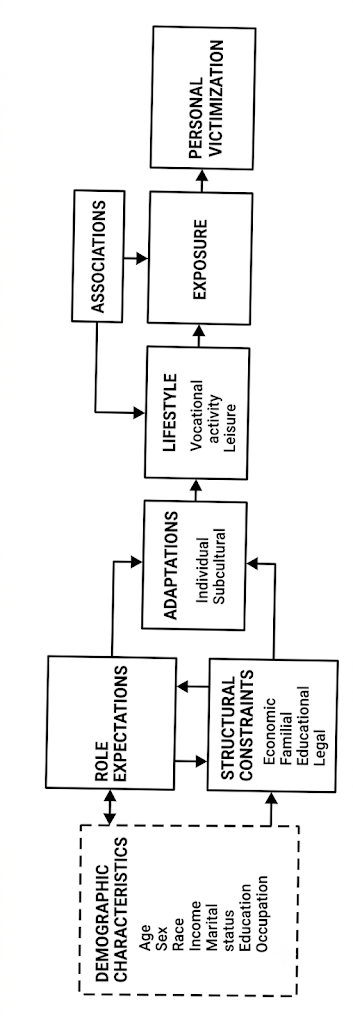
\includegraphics[width=0.5\linewidth]{figures/capitulo3_marco_teorico/3.1_criminologia_ambiental/personal_victimization_model.png}
    \caption{Modelo de la victimización personal.}
    \label{fig:estilo_de_vida_modelo}
    \footnotesize{Nota: Adaptación propia con base en la Figura 11-1 de \cite[p.~243]{hindelang1978}.}
\end{figure}

\subsubsection{Prevención del crimen a través del diseño ambiental}
Acuñada por C. Ray Jeffrey en 1971 en su libro del mismo nombre. En él, argumentó que la modificación de características específicas del diseño urbano reduciría la criminalidad\cite{brantingham1981}. Jeffrey principalmente, establece que\cite{jeffery1971}:

\begin{enumerate}
    \item El crimen puede ser controlado mediante el diseño urbano. Las ciudades son inseguras porque presentan oportunidades para la realización de actos delictivos.
    \item Las ciudades también pueden diseñarse de manera que aumenten el contacto humano, aunque sea de naturaleza íntima. La anomia, la soledad y la alienación no necesariamente caracterizan la vida urbana.
    \item La renovación urbana puede sustituir al sistema de bienestar y se puede poner a las personas a trabajar para construir un entorno que apoye el desarrollo biológico y social de sus habitantes.
\end{enumerate}

\subsubsection{Prevención del crimen situacional}
La prevención del crimen situacional fue propuesta en 1980 por Ronald V. Clarke. Ésta comprende las medidas de reducción de oportunidad que, están dirigidas a formas específicas de crimen; incluyen la gestión, diseño o manipulación del entorno inmediato en una manera tan sistemática y permanente como sea posible; y que hacen al crimen más difícil y riesgoso, o al menos menos beneficioso y excusable para un amplio rango de infractores\cite{clarke1997}.

Algunas de las características más importantes de la definición que nos pueden ayudar a definir de mejor manera este concepto son las siguientes\cite{clarke1997}:

\begin{itemize}
    \item El crimen situacional debe ser diseñada para categorías altamente específicas del crimen. La necesidad de medidas especializadas hacia agresiones particulares no debe ser interpretado como una implicación de que los agresores son especialistas, sino que ciertos crímenes dependen de la construcción de las oportunidades propias de un entorno.
    \item La prevención del crimen situacional no dibuja distinciones entre criminales y las otras personas. Parte de la premisa que todas las personas tienen algo de probabilidad de cometer un crimen dependiendo de las circunstancias.
    \item Cambiar el entorno está diseñado para afectar las evaluaciones hechas por potenciales agresores acerca del costo y los beneficios asociados con cometer un crimen en particular.
    \item Los juicios hechos por potenciales agresores incluyen alguna evaluación del costo moral de agredir. Muchos podemos estar dispuestos a robar pequeños objetos de nuestros empleadores; sin embargo, muy pocos de nosotros estamos dispuestos a robar a una mujer de la tercera edad. Por esto, la moral define en gran medida el alcance del desplazamiento.
    \item Es deliberadamente general para ser aplicable a cualquier tipo de crimen.
\end{itemize}

Asimismo, la prevención situacional del crimen se compone de cuatro componenetes principales. Primero, una base teórica que se apoya principalmente en los enfoques de actividad rutinaria y elección racional; segundo, una metodología estándar basada en el paradigma de la investigación-acción; tercero, un conjunto de técnicas de reducción de oportunidades y finalmente, un cuerpo de prácticas evaluadas que incluye estudios de desplazamiento\cite{clarke1997}.

\subsubsection{Análisis de puntos calientes}
Propuesto por Lawrence Sherman, Patrick Gartin y Michael Buerger en 1989. El artículo busca entender la repetición de la victimización enfocándose en las locaciones individuales como unidad de análisis. En él, los autores establecen que el crimen se concentra de gran manera en solo una serie de ``puntos calientes'' de crimen \cite{sherman1989}. De esta manera, no solo el crimen es más frecuente en algunas ``zonas'' específicas, sino que también el estudio de estas zonas a un nivel micro puede revelar datos mucho más prácticos para la prevención del crimen que el enfoque en áreas más extensas.

El artículo analiza las llamadas de servicio policial en Minneapolis, Minnesota, durante un período de un año, del 15 de diciembre de 1985 al 15 de diciembre de 1986. En él, se examina la distribución de 323,979 llamadas de servicio a lo largo de 115,000 direcciones e intersecciones únicas.

Los hallazgos muestran que pocos ``puntos calientes'' generan la mayoría de las llamadas al servicio policial: poco más del 50\% de las llamadas ocurrieron en solo el 3\% de las direcciones. Esta concentración fue aún más pronunciada en el caso de los delitos predatorios --todos los robos, violaciones y robos de auto ocurrieron en apenas 2.2\%, 1.2\% y 2.7\% de las direcciones, respectivamente. En cuanto a la victimización repetida, el 50\% de las direcciones que generaron una llamada no produjeron más de una; en cambio, el 5\% superior de direcciones experimentó un promedio de 24 llamadas cada una, es decir, una cada dos semanas \cite{sherman1989}.


\subsubsection{Teoría de oportunidades}
La teoría se atribuye a Lawrence E. Cohen, James R. Kluegel y Kenneth C. Land en 1981, en un artículo en el que se buscaba encontrar la relación entre los aspectos de la desigualdad social y el riesgo de la victimización criminal \cite{cohenkluegelland1981}. Como parte de la metodología, examinaron las variables simples del riesgo de victimización, para varios de los delitos más graves y frecuentes, según ingresos, raza y edad. Después, propusieron una teoría de riesgo de victimización depredadora para explicar los resultados obtenidos.

Con esta información, se propone una teoría de oportunidades de la victimización criminal, centrada en el papel mediador que desempeñan cinco factores de riesgo: la exposición, la vigilancia (guardianship), la proximidad a posibles ofensores, el atractivo de los objetivos potenciales, y las propiedades definitorias de los delitos específicos en sí mismos. De este modo, con los resultados obtenidos y como la teoría predijo, se concluyó que en general los grupos socialmente más vulnerables no necesariamente son los más victimizados\cite{cohenkluegelland1981}.

\subsubsection{Síntesis de las bases teóricas}
Es por medio de estas bases teóricas que \textit{la teoría de los patrones delictivos} busca definir que los eventos delictivos no son al azar, pero tampoco son producto de una única teoría. Un enfoque multidisciplinario es la única manera de entender el crimen de manera completa, y justo la teoría de patrones delictivos establece que lo que vemos, es mucho más fácil de entender cuando miramos a través del evento delictivo específico, el sitio, la situación, el trasfondo de la actividad, los patrones probables del delito, los eventos desencadenantes y los factores generales\cite[p.~284]{brantingham1993}.

La teoría propone que todas las investigaciones y todos los argumentos bien razonados apuntan, hacia una etiología compleja como la que se muestra en la figura \ref{fig:patrones_brantingham1993_mejorada}, en la que intervienen múltiples procesos, actividades y motivaciones simultáneamente\cite[p.~273]{brantingham1993}. En esta, los elementos mostrados no son igualmente importantes en cada tipo de crimen o grupo de agresores potenciales. Sin embargo, sin importar que tan poca relevancia tengan, estos nunca desaparecen. Así, los crímenes y la disposición delictiva son entendidos de mejor manera como procesos, matemáticamente como \textbf{funciones} \cite[p.~277]{brantingham1993}.

\begin{figure}
    \centering
    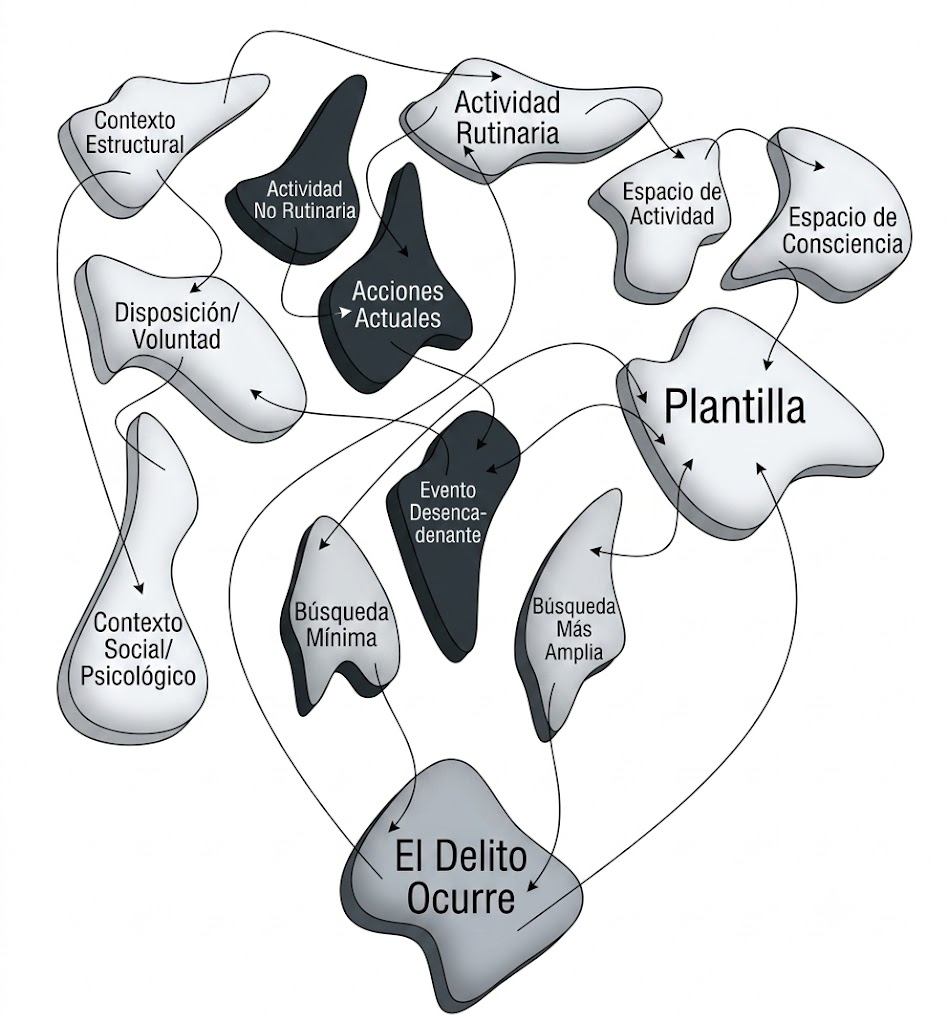
\includegraphics[width=1\linewidth]{figures/capitulo3_marco_teorico/3.1_criminologia_ambiental/teoria_patrones_delictivos_mejorada.png}
    \caption{Procesos, actividades y motivaciones de un crimen}
    \label{fig:patrones_brantingham1993_mejorada}
    \footnotesize{Nota: Adaptación y traducción propia con base en la Figura 11.3 de \cite[p.~284]{brantingham1993}.}
\end{figure}


% =========================================================
% MODELADO DEL TERRENO DE RIESGO (RTM)
% =========================================================
\subsection{Modelado del terreno de riesgo}
El modelado del terreno de riesgo o Risk Terrain Modeling (RTM) es un plan de acción sistemático para estudiar la vulnerabilidad espacial ante el delito\cite{caplan2016}. Identifica los riesgos espaciales que se derivan de las características del paisaje urbano y modela cómo estas se co-localizan para crear entornos únicos para la ocurrencia de delitos específicos\cite{caplan2015}. De esta manera, se busca que factores de riesgo antes tratados como fijos o universales puedan adaptarse a una zona específica con base en su contexto particular y, sobre todo, en los datos disponibles.

El modelo surge como una guía para personas con habilidades básicas en sistemas de información geográfica. Sin embargo, ambos autores desarrollaron a su vez el sistema RTMDx como una implementación técnica que automatiza la mayoría de los pasos analíticos propuestos por el modelo (especialmente los pasos 7 a 9). Así, el proceso actual de RTM y los pasos empleados por el sistema RTMDx son los siguientes\cite[p.~12]{caplan2016}:

\begin{enumerate}
    \item Elegir el evento de resultado
    \item Elegir el área de estudio
    \item Elegir el periodo de tiempo
    \item Identificar los mejores factores de riesgo disponibles
    \item Obtener datos espaciales
    \item Mapear la influencia espacial de los factores
    \item Seleccionar los factores del modelo
    \item Ponderar los factores del modelo
    \item Combinar cuantitativamente los factores del modelo
    \item Comunicar información significativa
\end{enumerate}

% =========================================================
% CONTEXTO GEOGRÁFICO
% =========================================================
\section{Contexto geográfico}
\label{sec:contexto_geografico}

%=========================================================
% CONTEXTO GEOGRÁFICO
%=========================================================

El área de estudio comprende un polígono irregular dentro de la alcaldía Gustavo A. Madero. Para la delimitación espacial del análisis, se seleccionaron específicamente las Zonas Territoriales 6, 7 y 8, establecidas de manera oficial por la demarcación \cite{gam2026}.

\subsection{Delimitación de la zona de estudio}

Como se muestra en la Figura \ref{fig:mapa_zona_estudio}, las Zonas Territoriales 6, 7 y 8 reúnen una gran cantidad de lugares que generan un flujo constante de peatones. Esto se debe a la diversidad de actividades y servicios presentes en la zona, donde se encuentran hospitales, centros comerciales, espacios de entretenimiento e instituciones educativas con una gran cantidad de estudiantes. Además, estas áreas cuentan con distintas opciones de transporte público que facilitan la llegada y el desplazamiento de personas.

La combinación de estos elementos genera una importante concentración de población que se desplaza por la zona en diferentes horarios y con distintos propósitos. Debido a esta variedad de actividades, recorridos y dinámicas de movilidad, se retoman conceptos y teorías de la criminología ambiental para analizar por qué el polígono resulta adecuado para analizar el riesgo al que pueden enfrentarse los peatones.

\begin{figure}[!h]
    \centering
    \includegraphics[width=1\textwidth]{figures/capitulo3_marco_teorico/3.2_contexto_geografico/mapa.png}
    \caption{Delimitación del área de estudio propuesta (Polígono Politécnico-Vallejo). Elaboración propia en QGIS utilizando cartografía base de OpenStreetMap.}
    \label{fig:mapa_zona_estudio}
\end{figure}


\textbf{Infraestructura de transporte} \\
El polígono (especificamente la zona territorial 6 parte de la 7) es atravesado por tres sistemas de transporte público que en conjunto delimitan gran parte de su perímetro. El Sistema de Transporte Colectivo Metro concurre mediante las Líneas 3, 5 y 6: la primera bordea el flanco oriente a través de las estaciones Indios Verdes, Deportivo 18 de Marzo, Potrero y La Raza; la segunda cruza el centro del polígono conectando Politécnico, Instituto del Petróleo, Autobuses del Norte y La Raza; y la tercera enlaza Instituto del Petróleo, Lindavista y Deportivo 18 de Marzo. 

El sistema Metrobús, igual de la zona territorial 6 y parte de la zona 7 concurre mediante dos líneas que enmarcan los bordes poniente y oriente del área: la Línea 3 recorre el corredor Vallejo/Eje 1 Poniente desde Tenayuca hasta La Raza, mientras que la Línea 1 recorre Avenida Insurgentes Norte entre Indios Verdes y La Raza, coincidiendo en ambos casos con estaciones de la red de Metro antes descrita. Por otra parte, en la zona territorial 8 se encuentra una de las unidades más importantes del Instituto Politécnico Nacional: Zacatenco. En esta parte se encuentra una gran parte de transportes concesionados rodeando el area. De igual forma, esta zona tambien abarca casi toda la linea 1 cablebus (Cuautepec-Indios Verdes).

Complementariamente, el Trolebús-linea 8 (Terminal Zacatenco) opera dentro del polígono mediante la Línea 1, que conecta Autobuses del Norte, CCH Vallejo y La Raza, cuyo recorrido es interno a la Unidad Profesional Zacatenco del IPN. Véase la figura \ref{fig:todos_transportes}:\\

\begin{figure}[!h]
    \centering
    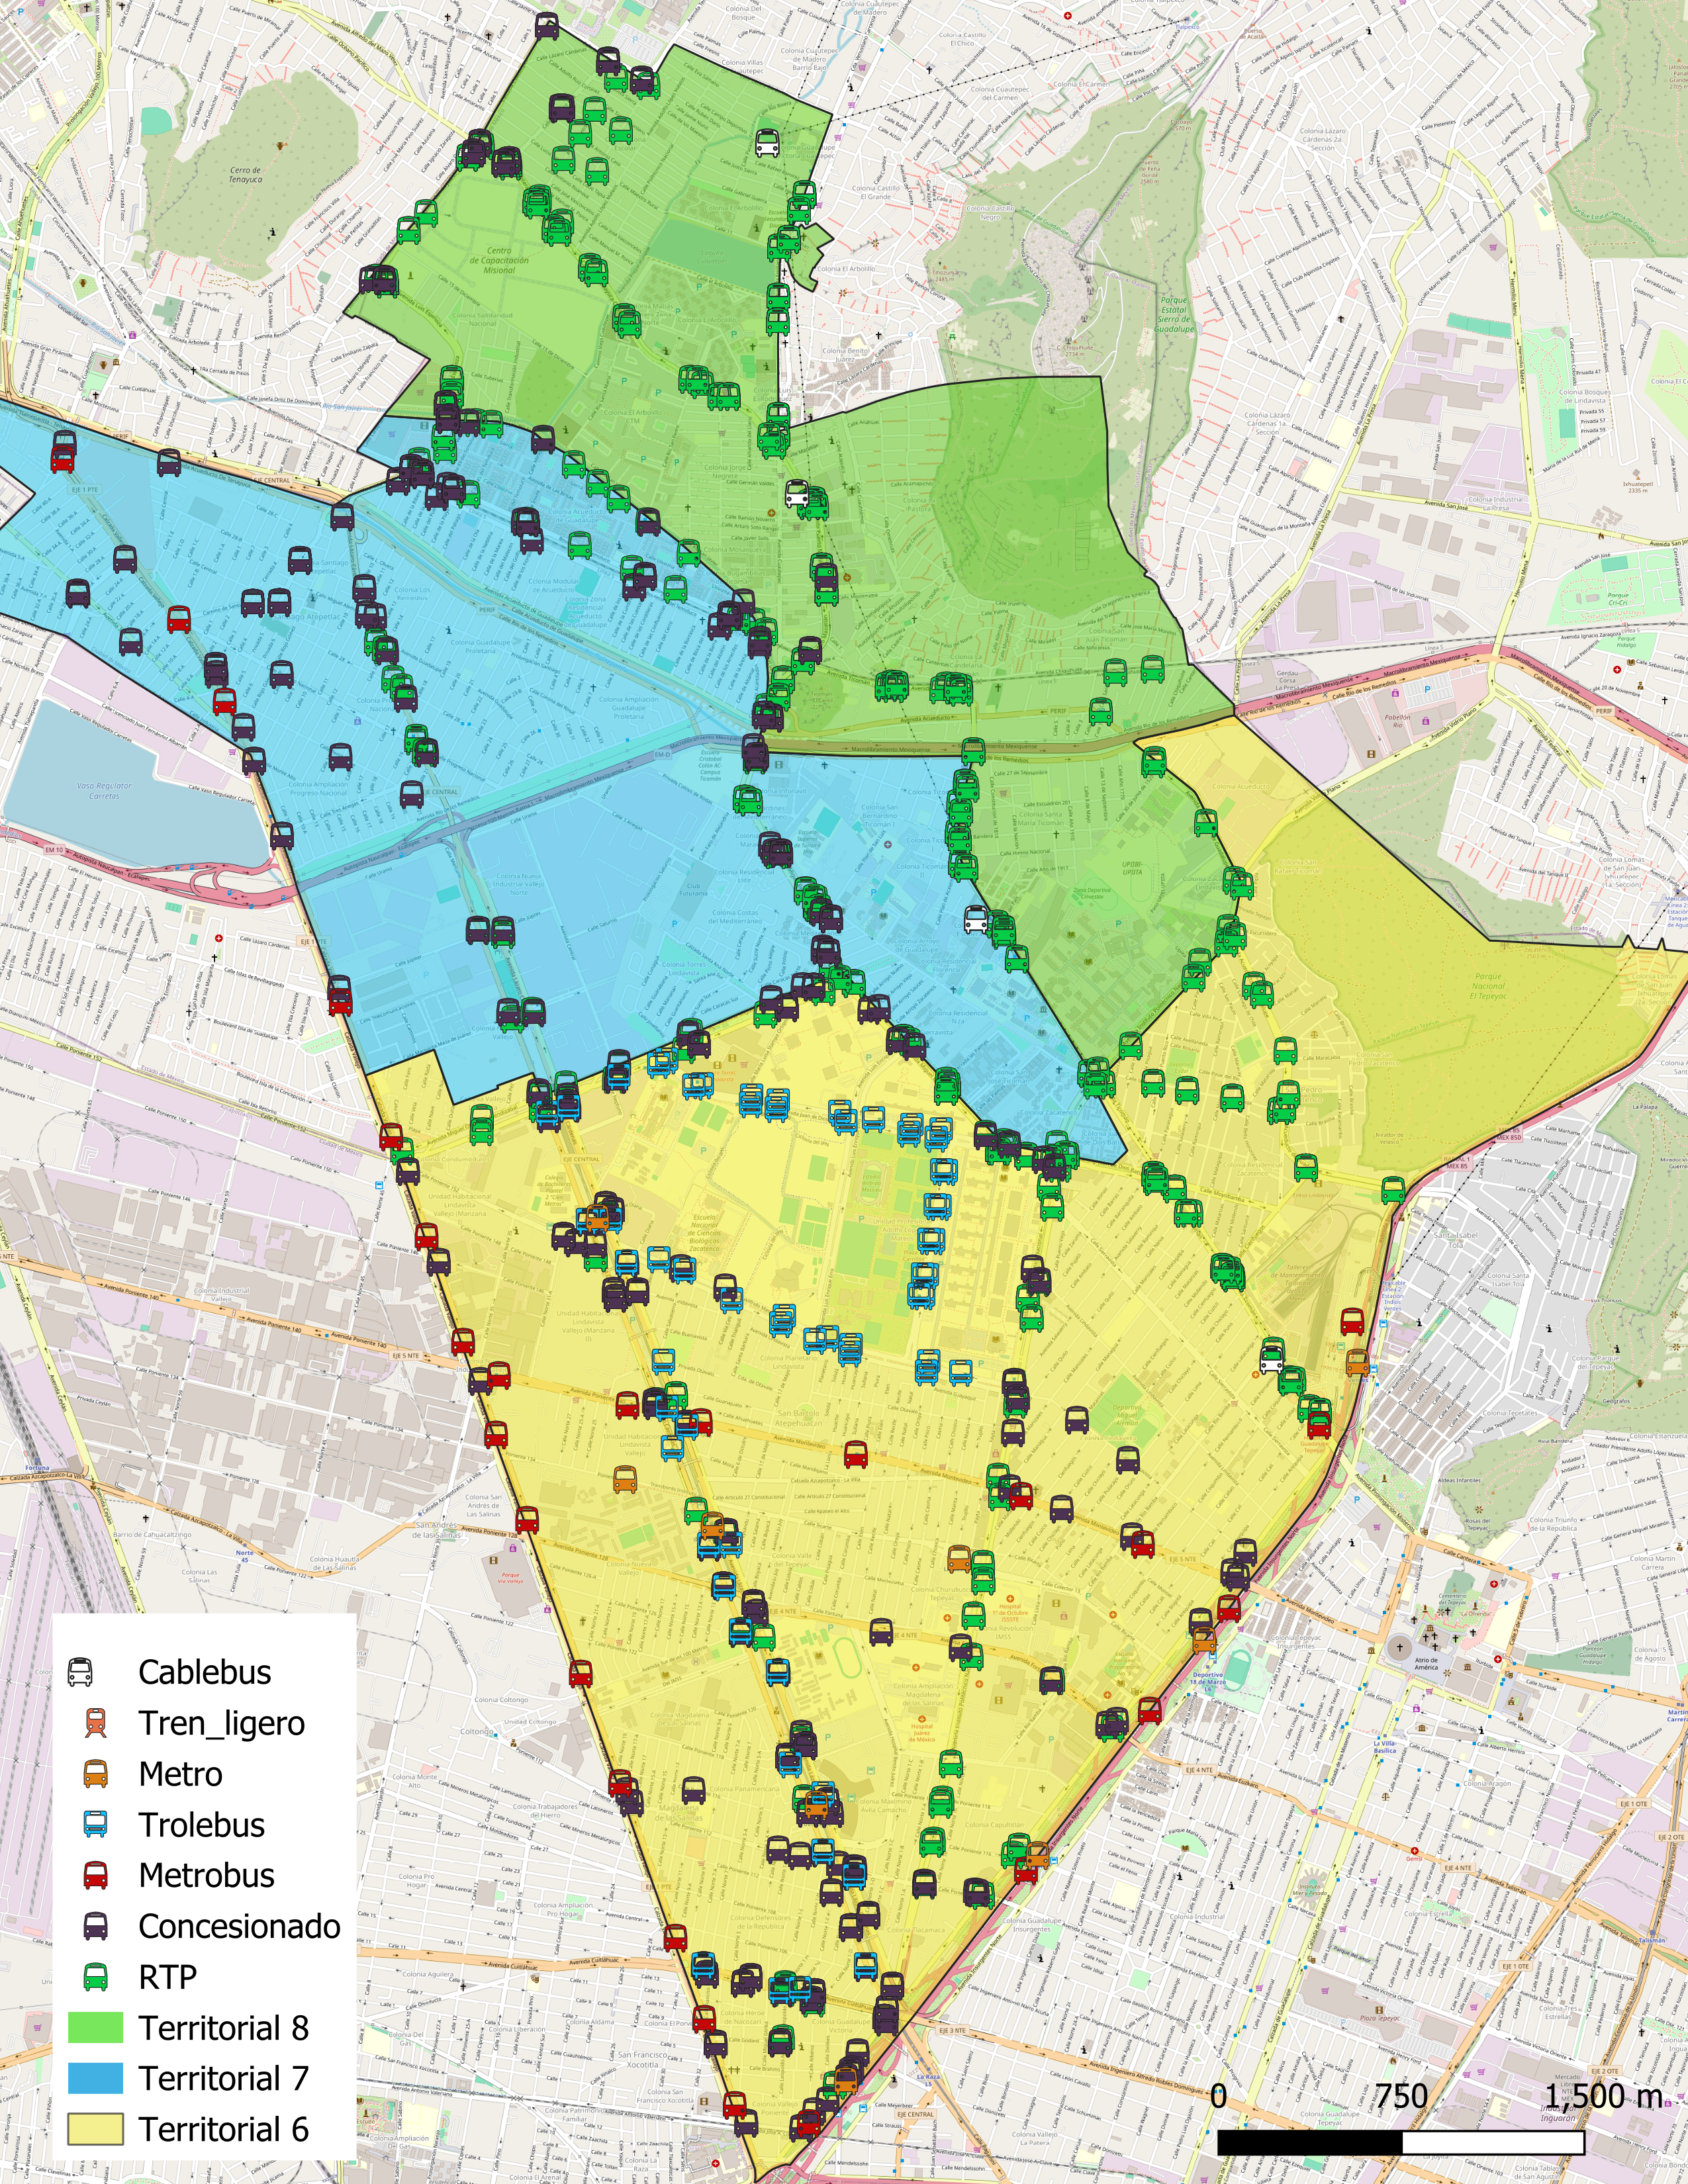
\includegraphics[width=0.8\textwidth]{figures/capitulo3_marco_teorico/3.2_contexto_geografico/transporte.png}
    \caption[Mapa integrado de la red de transporte en las Zonas Territoriales 6, 7 y 8]{Mapa integrado de la red de transporte en las Zonas Territoriales 6, 7 y 8 de la alcaldía Gustavo A. Madero. Elaboración propia mediante el software QGIS.}
    \label{fig:todos_transportes}
\end{figure}

De acuerdo con los registros de la Secretaría de Movilidad \cite{semovi_afluencia2026}, cinco de las rutas que delimitan y cruzan las Zonas Territoriales 6, 7 y 8 figuran dentro del top 18 de mayor demanda en toda la Ciudad de México. Como se detalla en el Cuadro \ref{tab:afluencia_top}, el polígono concentra a la segunda y cuarta ruta más concurridas de toda la red metropolitana (Línea 3 del Metro y Línea 1 del Metrobús). 

\begin{table}[h]
    \centering
    \caption[Afluencia de las líneas de transporte masivo en el polígono de estudio]{Afluencia de las líneas de transporte masivo en el polígono de estudio (Enero - Julio 2026) \cite{semovi_afluencia2026}.}
    
    \vspace{0.2cm}
    \begin{tabular}{|l|c|r|}
        \hline
        \textbf{Sistema y Línea} & \textbf{Lugar a nivel CDMX} & \textbf{Viajes totales} \\ \hline
        STC Metro - Línea 3 & 2$^\circ$ & 96,139,766 \\ \hline
        Metrobús - Línea 1 & 4$^\circ$ & 84,097,297 \\ \hline
        Metrobús - Línea 3 & 14$^\circ$ & 31,681,049 \\ \hline
        STC Metro - Línea 5 & 15$^\circ$ & 31,557,275 \\ \hline
        STC Metro - Línea 6 & 17$^\circ$ & 21,202,436 \\ \hline
    \end{tabular}
    \label{tab:afluencia_top}
\end{table}


Por otra parte, como se resume en el Cuadro \ref{tab:afluencia_transporte}, destaca la estación Indios Verdes con 14.7 millones de viajes en el primer semestre de 2026, cifra que la ubica de forma consistente como la tercera estación de mayor afluencia de toda la red \cite{stcmetro2026}. En contraste, Instituto del Petróleo registra el volumen más bajo del polígono, con 1.3 millones de viajes entre sus dos lineas. \cite{stcmetro2026}.


Entre enero y julio de 2026, la Línea 1 del metrobús registró 84,097,297 viajes totales, siendo la línea de mayor demanda de todo el sistema Metrobús (31\% del total de la red), mientras que la Línea 3 registró 31,681,049 viajes en el mismo periodo (11\% del total) \cite{semovi2026mb}.

En el mismo periodo, la Línea 1 del trolebús acumuló 11,841,056 viajes, mientras que la Línea 8 registró apenas 905,878 \cite{semovi2026tb}, cifra considerablemente menor que se explica por la naturaleza interna y de corta distancia de su recorrido dentro del campus.

\begin{table}[h]
\centering
\caption{Afluencia de estaciones y líneas de transporte masivo dentro del área de estudio.}
\label{tab:afluencia_transporte}
\begin{tabular}{llr}
\toprule
\textbf{Estación / Línea} & \textbf{Sistema} & \textbf{Viajes (2026)} \\
\midrule
Indios Verdes & Metro L3 & 14,743,513 \\
La Raza & Metro L3 + L5 & 6,222,363 \\
Deportivo 18 de Marzo & Metro L3 + L6 & 4,531,655 \\
Politécnico & Metro L5 & 4,288,865 \\
Autobuses del Norte & Metro L5 & 3,124,764 \\
Lindavista & Metro L6 & 2,498,111 \\
Potrero & Metro L3 & 2,180,907 \\
Vallejo & Metro L6 & 1,138,453 \\
Instituto del Petróleo & Metro L5 + L6 & 1,335,956 \\
\midrule
Línea 1 & Metrobús & 84,097,297 \\
Línea 3 & Metrobús & 31,681,049 \\
\midrule
Línea 1 & Trolebús & 11,841,056 \\
Línea 8 (Circuito Politécnico) & Trolebús & 905,878 \\
\bottomrule
\end{tabular}
\end{table}

Tener los datos aproximados de afluencia de personas en las estaciones de transporte público es importante para esta investigación porque estos espacios funcionan como nodos de actividad que concentran grandes volúmenes de desplazamientos diarios. De acuerdo con la teoría de los patrones delictivos de Brantingham y Brantingham 
\cite[p.~259-294]{brantingham1993}, la búsqueda de objetivos por parte de un delincuente y/o agresos no es aleatoria, sino que ocurre a lo largo de las rutas de tránsito habitual y en los nodos donde convergen diversas personas. En el contexto local, la evidencia confirma esta premisa; Fuentes y Sánchez \cite{fuentes2017} demostraron que las estaciones de transbordo tienen un efecto positivo estadísticamente significativo en los índices de criminalidad, estimando que un incremento del 10\% en esta variable se asocia con un aumento del 5.4\% en los robos a transeúntes. Es por esta razón por la que cuantificar la afluencia permite dimensionar e identificar las zonas de mayor exposición para los usuarios y mapear con precisión las áreas donde se requiere priorizar la seguridad.
 \\

\textbf{Zonas Industriales, Habitacionales y Escolares} \\


Como se estableció en la delimitación de la zona de estudio, el área analizada está conformada por las Zonas Territoriales 6, 7 y 8 de la alcaldía Gustavo A. Madero. Dentro de este espacio se identifican áreas industriales, habitacionales y escolares con diferentes características y funciones dentro del entorno urbano. En particular, el área de estudio no contiene extensiones de uso industrial, salvo los sectores correspondientes a Nueva Industrial Vallejo y Nueva Vallejo (Véase figura \ref{fig:uso_suelo}), mientras que sus fronteras poniente y sur colindan con corredores industriales de mayor escala. Por otra parte, el uso de suelo habitacional ocupa una parte importante del área analizada y se distribuye a lo largo de las tres Zonas Territoriales, como se observa en el mapa de uso de suelo (Figura \ref{fig:uso_suelo}). Asimismo, dentro del área de estudio se localizan diversos planteles educativos de distintos niveles, cuya distribución se muestra, de igual forma, en la Figura \ref{fig:escuelas}.

\begin{figure}[!h]
    \centering
    \includegraphics[width=0.8\textwidth]{figures/capitulo3_marco_teorico/3.2_contexto_geografico/uso_suelo.png}
    \caption[Mapa de uso de suelo: zonas habitacionales e industriales en el área de estudio]{Mapa de uso de suelo en las Zonas Territoriales 6, 7 y 8 de la alcaldía Gustavo A. Madero, destacando las áreas habitacionales y las zonas industriales (puntos morados). Elaboración propia mediante el software QGIS.}
    \label{fig:uso_suelo}
\end{figure} 

\textbf{Zonas Industriales} \\
El entorno de la zona de estudio presenta una combinación de áreas industriales que se encuentran dentro de la alcaldía Gustavo A. Madero y otros sectores industriales ubicados fuera de esta demarcación, pero que colindan directamente con el polígono de estudio. Esta distinción resulta relevante debido a que los sectores ubicados en los límites de la zona de estudio concentran puntos de acceso y conexión con el transporte público, por lo que pueden formar parte de los recorridos peatonales de las personas que se desplazan hacia o desde las áreas industriales.

Dentro de la alcaldía Gustavo A. Madero, por el flanco poniente, se encuentran Nueva Industrial Vallejo y Nueva Vallejo. La primera presenta una superficie aproximada de 1.17 km² (12,627,764.43 pies²) y una distancia total aproximada de 4.93 km (3.06 mi) \cite{googlemaps2026}. De acuerdo con los registros de la Fiscalía General de Justicia de la Ciudad de México, en este sector se documentaron 7 robos a transeúnte, 4 casos de violación, uno de ellos correspondiente a 2024, y un homicidio doloso durante 2025 \cite{FGJ2025}. Para el periodo de enero a julio de 2026 se registraron nuevamente 7 robos a transeúnte, un caso de violación y un robo a cuentahabiente \cite{FGJ2026}.

Por su parte, Nueva Vallejo cuenta con una superficie aproximada de 403,004.52 m² (4,337,904.52 pies²) y una distancia total aproximada de 3.82 km (2.37 mi) \cite{googlemaps2026}. En este sector se documentó, durante 2024, una carpeta de investigación por robo a transeúnte y una por violación \cite{FGJ2025}. Para 2025 se registraron 7 robos a transeúnte y un caso de violación \cite{FGJ2025}, mientras que durante enero-julio de 2026 se documentaron 4 carpetas por robo a transeúnte, todas tipificadas con violencia, y una denuncia adicional por violación \cite{FGJ2026}.

Fuera de la alcaldía Gustavo A. Madero, pero en contacto directo con el límite del área de estudio, se encuentran otros sectores que forman parte del entorno inmediato. En el vértice sur, el polígono colinda con Santa María Insurgentes y Atlampa, ambas ubicadas en la alcaldía Cuauhtémoc. En conjunto, estos sectores presentan una superficie aproximada de 1.59 km² (17,081,745.16 pies²) y una distancia total de 6.07 km (3.77 mi) \cite{googlemaps2026}. De acuerdo con los registros de la Fiscalía General de Justicia, durante 2025 se documentaron en este sector 13 carpetas de investigación por robo a transeúnte en vía pública, 4 casos de homicidio doloso y 2 denuncias por violación \cite{FGJ2025}. Para el periodo de enero a julio de 2026 se registraron 4 incidentes adicionales por robo a transeúnte y un caso de violación \cite{FGJ2026}.

De manera complementaria, en el entorno inmediato también se encuentra la Zona Industrial Vallejo, ubicada en la alcaldía Azcapotzalco, en colindancia con Gustavo A. Madero. Este polígono presenta una superficie aproximada de 3.76 km² (1.45 mi²) y una distancia total aproximada de 11.58 km (7.19 mi) \cite{googlemaps2026}. En 2024 se registró en este sector una carpeta por robo a transeúnte y una por violación, mientras que durante 2025 se documentaron 2 incidentes de robo a transeúnte \cite{FGJ2025}. Para enero-julio de 2026 se registraron 8 carpetas por robo a transeúnte en la vía pública, todas tipificadas con violencia, y un caso de violación \cite{FGJ2026}.

La incorporación de estos sectores externos no implica que formen parte del área de estudio, sino que permite caracterizar las condiciones existentes en sus límites y en los puntos donde se establece la conexión con el entorno urbano circundante. Esta relación resulta especialmente relevante debido a que las zonas industriales presentan una disponibilidad limitada de transporte público en su interior, por lo que los principales puntos de acceso y conexión se concentran en sus bordes \cite{googlemaps2026}. En consecuencia, las personas que se desplazan hacia estos sectores pueden realizar recorridos peatonales desde dichos puntos hasta sus lugares de trabajo, haciendo que las condiciones de las vialidades y espacios públicos ubicados en sus límites sean relevantes para el análisis.

De acuerdo con los principios de la Prevención del Delito Mediante el Diseño Ambiental (CPTED), propuesta por C. Ray Jeffrey en 1971 \cite{jeffery1971}, esta situación puede representar una mayor vulnerabilidad para los peatones. Las zonas industriales suelen presentar una configuración urbana poco diversa, en la que predominan grandes espacios destinados a una sola actividad. Es común encontrar muros extensos, fachadas con pocas ventanas y poca presencia de comercios, personas o viviendas en las calles.

Estas condiciones pueden reducir la vigilancia natural, es decir, la posibilidad de que otras personas observen lo que ocurre en el espacio público. El problema puede ser mayor fuera de los horarios de entrada y salida de los trabajadores, cuando disminuye considerablemente la cantidad de personas en las calles. Desde la perspectiva de Jeffrey, las características del entorno pueden influir en las oportunidades para cometer delitos, ya que el aislamiento y la poca interacción entre las personas facilitan que ciertas zonas sean menos visibles y transitadas.

\textbf{Zonas Habitacionales} \

El uso de suelo habitacional ocupa una parte importante de la zona de estudio y se distribuye a lo largo de las tres Zonas Territoriales, como se observa en la Figura \ref{fig:uso_suelo}. Estas áreas corresponden principalmente a espacios destinados a la residencia de la población y permiten identificar zonas en las que se concentra parte de la actividad cotidiana asociada con el ámbito doméstico.

La distribución de las zonas habitacionales resulta relevante para el análisis de movilidad debido a que pueden constituir puntos de origen de desplazamientos hacia otros espacios donde se desarrollan actividades cotidianas, como centros educativos, lugares de trabajo, comercios y otros servicios. Sin embargo, su ubicación no permite determinar por sí misma los recorridos realizados por la población, por lo que su función dentro del análisis se considera como parte de la estructura espacial a partir de la cual posteriormente se representarán posibles desplazamientos mediante el grafo de movilidad.


\textbf{Zonas Escolares} \\


De manera complementaria, el área de estudio cuenta con diversos planteles educativos distribuidos entre las tres Zonas Territoriales. Como se observa en la Figura \ref{fig:escuelas}, se identifican instituciones de distintos niveles educativos. Entre estas instituciones destaca la presencia de instalaciones del Instituto Politécnico Nacional.

\begin{figure}[!h]
    \centering
    \includegraphics[width=0.8\textwidth]{figures/capitulo3_marco_teorico/3.2_contexto_geografico/escuelas.png}
    \caption[Escuelas de nivel superior, medio superior, secundarias y básicas]{Mapa de escuelas de nivel superior, medio superior, secundarias y básicas en las Zonas Territoriales 6, 7 y 8 de la alcaldía Gustavo A. Madero. Elaboración propia mediante el software QGIS.}
    \label{fig:escuelas}
\end{figure}

La presencia de instituciones educativas permite identificar espacios en los que se desarrollan actividades recurrentes de la población, particularmente aquellas relacionadas con la formación académica. Su distribución dentro del área de estudio resulta relevante para el análisis de movilidad debido a que estos espacios pueden constituir destinos frecuentes para estudiantes, docentes y personal administrativo.

La importancia de las instituciones educativas dentro del área de estudio puede observarse particularmente en el caso del Instituto Politécnico Nacional. De acuerdo con Data México, en 2022 el IPN registró 128,869 estudiantes matriculados en la Ciudad de México, mientras que 56,450 correspondieron a Gustavo A. Madero \cite{datamexico_ipn}. Estos datos permiten dimensionar la presencia de la institución en la demarcación. Además, el propio IPN señala que en la Unidad Profesional ``Adolfo López Mateos'' convergen diariamente más de 30 mil alumnos y 5 mil docentes e investigadores en un área aproximada de 2.5 kilómetros de largo por 2.5 kilómetros de ancho\cite{ipn2022}.

\textbf{Las actividades rutinarias como punto de partida} \

La distribución conjunta de las zonas habitacionales, escolares e industriales puede analizarse a partir de la teoría de las actividades rutinarias propuesta por Cohen y Felson. Los autores definen las actividades rutinarias como aquellas actividades recurrentes y habituales que forman parte de la vida cotidiana y permiten cubrir distintas necesidades de la población, como el trabajo, la obtención de alimentos, el ocio y la interacción social \cite{cohenfelson1979}. Estas actividades se desarrollan en diferentes lugares, por lo que pueden generar desplazamientos entre los espacios donde las personas residen y aquellos donde realizan sus actividades cotidianas.

Desde esta perspectiva, las zonas habitacionales pueden representar posibles puntos de origen, mientras que las instituciones educativas y las áreas industriales pueden corresponder a espacios vinculados con actividades que generan desplazamientos recurrentes. En particular, los sectores industriales constituyen espacios relacionados con actividades laborales, mientras que las instituciones educativas concentran actividades académicas que se desarrollan de manera periódica. La ubicación de estos elementos permite, por tanto, identificar relaciones espaciales entre lugares de residencia y algunos de los posibles destinos asociados con las actividades cotidianas, sin asumir de antemano los recorridos que realizan las personas.

Estos datos no permiten determinar por sí mismos los recorridos realizados por estudiantes, docentes, trabajadores o residentes, pero sí muestran la existencia de espacios con diferentes concentraciones y tipos de actividad cotidiana. De acuerdo con Cohen y Felson, la distribución de estas actividades fuera del hogar puede generar la convergencia de personas en determinados lugares y momentos, modificando las oportunidades para la ocurrencia de delitos \cite{cohenfelson1979}. En este sentido, la oportunidad constituye un elemento relevante para analizar la relación entre las actividades cotidianas, la movilidad y el delito \cite{canopanos2018}.

Por lo tanto, las zonas habitacionales, escolares e industriales no se consideran por sí mismas como espacios de mayor o menor riesgo. Su inclusión en el análisis responde a su relación con las actividades cotidianas de la población y a su posible función como puntos de origen o destino dentro de los desplazamientos que serán representados mediante el grafo de movilidad.


\subsubsection{Síntesis del contexto geográfico}

El análisis realizado permite identificar que las Zonas Territoriales 6, 7 y 8 presentan una combinación de espacios asociados con distintas actividades y desplazamientos cotidianos. En el área de estudio se encuentran zonas habitacionales, instituciones educativas, zonas industriales y una red de transporte público, cuya distribución permite caracterizar parte de las condiciones espaciales en las que se desarrollan las actividades de la población.

Esta configuración puede interpretarse a partir de la teoría de las actividades rutinarias, ya que las actividades cotidianas se desarrollan en distintos lugares y pueden generar desplazamientos entre ellos \cite{cohenfelson1979}. Desde esta perspectiva, la distribución de los espacios habitacionales, educativos e industriales permite identificar posibles relaciones entre lugares de residencia y destinos asociados con actividades cotidianas, mientras que la red de transporte constituye parte de la infraestructura mediante la cual se realizan estos desplazamientos.

A su vez, las características físicas de determinados espacios, particularmente de las zonas industriales, permiten incorporar elementos de la Prevención del Delito Mediante el Diseño Ambiental. Aspectos como el aislamiento, la configuración de los espacios y las condiciones de vigilancia natural pueden ser considerados dentro del análisis del entorno construido. Estos elementos se complementan con los registros oficiales de delitos y la información disponible sobre percepción de inseguridad, considerando que las estadísticas delictivas no representan la totalidad de los hechos ocurridos debido a la existencia de una cifra negra.

En conjunto, esta información permite caracterizar el contexto geográfico de la zona de estudio y establecer los elementos que serán considerados en el análisis posterior. A partir de la distribución de los distintos tipos de espacios y de la red vial, se construirá el grafo de movilidad, en el que las vialidades y sus conexiones constituirán la base para representar los desplazamientos peatonales. Posteriormente, los factores identificados en el contexto geográfico y los registros de delito serán incorporados al análisis de los tramos de la red para determinar los componentes que intervienen en el cálculo del costo de desplazamiento y, finalmente, en la generación de rutas peatonales.


% =========================================================
% TEORÍA DE GRAFOS
% =========================================================
\newpage 
\section{Teoría de grafos}
% ======================================
% TEORIA DE GRAFOS 
% ======================================
La teoría de grafos es una rama de las matemáticas y las ciencias de la computación orientada al estudio de las propiedades de los grafos, los cuales son abstracciones matemáticas utilizadas para modelar relaciones e interconexiones entre distintos objetos.

En definición un grafo en computación es una estructura de datos no lineal conformada por un conjunto de objetos llamados nodos los cuales están conectados por medio de aristas (o arcos). Utilizar grafos facilita la representación y el análisis de sistemas complejos dentro de los cuales se encuentran por ejemplo, las redes de transporte. 

\subsection{El problema del camino más corto}

Dentro de la teoría de grafos el Problema del Camino Más Corto o SPP por sus siglas en ingles (Shortest Path Problem), consiste en encontrar una ruta con el menor costo, distancia o tiempo entre dos vértices o nodos dentro de un grafo ponderado. El concepto de SPP es muy conocido dentro del panorama computacional ya que es comúnmente utilizado en diferentes aplicaciones o software de la vida cotidiana teniendo como mayor ejemplo al famoso Google Maps, siendo este el caso más conocido de la aplicación de la teoría de grafos en problemas SPP aplicando algoritmos de búsqueda para encontrar el camino más corto desde un nodo origen hacia un nodo destino por medio de una serie de aristas interconectadas entre múltiples nodos las cuales forman finalmente el grafo, dichos nodos representan las locaciones conocidas en el mundo real, las aristas los posibles caminos como calles o vialidades a disposición que interconectan los nodos y el grafo siendo la representación completa del mapa, zona, área o región mediante nodos y aristas. 

Dentro del ámbito de los grafos existen diversos tipos, y cada uno se adapta a diferentes necesidades o entornos por lo que es de vital importancia elegir de la mejor manera el tipo de grafo adecuado para el problema de esquematizar la zona de la alcaldía Gustavo A. Madero. Con el objetivo de solucionar la problemática planteada dentro del trabajo terminal, se evalúan los siguientes tipos principales de grafos:

\newpage

\subsection{Tipos de Grafos}

\subsubsection{Grafos dirigidos y no dirigidos} 
Dentro de un grafo dirigido las aristas tienen una dirección la cual indica el flujo de desplazamiento entre nodos, es decir, indican de que forma dentro del grafo podemos movernos entre nodos siguiendo la dirección de las aristas. Es común ver este tipo de grafo para flujo de trabajo o diagramas de procesos, donde el orden y la secuencia de los pasos importa. 

Con respecto a los grafos dirigidos, estos son su contraparte, por lo que las aristas no tienen dirección. Esto significa que la relación entre los nodos es bidireccional dando la posibilidad de poder transitar entre nodos en cualquier dirección por medio de las aristas. Este tipo de grafos suele utilizarse para representar relaciones reciprocas donde no importa la dirección o la secuencia entre nodos. 

\begin{figure}[h]
    \centering
    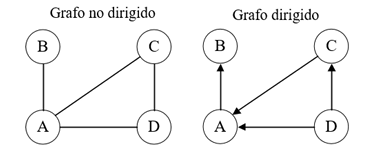
\includegraphics[width=0.6\textwidth]{figures/seccion3_5/grafo_dirigidoyno.png}
    \caption{Representación topológica de los grafos dirigidos y no dirigidos}
    \label{fig:grafo_dirigino-no}
\end{figure}

\subsubsection{Grafos ponderados y no ponderados} 
Existen grafos que incluyen pesos en sus aristas o valores numéricos los cuales representan el costo de la relación entre nodos. Usualmente este tipo de nodos son utilizados para representar relaciones donde el valor de las conexiones es importante para el problema, por ejemplo, en el caso de redes viales las aristas pueden integrar valores que representen la distancia entre nodos para después poder aplicar operaciones sobre dichos valores. 

En caso contrario el grafo no ponderado carece de información o etiquetas asociadas a las aristas. 

\begin{figure}[h]
    \centering
    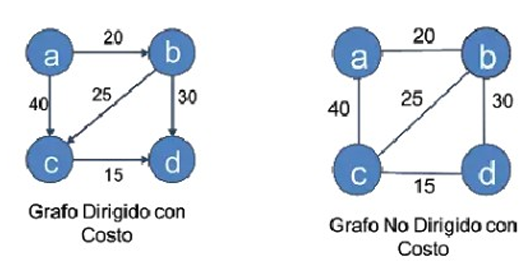
\includegraphics[width=0.8\textwidth, height=0.2\textheight, keepaspectratio]{figures/seccion3_5/grafo_ponderado y no ponderado.png}
    \caption{Representación topológica de los grafos ponderados y no ponderados}
    \label{fig:grafon_pond_no}
\end{figure}

\subsubsection{Grafos cíclico y acíclicos}
Los grafos cíclicos contienen al menos un ciclo, un camino que comienza y termina en el mismo nodo. En los grafos cíclicos los vértices son componentes y las aristas representan conexiones lo que nos permite formar ciclos de corriente o un flujo de transición cíclico, es decir, que en alguno punto retorna al nodo de inicio donde se encontró por primera vez un ciclo. 

Al contrario los grafos acíclicos no tienen ningún ciclo. En la mayoría de los casos este tipo de grafos se utiliza para representar puramente relaciones y no secuencias. 

\begin{figure}[h]
    \centering
    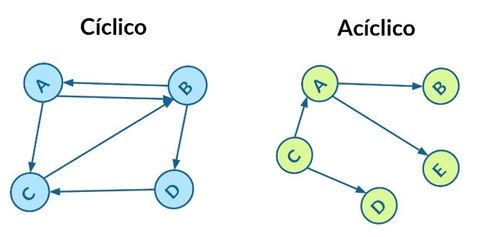
\includegraphics[width=0.8\textwidth, height=0.15\textheight, keepaspectratio]{figures/seccion3_5/grafio_ciclico_y_aciclico.png}
    \caption{Representación topológica de los grafos cíclicos y acíclicos}
    \label{fig:grafon_ciclico_no}
\end{figure}

\subsubsection{Grafos simples y multigrafos}
Un grafo simple se define como aquella estructura matemática donde un conjunto no vacío de vértices se interconecta a través de aristas únicas, restringiendo la existencia de trayectos paralelos entre un mismo par de nodos. 

Por su parte, un multigrafo representa una composición estructural de mayor complejidad, en la cual los nodos pueden interconectarse mediante múltiples aristas paralelas o alternativas. Esta característica permite modelar diferentes rutas o variables que coexisten entre los mismos puntos del entorno.

\begin{figure}[h]
    \centering
    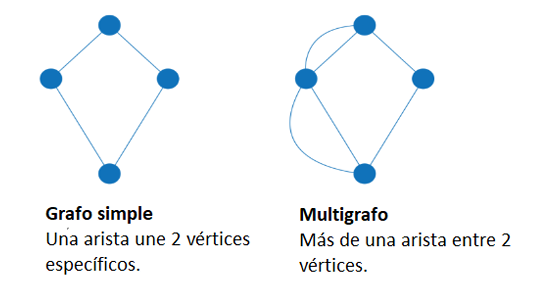
\includegraphics[width=0.8\textwidth, height=0.2\textheight, keepaspectratio]{figures/seccion3_5/grafo_simple .png}
    \caption{Representación topológica de los grafos simples y multigrafos}
    \label{fig:grafon_simp_no}
\end{figure}

\newpage

\subsubsection{Grafos conexos y no conexos}
En el análisis de redes topológicas, un grafo conexo se define como aquella estructura donde existe, al menos, un camino transitable entre cualquier par de vértices que lo componen. 

Por el contrario, un grafo no conexo presenta una fragmentación en su arquitectura, generando subgrafos o nodos aislados que carecen de enlaces con el entramado principal. 

\begin{figure}[h]
    \centering
    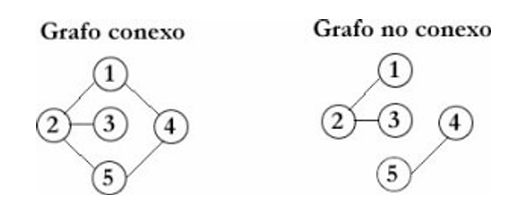
\includegraphics[width=0.8\textwidth, height=0.15\textheight, keepaspectratio]{figures/seccion3_5/grafo_conexo_y_no.png}
    \caption{Representación topológica de los grafos simples y multigrafos}
    \label{fig:grafon_con_no}
\end{figure}

\subsubsection{Elección y Justificación del tipo de grafo adecuado a la problemática presente}

Como se pudo apreciar hay bastantes tipos de grafos a tomar en cuenta sin embargo podemos decir con seguridad que lo más adecuado al problema es un grafo ponderado no dirigido con características del grafo simple, conexo y el cíclico. Al estar trabajando dentro de una demarcación territorial clasificada como localidad donde hay desplazamiento de vehículos e individuos constantemente, lo ideal es que los transcursos como calles o avenidas (aristas en el caso del grafo) estén sujetas a cierto peso debido a que esta información resulta útil para el calculo de rutas en la aplicación, en cuanto a la dirección realmente no es importante pues en la mayoría de transcursos el desplazamiento o traslado es bidireccional.

Cabe mencionar que en su mayoría la extensión territorial se rige por principios de un grafo simple ya que existe por lo menos un camino que conecte las múltiples ubicaciones o nodos del grafo. 

En cuanto al hecho de mantenerlo conexo es en relación a que en la localidad en la que el proyecto se esta desarrollando no se tienen zonas apartadas sin posible acceso, al contrario, todas las locaciones tiene un camino para trasladarse de un punto de origen a un punto de destino lo que evita caer en un grafo inconexo, ademas de que ser prácticamente imposible mapear un camino o ruta hacia nodos inaccesibles en caso de trabajar con zonas que se representen mediante grafos no conexos. También se integrarían elementos de un grafo cíclico ya que podemos retornar por múltiples caminos al nodo o locación de origen por ejemplo podemos volver a un punto de partida dando la vuelta a una manzana. 

\newpage

\subsection{Análisis de algoritmos de optimización en grafos}

\textbf{Algoritmos para problemas del camino más corto} \\
\label{AgSPP}

Existen una gran variedad de algoritmos que se encargan de resolver el \textbf{"Problema del camino más corto"} de múltiples formas, sin embargo, para este caso en particular no solo buscamos encontrar la ruta con menor costo de un punto a otro, también se integrara la inseguridad peatonal como variable compuesta de factores ambientales, sociales, estructurales y geográficos para obtener la generación de una ruta de transporte que tenga en cuenta los posibles factores de riesgo que pueden provocar un daño a la integridad de los peatones con la finalidad de balancear entre velocidad y seguridad para los usuarios. 

Es debido a la cantidad variada de algoritmos para problemas SPP (Shortest Path Problem) que debemos analizar los más adecuados al proyecto en busca de la mejor alternativa por lo que a continuación veremos en que consisten algunos de los algoritmos mas utilizados en la actualidad y con mayor eficiencia respecto a la optimización de grafos sin dejar de tomar en cuenta que tan benéficos y flexibles son para el proyecto considerando que deben trabajar con una variable extra, la inseguridad de los transcursos.

\subsubsection{Principales Algoritmos utilizados en problemas SPP}

En el ámbito de la informática y la computación existen múltiples algoritmos enfocados en la búsqueda de las rutas más optimas dentro de grafos ponderados sin embargo hay algoritmos que destacan sobre otros debido a su gran eficiencia y optimización provocando que en la actualidad sean un estándar al momento de resolver problemas de esta índole ya sea como base de un programa o como apoyo para desarrollar una mejora a partir de este grupo selecto de algoritmos, dentro los cuales se encuentran los siguientes: 

\subsubsection{Algoritmos de Origen Único (Single-Source)}
Dentro de esta sección se encuentran los algoritmos enfocados en buscar la ruta óptima desde un vértice inicial específico hacía uno o todos los demás nodos en la red. 

\begin{itemize}
    \item \textbf{Algoritmo de Dijkstra:} Garantiza encontrar la solución óptima global iterando siempre sobre el menor costo acumulado. Algunos algoritmos iteran sobre un grafo en busca de la solución más optima pero en veces no toman en cuenta todas las alternativas disponibles dentro del grafo y sus múltiples conexiones lo que provoca que al encontrar una solución al final de la iteración, esta misma sea un optimo local, es decir, una solución que es factible para esa ejecución en particular la cual tiene probabilidad de no ser la mejor de todas al no tomar en cuenta todas las alternativas. Dijkstra soluciona el problema del optimo local mediante el calculo de costo acumulado teniendo como único problema que el algoritmo no funciona para ponderaciones negativas lo que lo vuelve el estándar para redes viales urbanas donde las distancias físicas impiden la existencia de pesos negativos. 

    Dijkstra toma un nodo inicial (por ejemplo la dirección de un negocio o casa) y comienza a explorar todas las rutas posibles hacia el nodo de destino mientras lleva el calculo de la distancia acumulada en las diferentes posibilidades de trayectos los cuales se utilizaron para llegar al destino. Inicialmente parte del nodo de origen, "visita" primero al nodo más cercano y con menor coste para posteriormente trasladarse a dicho nodo y seguir repitiendo el proceso seleccionando siempre el camino de menor distancia acumulada conforme van aumentando los desplazamientos entre nodos. Es justo de esta forma como el algoritmo cada que llega a un nuevo "cruce", revisa, reconsidera y actualiza la distancia más corta registrada hasta el punto en el que se encuentra actualmente. En caso de encontrar una ruta más corta a una ubicación que ya había sido visitada por otro camino, el algoritmo reajusta el cálculo para reestructurar sus decisiones junto con la ruta que actualmente esta en ejecución hasta que finalmente consigue llegar al destino por medio del mejor camino posible \cite{dijkstra_udit}. 

    Dijkstra sigue siendo uno de los algoritmos de búsqueda para el camino más corto más importantes del panorama informático en general por lo que es una alternativa altamente útil al momento de aplicarlo sobre la propuesta de software "Prototipo de aplicación móvil para la generación de rutas peatonales seguras dentro de la alcaldía Gustavo A. Madero". 
    
    \item \textbf{A-Star (A*):} El algoritmo de A* se base en los principios fundamentales de Dijkstra que lo vuelven tan solido y añade una capa extra de inteligencia integrando la heurística o "intuición" como parte fundamental de la búsqueda \cite{dijkstra_udit}. 

    Antes de profundizar en el funcionamiento del algoritmo A*, primero debemos entender el concepto que se introduce con el uso de este algoritmo, la \textbf{heurística}. En el ámbito de la inteligencia artificial y la búsqueda en grafos, una heurística es un atajo mental, o mejor dicho, un conjunto de diferentes métodos, técnicas o estrategias que permiten solucionar un problema, tomar decisiones, emitir juicios o realizar descubrimientos de forma rápida y práctica.

    Las heurística nos permiten reducir drásticamente el tiempo y la energía invertida en la resolución de problemáticas sin embargo muchas veces resultan en conclusiones erróneas o imperfectas a causa de basarse en suposiciones, intuición o conocimientos parciales. Por lo tanto, pueden dar lugar a conclusiones sesgadas y juicios erróneos \cite{heuristica_que}.

    Para el caso especifico de A*, este combina dos variables al momento de estar explorando un grafo: por un lado la primera es la que propiamente Dijkstra introdujo, es decir, la distancia recorrida desde el inicio o "distancia acumulada" y, por otro lado, siendo la segunda variable la heurística que para este caso funge como la estimación de la distancia que falta hasta el destino. Por cada vez que A* realiza la búsqueda de su próximo movimiento, mantiene constantemente el calculo de la suma de lo que ya ha avanzado hasta el momento actual más lo que estima le queda por recorrer hasta llegar a la meta, hasta que finalmente llega al objetivo. Cabe mencionar que el uso de heurística ayuda al algoritmo a decidir de forma más rápida que camino es más conveniente de tomar para llegar a la meta pues "intuye" que su decisión podría ser optima a futuro sin dejar de lado el calculo real de distancia. 

    La heurística aplicada en A* y problemas de distancia como el de camino más corto en grafos, suele basarse en la distancia en linea recta hasta el destino u otro cálculo aproximado \cite{dijkstra_udit}. A* prioriza la exploración de los caminos que le parecen más prometedores para llegar al nodo de destino lo que causa la reducción de tiempo en el procesos de exploración visitando menos nodos que Dijkstra y por lo tanto logrando encontrar la solución en menor tiempo y mucho más rápido en muchos de los casos, a diferencia de la implementación normal de Dijkstra. Utilizar A* para el caso especifico del problema planteado en este trabajo terminal resulta extremadamente beneficioso debido a las condiciones que maneja y los requerimientos para su aplicación ya que otorga la posibilidad de plantear una heurística única que en conjunto con el calculo de distancias más la integración de variables de riesgo se pueda obtener una ruta en el menor tiempo posible lo más optimizada y segura para el usuario.  

    \item \textbf{Bellman-Ford:} A diferencia de Dijkstra, soporta aristas con pesos negativos y es capaz de detectar ciclos negativos infinitos. Su desventaja es una mayor complejidad computacional. Este algoritmo logra con éxito su cometido a través de la comprobación repetida de todas las aristas del grafo en busca de caminos más cortos, tantas veces como vértices haya en el grafo (menos 1) \cite{w3sch_bellmanford}. 

    Bellman-Ford también puede aplicarse a problemas de grafos donde no necesariamente hay aristas con pesos negativos, es decir, se puede utilizar en grafos con aristas que tengan exclusivamente pesos positivos al igual que con Dijkstra, sin embargo, para este tipo de casos es más recomendable utilizar Dijkstra ya que es más rápido y tiene menor complejidad. Pese a que el funcionamiento del algoritmo Bellman-Ford es relativamente sencillo no es recomendable aplicarlo en problemas de ruteo o vialidades donde los pesos negativos son inexistentes ya que es precisamente el funcionamiento de este algoritmo el que lo hace inviable para grafos con una gran cantidad de información como lo son mapas reales los cuales tienen un volumen de intersecciones (vértices |V|) y calles (|aristas |E|) de miles o decenas de miles. En esencia, el algoritmo comprueba todas las aristas a través de la matriz de adyacencia (estructura que representa las conexiones o aristas entre los vértices del grafo). En cada verificación, se busca determinar si es posible reducir la distancia hacia un nodo destino transitando a través del nodo origen y la arista que los conecta. Esta comprobación de todos los bordes se efectúa \textbf{V-1} veces, siendo \textbf{V} el número de vértices de las cual dispone el grafo utilizado. 

    Para el caso del presente trabajo terminal, las variables que conformarán el factor de "inseguridad" se modelaran como costos adicionales acumulativos en las aristas, dicho de otra manera, se desempeñaran como pesos positivos, nunca como bonificaciones que resten costo neto al trayecto. Dado que en este tipo de escenarios no existen aristas negativas, ciclos negativos o condiciones que modifiquen el peso de una arista hasta el punto de que su valor sea menor a cero, la principal ventaja teórica de Bellman-Ford queda sin utilidad, si entonces la principal ventaja de Bellman-Ford queda inútil, entonces no tendría caso tomarlo en cuenta dentro del problema ya que su implementación significa mayor tiempo de procesamiento reduciendo considerablemente la velocidad de la búsqueda gracias a la propia naturaleza en Bellman-Ford donde se examina todo el grafo y aristas repetidamente encontrando los caminos mínimos desde el origen hacia todos los demás vértices del grafo.

    \item \textbf{Greedy Best-First Search:} El algoritmo de búsqueda voraz primero el mejor o Greedy Best-First Search, es un método de búsqueda informada en inteligencia artificial esto quiere decir que trabaja mediante información adicional dentro de un entorno y sobre un problema para encontrar la solución más rápida. La búsqueda informada utiliza información heurística para guiar el proceso de búsqueda de manera más eficiente. 

    Greedy guía su búsqueda completamente en la heurística planteada en los grafos donde se aplica por lo que siempre encuentra un camino hacia un objetivo seleccionado eligiendo sin excepción a los nodos que parecen más prometedores en cada paso. Para el caso de búsqueda de rutas en mapas o zonas viales , este algoritmo resulta ineficiente ya que pese a su alta velocidad de ejecución peca de no siempre proporcionar la respuesta más optima debido a que se basa en un método de \textbf{selección voraz}, es decir, expande de inmediato el nodo que muestra el valor heurístico mas bajo, ignorando el costo real acumulado desde el inicio y pasando a explorar el nodo un valor heuristico más prometedor (muchas veces el de menor valor). 

    Como una de sus principales ventajas es que este algoritmo es rápido y eficiente en tiempo de cálculo lo que consume menor memoria que otros algoritmos más complejos sin embargo como ya se menciono, no siempre garantiza encontrar la ruta más corta u óptima y puede atascarse en óptimos locales si la heurística llegase a fallar. En este algoritmo, el costo de búsqueda es mínimo, pero aun así no lo convierte en una alternativa completa, puesto que puede conducir a un callejón sin salida. Se denomina "codicioso" porque en cada paso intenta acercarse lo máximo posible al objetivo \cite{greedy_voraz}.
    
    El hecho de que Greedy se base plenamente en suposiciones o heurística lo vuelve inestable para aplicaciones de mapas, que buscan obtener una ruta optima en todas las ejecuciones sin importar tanto la velocidad de ejecución por lo que es debido a lo anterior que la implementación de Greedy en el "Prototipo de aplicación móvil para la generación de rutas peatonales seguras dentro de la alcaldía Gustavo A. Madero" queda completamente descartado. 

    \item \textbf{Algoritmo de Rutas K de Yen:} El algoritmo de Yen entra dentro del tipo de algoritmos que están diseñados para encontrar el camino más corto en un grafo pero específicamente esta diseñado para encontrar \textbf{\textit{k}} caminos más cortos. En lugar de entregar unicamente la ruta matemáticamente perfecta, devuelve un ranking con las mejores alternativas (la opción 1, opción 2, opción 3... hasta llegar a \textbf{\textit{k}}). El algoritmo de Yen admite grafos ponderados con relaciones positivas y respeta las relaciones paralelas entre los mismos dos nodos al calcula múltiples rutas más cortas añadiendo el uso de la variable \textbf{\textit{k}}, donde \textbf{\textit{k}} es el número de rutas a calcular.  

    Funciona calculando primero la ruta principal utilizando Dijkstra o A*. Una vez que la tiene, comienza a bloquear artificialmente tramos o intersecciones de esa ruta principal para obligar al sistema a calcular desvíos. Después, evalúa todos estos desvíos, los ordena por su costo total, y extrae los siguientes mejores trayectos.

    La implementación del algoritmo de Yen tiene alta utilidad a nivel conceptual, pero presenta múltiples barreras y desafíos técnicos a tener en cuenta para la versión de nuestra aplicación móvil. Como principales ventajas tenemos que el uso del algoritmo de Yen puede dar la oportunidad de ofrecerle al peatón un listado de múltiples rutas con características que las diferencien entre si, delegando la decisión final al criterio del usuario y otorgando un atractivo a la experiencia de usuario al proporcionarle la opción de elegir entre diferentes alternativas de un trayecto. De igual forma si la ruta óptima llegase a presentar problemas u obstrucciones, el sistema ya tendría calculadas y listas las \textbf{\textit{k}} alternativas para re-dibujar el mapa al instante. 

    Lamentablemente el algoritmo de las K rutas sufre de algunas desventajas las cuales provocan problemas de rendimiento o eficiencia al momento de aplicarlos en situaciones de mapeo real incluyendo el caso particular de este trabajo terminal. Al momento de que Yen comienza a calcular las diferentes alternativas de rutas, regularmente estas opciones varían muy poco con respecto a la original ya que los cambios se provocan artificialmente dentro de la lógica lo que en términos reales podría representarse de la siguiente manera: En cuadriculas de calles, la segunda ruta más corta calculada por Yen suele ser idéntica a la primera en un 95 por ciento, desviándose solo por una calle paralela durante media cuadra. Esto computacionalmente es distinto, pero para el peatón no representa una alternativa real ni una mejora de seguridad.

    Otra gran desventaja es la alta exigencia de uso en el algoritmo de Yen pues ejecuta múltiples pasadas de búsqueda sobre el grafo. Si el polígono de evaluación es grande, el tiempo de respuesta pasaría de ser instantáneo a tardar varios segundos, arruinando la experiencia en tiempo real. En cuanto a las restricciones de uso del algoritmo, este no debe utilizarse cuando necesitemos considerar pesos negativos dentro de las estimaciones. Al igual que algoritmos similares de búsqueda de rutas optimas o cortas, no admite el hecho de que agregar relaciones pudiese hacer que una ruta sea más corta \cite{grapheverywhere_yen}.

    \textbf{El problema de recalculación continua}

    La problemática principal de implementar un algoritmo como el de K rutas de Yen es que no es tan flexible para trabajar en un entorno dinámico donde ciertas condiciones pueden afectar a la ponderación de aristas en el grafo. Para manejar eventualidades mientras el usuario ya está caminando, la industria no suele depender de rutas alternativas guardadas en memoria como lo hace el algoritmo de Yen, al contrario, la mejor práctica es configurar la lógica del software para escuchar activamente los cambios en el entorno; si por ejemplo en una calle dentro de la ruta trazada previamente, recibe una alerta mediante un sistema de \textbf{crowdmapping}, simplemente se lanza una nueva petición de A* desde la coordenada GPS actual del peatón. Al ser un algoritmo eficiente, la nueva ruta segura se dibuja en pantalla en milisegundos.  

    Lamentablemente el algoritmo de Yen realiza el calculo de rutas alternativas bajo la premisa de que el grafo se mantendrá en condiciones estáticas lo que lo vuelve muy ineficiente si hay que recalcular las rutas a mitad del viaje pues estaríamos forzando a la aplicación a realizar un re procesamiento de todas las rutas de Yen definidas ante una situación de emergencia como un reporte de crowdmapping, esto podría saturar los hilos de procesamiento de nuestra arquitectura. Yen también consume mucha memoria al bloquear nodos artificialmente y generar múltiples arboles de búsqueda significando un problema de rendimiento que aumentaría drásticamente si ahora lo integramos a un entorno dinámico donde un incidente puede llegar a cambiar las condiciones del grafo o inclusive también invalidar opciones de ruta previamente calculadas en una ejecución anterior de Yen. 

    En resumen se descarta la utilización del algoritmo de Yen debido a su tipo de funcionamiento para generar múltiples rutas precalculadas las cuales están diseñadas para mapas estáticos (como redes de fibra óptica), mientras mientras que la seguridad peatonal urbana requiere la flexibilidad de recálculo continuo que solo algoritmos como A* y Dijkstra pueden sostener eficientemente.

    % \item \textbf{Búsqueda en Anchura (BFS-Breadth-First Search:} La búsqueda en anchura o algoritmo BFS por sus siglas en ingles, es uno de los algoritmos más populares de recorrido de grafos en el campo de búsqueda no informada (también conocida como búsqueda a ciegas) donde se explora el espacio de búsqueda sin utilizar ninguna heurística ni conocimiento adicional sobre el objetivo. Se basa únicamente en la definición del problema y busca sistemáticamente una solución \cite{busqueda_info_no}.

    % BFS funciona realizando una exploración de todos los nodos en la profundidad que se encuentra en el momento de ejecución antes de pasar a los nodos del próximo nivel de profundidad, durante esta exploración en anchura se visitan primero los nodos vecinos, posteriormente los vecinos de estos, y así sucesivamente hasta llegar al ultimo nivel de profundidad donde ya se han explorado todos los nodos alcanzables. En términos generales el funcionamiento de BFS consiste en partir desde un nodo de origen seleccionado para después comenzar a visitar todos los nodos conectados directamente al nodo inicial, luego avanzar nivel por nivel hasta explorar todos los nodos posibles garantizando que cada nodo se visiten en orden de su distancia de origen \cite{bfs}. 

    % Como ya se menciono, BFS es un algoritmo que opera en el campo de la búsqueda no informada por lo que trabaja con grafos no ponderados y sin alguna heurística presente ya que no necesita de ninguna de estas variables para lograr su cometido el cual es explorar todo el grafo siguiendo cierto orden de exploración sin tomar en cuenta información adicional lo que lo vuelve eficiente para los casos específicos donde no es vital considerar información extra de un grafo pero se vuelve inútil su aplicación en entornos donde el grafo nos proporciona datos útiles para encontrar la ruta más corta de un punto a otro como lo es el caso de un mapa o una red de vialidad. 

    % La aplicación de BFS para el contexto en el que se desarrolla el prototipo de aplicación dentro de nuestro trabajo terminal resulta innecesaria que ya que este algoritmo ignoraría por completo variables como la distancia o inseguridad y optaría por escoger una ruta en base a la menor cantidad de aristas para llegar de un nodo a otro lo que vuelve inútiles nuestras variables principales las cuales son el cimiento principal para la construcción del prototipo de aplicación ya que se desea realizar la construcción de rutas en base a estas mismas, para cumplir con el objetivo principal de este trabajo el cual es generar rutas seguras y optimas para nuestros usuarios. 
    
    % \item \textbf{Búsqueda en Profundidad (DFS-Depth-First Search:} El funcionamiento del algoritmo DFS es similar al de BFS pues realmente el único cambio sustancial radica en el orden de exploración. La idea fundamental de DFS es que explora una rama del grafo o árbol lo más abajo posible antes de retroceder para explorar ramas alternativas \cite{dfs}. DFS explora primero todos los nodos en el nivel de profundidad que se encuentra hasta que no puede llegar más al fondo y empieza a explorar los nodos vecinos regresando a cada capa anterior de profundidad para explorar los caminos vecinos alternativos de la misma forma en la que inicialmente comenzó, es decir, continua explorando en profundidad hasta llegar a un camino sin alternativas y empezar a regresar a los niveles anteriores para seguir explorando en profundidad los nodos vecinos pendientes hasta recorrer el grafo por completo. 

    % DFS forma parte del campo de Búsquedas no informadas al igual que BFS por lo que también este algoritmo ignora por completo información adicional relacionada directamente con el grafo como lo son los pesos o heurísticas propuestas, recayendo en la misma conclusión que con BFS; su aplicación es innecesaria ya que no aprovecha los elementos cruciales del problema de grafos para representar un mapa donde el uso de ponderaciones y heurísticas es vital si queremos encontrar de forma optima una ruta de la manera más rápida y eficiente posible. 

    % Cabe mencionar que el hecho de que algoritmos como DFS y BFS pertenezcan a problemas de búsqueda de tipo no informada, provoca un cambio completamente de paradigma en cuento al tipo de soluciones que estaríamos obteniendo ya que ambos algoritmos garantizan encontrar una solución pero no aseguran que dicha opción sea la más optima o en su defecto la ruta más corta ya que no toman en consideración variables propias de grafos que entran en problemas de búsquedas informadas.  
    
    \item \textbf{Búsqueda en Anchura (BFS - \textit{Breadth-First Search}):} Es uno de los algoritmos más populares de recorrido de grafos en el campo de la búsqueda no informada (o búsqueda a ciegas). Funciona explorando sistemáticamente el espacio de búsqueda nivel por nivel; es decir, visita primero todos los nodos vecinos directos del origen antes de avanzar al siguiente nivel de profundidad, garantizando que cada nodo se visite en orden de lejanía \cite{busqueda_info_no, bfs}.
    
    Como ya se mencionó, al ser una búsqueda no informada, BFS trabaja con grafos no ponderados y no utiliza heurísticas. Aunque es eficiente en ciertos escenarios, su aplicación para el contexto de este Trabajo Terminal resulta innecesaria. Este algoritmo ignoraría por completo nuestras variables principales (como la distancia física y el índice de inseguridad) y optaría por escoger una ruta basándose únicamente en la menor cantidad de aristas. Esto descarta los cimientos del prototipo y nos impide cumplir con el objetivo principal del proyecto, el cual es generar rutas seguras y óptimas para los usuarios.
    
    \item \textbf{Búsqueda en Profundidad (DFS - \textit{Depth-First Search}):} El funcionamiento de DFS es similar al de BFS, pero el cambio sustancial radica en su orden de exploración. Su idea fundamental es explorar una rama del grafo lo más profundo posible hasta llegar a un camino sin alternativas, para luego retroceder y explorar las ramas vecinas pendientes hasta recorrer el grafo por completo \cite{dfs}.
    
    Al igual que BFS, DFS forma parte de las búsquedas no informadas, recayendo en la misma conclusión: su aplicación es inviable para este modelo porque ignora la información adicional del grafo. 
    
    Cabe mencionar que el hecho de que algoritmos como DFS y BFS pertenezcan a este paradigma provoca un cambio total en el tipo de soluciones obtenidas. Aunque ambos algoritmos garantizan encontrar una solución (un camino hacia el destino), no aseguran que dicha opción sea la más óptima ni la más corta, ya que desperdician por completo las ponderaciones del mapa y las heurísticas que son vitales para encontrar un trayecto de forma eficiente.

\end{itemize}

\subsubsection{Algoritmos para todos los pares (APSP All-Pairs Shortest Path ):}

Existe un categoría de algoritmos de ruta más corta poco conocida que pese a su poca fama resulta bastante importante en el tema de los algoritmos en grafos ya que introduce un nuevo enfoque para atacar el problema del camino más corto. Estamos hablando de los algoritmos de la familia All-Pairs Shortest Path (APSP) enfocándose ahora en calcular en simultaneo todas las rutas optimas disponibles entre todas las combinaciones posibles de nodos dentro de un grafo. A diferencia de los algoritmos de origen único donde se busca hallar una ruta especifica de un punto A hacia un punto B, en los algoritmos para todos los pares se calcula una matriz completa con toda la información acerca de las rutas más cortas entre todos los pares de nodos, es decir, dentro de la matriz cualquier nodo ya tiene su distancia minina resulta hacia cualquier otro punto del grafo. 

Pese a la utilidad que proporciona este nuevo enfoque algorítmico para resolver el problema del camino más corto, su aplicación dentro del presente trabajo puede llegar a perjudicar gravemente la eficiencia de la aplicación ya que presenta problemas técnicos que pueden conflictuar con el prototipo de aplicación, llegando a afectar negativamente el rendimiento del proyecto. Estas desventajas se analizaran de la mano de la explicación de los dos algoritmos para todos los pares que se detallarán a continuación:

\begin{itemize}

    \item \textbf{Floyd-Warshall:} Pertenece a la categoría de algoritmos de caminos más cortos para todos los pares (APSP, por sus siglas en inglés). Utiliza un enfoque de programación dinámica para construir una matriz bidimensional, actualizando iterativamente las distancias al evaluar cada vértice como un nodo intermedio, hasta encontrar las rutas óptimas entre todas las combinaciones posibles en la red \cite{gfg_floyd_warshall, gfg_floyd_warshall_cpp, gfg_floyd_warshall_c}. Posee una complejidad computacional de $O(V^3)$, siendo adecuado principalmente para grafos densos.
    
    Sin embargo, su integración en este Trabajo Terminal resulta inviable. Modelar la red vial de la alcaldía Gustavo A. Madero implica trabajar con un grafo de gran extensión, lo que provocaría un consumo excesivo de memoria para almacenar la matriz de distancias. El factor más crítico radica en la variable de "inseguridad": al ser dinámica y alimentada mediante \textit{crowdmapping}, cualquier actualización en los pesos de las aristas obligaría al sistema a recalcular la matriz entera desde cero, lo que colapsaría el rendimiento del prototipo.

    \item \textbf{Algoritmo de Johnson:} Es una alternativa de tipo APSP diseñada para ser asintóticamente más rápida que Floyd-Warshall en grafos dispersos, logrando una complejidad de $O(V^2 \log V + VE)$ \cite{enjoyalgorithms_graphs}. Su funcionamiento es híbrido: primero utiliza el algoritmo de Bellman-Ford sobre un nodo temporal para eliminar aristas de peso negativo mediante una técnica de reponderación, y posteriormente ejecuta el algoritmo de Dijkstra desde cada nodo para calcular la matriz de distancias finales \cite{book_algoritmos_johnson}.
    
    A pesar de su mayor eficiencia estructural frente a Floyd-Warshall, su aplicación se descarta para este proyecto por dos motivos fundamentales. En primer lugar, el grafo del entorno de estudio no contempla ponderaciones viales negativas, volviendo inútil la fase de reponderación de Bellman-Ford. En segundo lugar, al seguir siendo un algoritmo APSP, calcular exhaustivamente todos los pares en una red dinámica sujeta a constantes cambios por reportes de seguridad provocaría tiempos de ejecución inaceptables. Para el cálculo de rutas punto a punto con pesos dinámicos, los enfoques APSP son ineficientes.

    % \item \textbf{Floyd-Warshall:} El algoritmo de Floyd pertenece a la categoría de los algoritmos para caminos más costos para todos los pares (APSP). El funcionamiento del este algoritmo consisten en ir manteniendo una matriz bidimensional que representa las distancias entre nodos. Inicialmente, esta matriz se llena utilizando únicamente las aristas directas entre nodos. Posteriormente, el algoritmo actualiza gradualmente estas distancias comprobando si existen rutas más cortas a través de nodos intermedios \cite{gfg_floyd_warshall}. 

    % Utiliza un enfoque de programación dinámica para comparar todas las rutas posibles a través del grafo. La matriz que utiliza registra las rutas más cortas entre todos los pares de vértices y sirve para representar dichas distancias entre cada par de vértices, estableciendo inicialmente la distancia a infinito para todos los pares excepto para la diagonal (distancia de un vértice a sí mismo), que se establece en cero \cite{gfg_floyd_warshall_cpp}. 
    
    % El algoritmo a su vez se encarga actualizar iterativamente esta matriz considerando cada vértice como un punto intermedio y comprobando si existe una ruta más corta entre un origen y un destino que pase por dicho vértice, repitiendo este procesa hasta agotar todas las combinaciones posibles de vértices en la red \cite{gfg_floyd_warshall_c}. 

    % Floyd-Warshall se desenvuelve correctamente para la mayoría de los tipos de grafos, a excepción de los que tienen ciclos negativos, por lo que su uso es flexible en este ámbito. Cabe mencionar que, sin importar el número de aristas de un grafo, este algoritmo maneja una complejidad computacional de $O(V^3)$, donde $V$ es el número de vértices, lo que da como resultado que sea más adecuado para grafos donde el número de aristas se aproxima al número máximo posible de conexiones que pueden existir entre sus nodos; a estos grafos se les conoce como grafos densos.

    % Lamentablemente ahora es cuando entramos a los conflictos que puede implicar integrar algoritmos del tipo APSP para nuestro problema del camino más corto considerando pesos y la variables de "inseguridad" la cual provoca cambios constantes dentro de las ponderaciones del grafo. Integrar el algoritmo de Floyd-Warshall al proyecto implicar tener en cuanta que la alta complejidad temporal que maneja este algoritmo lo vuelve lento para grafos muy grandes por lo que es posible tengo problemas de rendimiento en grafos relacionados con representaciones viales de extensiones territoriales relativamente grandes como lo pueden ser las secciones GAM de la Gustavo A. Madero. Cabe mencionar que requiere mucha memoria para mantener la matriz de distancias considerando que aquí se integra toda la información de las rutas entre todos y cada uno de los pares de nodos, problema que puede escalar aun más al trabajar en un grafo extenso como lo es el caso de este trabajo terminal. Este ultimo punto es tal vez la problematica más importante ya que al integrar una variable como lo es la "inseguridad" dentro del grafo, estamos obligando a los algoritmo a re calcular rutas en caso de sufrir modificaciones en las aristas conforme estén activos los reportes de crowdmapping lo que obligaría al sistema a re calcula toda la matriz desde cero suponiendo que se implemente Floyd-Warshall como algoritmo principal, es por esto que su uso queda descartado dentro del proyecto. 

    % \item \textbf{Algoritmo de Johnson:} El algoritmo de Johnson también se aplica en problemas donde el objetivo es encontrar los caminos más cortos entre todos los pares de vértices en un grafo. Se desempeña eficientemente dentro de grafos con pesos no negativos y resulta una alternativa eficiente al algoritmo de Floyd-Wharshall cuando el grafo es disperso, es decir, grafos en donde el numero de aristas es relativamente menor en relación al número de vértices. Cuando hablamos de dispersión de un grafo estamos hablando de su densidad de aristas la cual se define como la relación entre el número de aristas del grafo y el número máximo de aristas posibles. En un grafo disperso, la densidad de aristas es relativamente baja \cite{enjoyalgorithms_graphs}.

    % El algoritmo de Johnson calcula los caminos más costos entre todos los pares en tiempo $O{(V^2lgV + VE)}$. En comparación al algoritmo de Floyd-Warshall o el método de elevación de matrices al cuadrado, el algoritmo de Johnson es asintóticamente más rápido que los dos métodos anteriores dentro de grafos dispersos. Este algoritmo utiliza como subrutinas tanto el algoritmo de Dijkstra como el algoritmo de Bellman-Ford para devolver una matriz con todos los pesos de los caminos más cortos para cada par de vértices o bien informa si el grafo tiene un ciclo de peso negativo. Johnson logra su cometido a través de la técnica de reponderación de aristas o resignación de pesos, la cual funciona de la siguiente manera: Si todos los pesos $w$ de las aristas de un grafo $G=(V, E)$ donde de $V$ es el número de vértices y $E$ es el número de aristas del grafo, son no negativos, es posible implementar el uso de Dijkstra para encontrar los caminos más cortos entre todos los pares de vértices una vez desde cada vértice; utilizando una cola de prioridad mínima del montículo de Fibonacci, el tiempo de ejecución de todos los pares se mantiene igual en $O{(V^2lgV + VE)}$ \cite{book_algoritmos_johnson}.

    % En general el funcionamiento del algoritmo de Johnson se podría describir de la siguiente manera: primero crea un nodo temporal que se conecta absolutamente a todos los cruces topológicos (nodos) del mapa (grafo) con un costo de 0, después entra en acción el algoritmo de Bellman-Ford para ejecutarse desde el nodo temporal con el propósito de ajustar los pesos de todo el grafo para eliminar cualquier arista con peso negativo sin alterar las proporciones de las rutas más cortas. Una ves que el grafo ya fue procesado al completo por Bellman-Ford y todos los pesos de las aristas son positivos, Johnson ejecuta el algoritmo de Dijkstra desde cada uno de los nodos del mapa para que finalmente se restauren los pesos matemáticos a sus valores originales y se entregue una matriz completa de $V x V$ con todas las distancias resultas.

    % Pese a las ventajas que puede llegar a proporcionar el uso del algoritmo de Johnson con respecto a Floyd-Warshall, en el contexto especifico de un entorno dinámico donde el grafo esta constantemente sujeto a cambios dentro de las ponderaciones provoca altos problemas de rendimiento ya que sigue manteniendo el principio de calcular una matriz con todos los caminos cortos del grafo, lo que se traduce en menor velocidad de ejecución al estar re calculando la matriz cada que se presente una cambio en las ponderaciones de nuestro grafo en relación con la variable de "inseguridad". Cabe mencionar que en nuestro modelo no manejamos pesos negativos por lo tanto el atractivo de re-ponderación de Bellman-Ford que ofrece Johnson se vuelve inútil para nuestro caso de estudio en el trabajo terminal. El simple hecho de que el algoritmo de Johnson forme parte de los algoritmos APSP (All Pairs Shortest Path) lo vuelve inviable en proyectos similares al presente en este documento, lo que descarta su implementación dentro de la aplicación. 
    
\end{itemize}

\subsubsection{Búsqueda Bidireccional; un nuevo enfoque en problemas de la búsqueda del camino más corto:}

Los algoritmos de búsqueda clásicos operan construyendo un árbol de búsqueda sobre un grafo, comenzando la exploración desde un nodo inicial hasta alcanzar un nodo destino a través de una ruta óptima. En contraste, la \textbf{Búsqueda Bidireccional} consiste en la ejecución de dos exploraciones simultáneas: una hacia adelante desde el nodo origen y otra hacia atrás desde el nodo destino, con el objetivo de encontrar el camino interconectado más rápido en tiempo de ejecución.

Suponiendo que se busca trazar una ruta desde un nodo $A$ hacia un nodo $B$, el enfoque bidireccional despliega los algoritmos de búsqueda de manera concurrente en ambos extremos. La ruta final se establece al detectar el cruce entre ambas exploraciones; es decir, en el momento exacto en que las fronteras de expansión de los dos árboles de búsqueda (tanto de $A$ como de $B$) se intersectan en un nodo intermedio.

Este enfoque proporciona la ventaja de encontrar en la mayoría de los casos, la ruta óptimas más rápido que los algoritmos de origen único, sin embargo, requiere un diseño cuidadoso, especialmente en lo que respecta los criterios de parada lo que lo vuelve más difícil de implementar y depurar \cite{baeldung_bidirectional_search}. 
    
El principal impedimento radica en el manejo de nuestra variable dinámica de "inseguridad". En algoritmos heurísticos bidireccionales (como el $A^*$ Bidireccional), diseñar una función heurística admisible y consistente para ambos extremos es matemáticamente complejo. Además, la condición de parada se vuelve un problema crítico: el hecho de que las fronteras de búsqueda del origen y el destino se crucen en un nodo intermedio no garantiza que esa sea la ruta más segura u óptima cuando los pesos de las aristas cambian constantemente por los reportes de \textit{crowdmapping}.

Resolver estas colisiones y garantizar la ruta óptima con pesos dinámicos añadiría una sobrecarga computacional innecesaria al servidor. El sistema responde de mejor manera al procesamiento de redes viales utilizando búsqueda unidireccional informada para este caso en particular por lo que queda descartado el uso de búsqueda bidireccional.

\subsubsection{Selección del Algoritmo de Ruteo}

Tras analizar los principales algoritmos de ruteo para solucionar el problema del camino más corto, se ha optado por implementar \textbf{A*} en conjunto con \textbf{Dijkstra} dentro del desarrollo del prototipo de aplicación ya que ambos demostraron ser los más adecuados para el proyecto con base en la teoría vista en \ref{AgSPP}.


%\subsection{El problema del camino más corto}
%\subsubsection{Algoritmos de enrutamiento}
%\subsubsection{Búsqueda de rutas}

% =========================================================
% CAPÍTULO 4: MARCO METODOLÓGICO
% =========================================================
\chapter{Marco metodológico}
\label{cap:marco_metodologico}
% =========================================================
% CAPÍTULO 4: MARCO METODOLÓGICO
% Cada sección vive en su carpeta 4.X_<nombre>/ con su
% seccion4_X.tex (contenido) y seccion4_X.bib (referencias).
% =========================================================

% =========================================================
% 4.1 DISEÑO DE LA INVESTIGACIÓN
% =========================================================
\section{Diseño de la investigación}
\label{sec:diseno_investigacion}
% =========================================================
% 4.1 DISEÑO DE LA INVESTIGACIÓN
% El \section{} de esta sección está en el chapter.tex del capítulo;
% sus referencias van en seccion4_1.bib (misma carpeta).
% =========================================================

El presente trabajo se enmarca dentro de la investigación \textit{aplicada} y \textit{no experimental}, en tanto su propósito no es la generación de conocimiento por sí mismo, sino su aplicación práctica. Asimismo, es de corte \textit{transversal}, pues la recolección de los datos se realiza en un único momento, aunque la información analizada comprende un periodo de enero de 2024 a \textit{agosto} de 2026. Se establece, además, un alcance \textit{correlacional} con fines predictivos, en el que se busca determinar la relación entre las variables de criminología ambiental y la incidencia delictiva dentro del área de estudio delimitada. El modelo predictivo constituye el componente que alimenta el cálculo de rutas del prototipo.


% =========================================================
% 4.2 ENFOQUE
% =========================================================
\section{Enfoque}
\label{sec:enfoque}
% =========================================================
% 4.2 ENFOQUE
% El \section{} de esta sección está en el chapter.tex del capítulo;
% sus referencias van en seccion4_2.bib (misma carpeta).
% =========================================================

Se adopta un enfoque mixto. El componente cualitativo participa en la fase inicial de selección de variables, pues este proceso se fundamenta en la revisión de literatura y antecedentes de estudios similares. Por su parte, el enfoque cuantitativo es empleado en la construcción del modelo predictivo de inseguridad mediante el modelado de terreno de riesgo (\textit{Risk Terrain Modeling}).


% =========================================================
% 4.3 ÁREA DE ESTUDIO Y UNIDAD DE ANÁLISIS
% =========================================================
\section{Área de estudio y unidad de análisis}
\label{sec:area_estudio}
% =========================================================
% 4.3 ÁREA DE ESTUDIO Y UNIDAD DE ANÁLISIS
% El \section{} de esta sección está en el chapter.tex del capítulo;
% sus referencias van en seccion4_3.bib (misma carpeta).
% =========================================================

El estudio se circunscribe a las zonas territoriales 6, 7 y 8 de la alcaldía Gustavo A. Madero, con una delimitación temporal de enero de 2024 a \textit{mes} de 2026. La unidad de análisis es el segmento de calle (\emph{street segment}).

Se considera la totalidad de la red vial que puede ser recorrida a pie dentro del polígono de estudio. La muestra espacial comprende todas las vialidades ubicadas dentro del polígono de estudio que sean de uso público, tengan acceso permitido y puedan ser recorridas a pie. Se excluyen las vialidades de acceso privado o restringido, así como aquellas que no permitan el desplazamiento peatonal debido a sus características físicas.


% =========================================================
% 4.4 INSTRUMENTOS DE RECOLECCIÓN DE DATOS
% =========================================================
\section{Instrumentos de recolección de datos}
\label{sec:instrumentos_recoleccion}
% =========================================================
% 4.4 INSTRUMENTOS DE RECOLECCIÓN DE DATOS
% El \section{} de esta sección está en el chapter.tex del capítulo;
% sus referencias van en seccion4_4.bib (misma carpeta).
% =========================================================

La recolección de información se realiza a partir de tres fuentes complementarias:

\begin{itemize}
    \item \textbf{Datos oficiales.} Se utilizan los datos de incidencia de delitos violentos (\textit{especificar tipos}) de la Fiscalía General de Justicia, así como el portal de datos abiertos, correspondientes al periodo de enero de 2024 a \textit{agosto} de 2026.
    \item \textbf{Imágenes de Google Street View.} Utilizadas para la extracción de variables del entorno construido, corresponden a enero de 2025. Se asume que las características físicas del entorno se mantienen relativamente estables durante el periodo de análisis.
    \item \textbf{Datos crowdsourced.} Se plantea la utilización de fuentes alternas de información como lo pueden ser reportes en redes sociales, encuestas y datos extraídos del mismo prototipo de aplicación móvil.
\end{itemize}


% =========================================================
% 4.5 PROCESAMIENTO Y ALMACENAMIENTO DE DATOS
% =========================================================
\section{Procesamiento y almacenamiento de datos}
\label{sec:procesamiento_datos}
% =========================================================
% 4.5 PROCESAMIENTO Y ALMACENAMIENTO DE DATOS
% El \section{} de esta sección está en el chapter.tex del capítulo;
% sus referencias van en seccion4_5.bib (misma carpeta).
% =========================================================

El almacenamiento y procesamiento de la información se realiza mediante una base de datos con capacidades de análisis espacial, lo que permite tanto el análisis geoespacial de los factores de riesgo como el cálculo posterior de rutas óptimas dentro del grafo vial del área de estudio. Los detalles técnicos de la infraestructura empleada se desarrollan en la sección de diseño del sistema.


% =========================================================
% 4.6 MODELO DE EVALUACIÓN CRIMINOLÓGICA
% =========================================================
\section{Modelo de evaluación criminológica}
\label{sec:modelo_criminologico}
% =========================================================
% 4.6 MODELO DE EVALUACIÓN CRIMINOLÓGICA
% El \section{} de esta sección está en el chapter.tex del capítulo;
% sus referencias van en seccion4_6.bib (misma carpeta).
% =========================================================

El presente proyecto estudia únicamente delitos violentos y se fundamenta principalmente en la teoría de patrones delictivos, complementada con otras teorías de criminología ambiental\cite{brantingham1993}, que sustentan la construcción del modelo.

\subsection{Definición de variables}

A partir de la revisión de literatura y de los antecedentes analizados, se definió un conjunto de variables candidatas, organizadas en cuatro categorías: variables físicas del entorno, variables de percepción, variables de control socioeconómico y variables de control por generadores de crimen. Su selección definitiva estará sujeta a la disponibilidad de datos para el área de estudio.

\subsubsection{Variable dependiente}
Determina los datos reales y reportados con los cuales se hará el cálculo de la relevancia por variable. Se utiliza únicamente la variable mostrada en la tabla \ref{tab:variable-dependiente}.

\begin{table}[h]
\centering
\begin{tabular}{|p{3cm}|p{6cm}|p{3cm}|}
\hline
\textbf{Variable} & \textbf{Descripción} & \textbf{Unidad} \\ \hline
Incidencia delictiva & Número de delitos violentos reportados por segmento de calle dentro del periodo de estudio & Conteo \\ \hline
\end{tabular}
\caption{Variable dependiente del modelo}
\label{tab:variable-dependiente}
\end{table}

\subsubsection{Variables físicas del entorno construido}
Funcionan como una serie de variables a nivel micro que definen aspectos físicos de las calles. Estas se muestran en la tabla \ref{tab:variables-fisicas}.

\begin{table}[h]
\centering
\begin{tabular}{|p{3cm}|p{6cm}|p{3cm}|}
\hline
\textbf{Variable} & \textbf{Descripción} & \textbf{Fuente} \\ \hline
Iluminación & Infraestructura de alumbrado del segmento: presencia y densidad de luminarias (escala 1--4) & Street View / crowdsourced \\ \hline
Apertura / visibilidad & Presencia de obstrucciones visuales, muros ciegos o esquinas sin línea de visión & Street View \\ \hline
Vía peatonal & Estado de la banqueta (ninguna, mala, regular, buena) & Street View / crowdsourced \\ \hline
Vegetación & Porcentaje de la imagen ocupado por vegetación & Street View \\ \hline
Presencia de personas & Porcentaje o conteo aproximado de personas visibles & Street View / crowdsourced \\ \hline
Mantenimiento del entorno & Presencia de grafiti, basura o edificios en mal estado & Street View \\ \hline
Uso de suelo & Categoría del uso de suelo (residencial, comercial, mixto) & OSM / catastro \\ \hline
\end{tabular}
\caption{Variables físicas derivadas del entorno construido}
\label{tab:variables-fisicas}
\end{table}

Las variables extraídas de Street View reflejan las condiciones diurnas de un instante determinado, por lo que no capturan variaciones horarias del entorno (por ejemplo, la iluminación efectiva durante la noche o la presencia habitual de personas). Esta limitación se considera en la interpretación de los resultados.

\subsubsection{Variables de percepción}
Recogen cómo los individuos perciben su entorno y cómo lo hace el modelo de inteligencia artificial (\textit{describir el modelo empleado}). Su salida se contrasta con una muestra de segmentos etiquetada manualmente para verificar su fiabilidad. Estas variables se establecen en la tabla \ref{tab:variables-percepcion}.

\begin{table}[h]
\centering
\begin{tabular}{|p{3cm}|p{6cm}|p{3cm}|}
\hline
\textbf{Variable} & \textbf{Descripción} & \textbf{Fuente} \\ \hline
Percepción de seguridad & Grado en que el segmento es percibido como seguro & Modelo de percepción \\ \hline
Percepción de abandono & Grado en que el segmento es percibido como deteriorado o descuidado & Modelo de percepción \\ \hline
\end{tabular}
\caption{Variables de percepción del entorno}
\label{tab:variables-percepcion}
\end{table}

\subsubsection{Variables de control por generadores de crimen}

Con el fin de aislar el efecto de las variables de criminología ambiental de otros factores conocidos como generadores de crimen, se contempla la inclusión de las siguientes variables de control, calculadas mediante un área de influencia alrededor de cada segmento, con decaimiento exponencial en función de la distancia. Estas se muestran en la tabla \ref{tab:variables-control}.

\begin{table}[h]
\centering
\begin{tabular}{|p{3cm}|p{6cm}|p{3cm}|}
\hline
\textbf{Variable} & \textbf{Descripción} & \textbf{Fuente} \\ \hline
Proximidad a expendios de alcohol & Distancia ponderada a bares o tiendas de conveniencia con venta de alcohol & OSM / Google Places API \\ \hline
Proximidad a lotes baldíos & Distancia ponderada a predios sin uso o abandonados & Street View / catastro \\ \hline
Proximidad a transporte público & Distancia ponderada a paradas de metro, metrobús o autobús & OSM / datos públicos \\ \hline
Densidad de actividad comercial & Número de comercios dentro del área de influencia del segmento & OSM / Google Places API \\ \hline
\end{tabular}
\caption{Variables de control por generadores de crimen}
\label{tab:variables-control}
\end{table}

\subsubsection{Variables de control socioeconómico}

Adaptadas al contexto mexicano a partir de datos disponibles a nivel de Área Geoestadística Básica (AGEB) publicados por el INEGI, con el fin de controlar el efecto de la desventaja social concentrada sobre la incidencia delictiva. Estas variables se muestran en la tabla \ref{tab:variables-control-socioeconomico}.

\begin{table}[h]
\centering
\begin{tabular}{|p{3cm}|p{6cm}|p{3cm}|}
\hline
\textbf{Variable} & \textbf{Descripción} & \textbf{Fuente} \\ \hline
Nivel educativo & Porcentaje de población con educación superior en el AGEB & INEGI \\ \hline
Densidad poblacional & Población total por AGEB & INEGI \\ \hline
Grupo etario predominante & Porcentaje de población entre 15 y 29 años & INEGI \\ \hline
\end{tabular}
\caption{Variables de control socioeconómico}
\label{tab:variables-control-socioeconomico}
\end{table}

\subsubsection{Nota metodológica sobre la dirección de las relaciones}

La dirección e intensidad de todas las variables será determinada experimentalmente durante la fase de construcción del modelo de criminología ambiental para el prototipo con base en lo que establece el modelado del terreno de riesgo.

\subsection{Ponderación de los factores}
El método de ponderación de las variables elegidas es totalmente empírico. Se utilizarán los datos históricos de incidencia delictiva real para estimar la relevancia de cada variable y, en algunos casos, descartarla, para así construir un modelo. Los coeficientes resultantes del modelo estadístico determinarán tanto la significancia estadística como el peso específico de cada factor dentro del índice final, garantizando que la ponderación refleje las condiciones empíricas del entorno analizado.


% =========================================================
% 4.7 ESTRATEGIA DE VALIDACIÓN
% =========================================================
\section{Estrategia de validación}
\label{sec:estrategia_validacion}
% =========================================================
% 4.7 ESTRATEGIA DE VALIDACIÓN
% El \section{} de esta sección está en el chapter.tex del capítulo;
% sus referencias van en seccion4_7.bib (misma carpeta).
% =========================================================

La validación se realiza en dos niveles. Por un lado, la ecuación de riesgo se evalúa mediante una división temporal de los datos de incidencia delictiva (calibración y prueba), comparando su desempeño contra modelos de referencia. Por otro, el prototipo se valida mediante pruebas funcionales y una comparación de la exposición al riesgo entre las rutas recomendadas y las rutas más cortas. El detalle se presenta en el capítulo de pruebas y resultados.


% =========================================================
% 4.8 METODOLOGÍA DE DESARROLLO DE SOFTWARE
% =========================================================
\section{Metodología de desarrollo de software}
\label{sec:metodologia_software}
% =========================================================
% 4.8 METODOLOGÍA DE DESARROLLO DE SOFTWARE
% El \section{} de esta sección está en el chapter.tex del capítulo;
% sus referencias van en seccion4_8.bib (misma carpeta).
% =========================================================

Se utiliza \textbf{Scrumban} como marco de gestión del proyecto y, en la etapa de programación del sistema, se combinan los modelos \textbf{Incremental} y de \textbf{Prototipos}, lo que configura una estrategia de \textit{Desarrollo Evolutivo}: el sistema se construye en incrementos funcionales y cada uno se refina a partir de la retroalimentación obtenida del prototipo.

Se eligió esta estrategia porque los requisitos del sistema pueden ajustarse conforme se valida el prototipo, y porque el equipo es pequeño y requiere flexibilidad para redistribuir el trabajo sin la rigidez de un proceso completamente predictivo.

\subsection{Marco de gestión: Scrumban}


Scrumban combina la estructura de roles y eventos de Scrum con el flujo continuo de Kanban. En este proyecto se aplica de la siguiente forma:

\begin{itemize}
    \item \textbf{\textit{Sprints}:} El trabajo se organiza en \textit{sprints} de [dos] semanas, con una reunión de planeación al inicio, una reunión de seguimiento semanal y una revisión con retrospectiva al cierre.
    \item \textbf{Tablero Kanban:} Las tareas se gestionan en [herramienta] con las columnas \textit{Backlog}, \textit{En desarrollo}, \textit{En pruebas} y \textit{Terminado}. Se establece un límite de trabajo en curso (WIP) de [n] tareas por integrante para evitar la acumulación de tareas abiertas.
    \item \textbf{\textit{Product Backlog}:} Se prioriza según el valor que cada elemento aporta al sistema, tomando como base los requisitos funcionales y no funcionales definidos.
    \item \textbf{Definición de terminado:} Un elemento se considera terminado cuando cumple sus criterios de aceptación, ha sido revisado por el equipo, ha pasado las pruebas correspondientes y ha sido validado por el \textit{Product Owner}.
\end{itemize}

\subsection{Ciclo de desarrollo: Incremental y Prototipos}

La programación del sistema se divide en incrementos funcionales, cada uno correspondiente a un módulo o conjunto de requisitos. Cada incremento sigue el ciclo:

\begin{enumerate}
    \item Diseño de la interfaz y de la lógica del módulo.
    \item Construcción de un prototipo funcional.
    \item Pruebas y revisión con el \textit{Product Owner}.
    \item Refinamiento a partir de la retroalimentación e integración al sistema.
\end{enumerate}

Los incrementos se priorizan de modo que el sistema disponga desde etapas tempranas de un flujo mínimo funcional (buscar un destino y obtener una ruta), al que posteriormente se agregan las funciones complementarias.

\subsection{Roles del equipo}
\label{Roles_equip}

Los roles se distribuyen entre los tres integrantes del equipo, quienes además participan en la codificación.

\begin{itemize}
    \item \textbf{Scrum Master:} Rebeca Hernández Simón facilita la aplicación de la metodología, remueve los obstáculos que generen retrasos y modera las reuniones y la planeación de los \textit{sprints}. Administra las cargas de trabajo en el tablero Kanban, controla las fechas de entrega y prepara estimaciones de esfuerzo para acordar los siguientes entregables.
    \item \textbf{\textit{Product Owner}:} Fernando Mendoza Segura revisa el desarrollo de los incrementos y valida que cada módulo cumpla con los requerimientos funcionales y no funcionales. Crea y ordena el \textit{Product Backlog} según el valor de cada elemento y da seguimiento al progreso general de la base de datos, el \textit{frontend} y la lógica de negocio.
    \item \textbf{Líder de QA:} Alan Ivan Sánchez supervisa que el sistema sea usable, intuitivo y robusto. Colabora en el diseño de interfaces, evalúa la experiencia de usuario antes de codificar los incrementos complejos, verifica la integridad del \textit{frontend} y ejecuta pruebas de integración sobre la lógica del sistema. Coordina las pruebas de cada incremento y reporta sus resultados en el capítulo de pruebas y resultados.
    \item \textbf{Equipo de desarrollo:} Los tres integrantes participan en la codificación y se especializan en áreas como bases de datos, \textit{frontend}, lógica algorítmica (incluido el modelo de riesgo y su calibración) o UI/UX. Las tareas se distribuyen según las fortalezas técnicas de cada integrante, sin una fragmentación estricta, para que todos conozcan el funcionamiento general de cada módulo.
\end{itemize}



% =========================================================
% CAPÍTULO 5: ANÁLISIS DEL SISTEMA
% =========================================================
\chapter{Análisis del sistema}
\label{cap:analisis_sistema}
% =========================================================
% CAPÍTULO 5: ANÁLISIS DEL SISTEMA
% Cada sección vive en su carpeta 5.X_<nombre>/ con su
% seccion5_X.tex (contenido) y seccion5_X.bib (referencias).
% Las columnas K y Q de las tablas de 5.1.2 y 5.2 se definen
% en setup/settings.tex.
% =========================================================

% =========================================================
% 5.1 REQUERIMIENTOS
% =========================================================
\section{Requerimientos}
\label{sec:requerimientos}
Los requerimientos de esta sección se presentan de forma individual, de manera que cada uno describe una sola función del sistema y puede comprobarse mediante al menos un criterio de aceptación. Las reglas del negocio que afectan a varios requerimientos, como el área de servicio, los catálogos, las vigencias y los umbrales, se establecen una sola vez en la sección \textit{Reglas del negocio} y se indican mediante su identificador cuando sea necesario.


\subsection{Requerimientos funcionales}
% =========================================================
% Requerimientos funcionales en formato de tabla
% Requiere \input{rf_tablas_preambulo} en el preámbulo.
% Orden de argumentos de \tablaRF:
%   {Identificador}{Nombre}{Prioridad}{Requerimiento}
%   {Entrada}{Salida}{Descripción}{Precondición}{Postcondición}
% =========================================================
En esta sección se definen los requerimientos que requiere el software para cumplir con la norma IEEE/ISO/IEC 29148-2018\cite{iso29148}, la cual es la guía sobre cómo descubrir, redactar y estructurar los requerimientos desde el inicio del proyecto.

\subsubsection{Autenticación y cuenta}

\tablaRF{RF-01}% Identificador
  {Registro de cuenta con correo electrónico}% Nombre
  {Alta}% Prioridad
  {El sistema permite que el usuario registre una cuenta con su correo electrónico y una contraseña.}% Requerimiento
  {Correo electrónico y contraseña}% Entrada
  {Cuenta registrada pendiente de verificación}% Salida
  {El sistema debe permitir que el usuario registre una cuenta proporcionando correo electrónico y contraseña.}% Descripción
  {El correo electrónico no debe estar asociado a otra cuenta registrada.}% Precondición
  {La cuenta queda registrada en estado no verificado.}% Postcondición

\tablaRF{RF-02}% Identificador
  {Verificación del correo electrónico}% Nombre
  {Alta}% Prioridad
  {El sistema permite verificar el correo electrónico registrado mediante un enlace.}% Requerimiento
  {Correo electrónico proporcionado en el registro}% Entrada
  {Correo con enlace de verificación}% Salida
  {El sistema debe enviar un enlace de verificación al correo electrónico proporcionado durante el registro, conforme a RN-17.}% Descripción
  {El usuario debe haber registrado una cuenta con correo electrónico y contraseña.}% Precondición
  {El enlace queda enviado al correo del usuario y, al abrirse, la cuenta queda verificada.}% Postcondición

\tablaRF{RF-03}% Identificador
  {Restricción de cuentas no verificadas}% Nombre
  {Alta}% Prioridad
  {El sistema restringe el acceso a la aplicación a las cuentas no verificadas.}% Requerimiento
  {Intento de acceso con una cuenta no verificada}% Entrada
  {Acceso denegado y aviso de verificación pendiente}% Salida
  {El sistema debe restringir el acceso a las funciones de la aplicación mientras la cuenta no esté verificada.}% Descripción
  {La cuenta del usuario debe estar registrada sin haber sido verificada.}% Precondición
  {Las funciones de la aplicación permanecen bloqueadas hasta que la cuenta se verifique.}% Postcondición

\tablaRF{RF-04}% Identificador
  {Inicio de sesión con correo electrónico}% Nombre
  {Alta}% Prioridad
  {El sistema permite iniciar sesión con correo electrónico y contraseña.}% Requerimiento
  {Correo electrónico y contraseña}% Entrada
  {Sesión iniciada}% Salida
  {El sistema debe permitir que el usuario inicie sesión mediante correo electrónico y contraseña.}% Descripción
  {El usuario debe contar con una cuenta registrada y verificada.}% Precondición
  {La sesión del usuario queda activa y se muestra la pantalla principal.}% Postcondición

\tablaRF{RF-05}% Identificador
  {Autenticación con Google}% Nombre
  {Media}% Prioridad
  {El sistema permite registrarse e iniciar sesión con una cuenta de Google.}% Requerimiento
  {Autorización de la cuenta de Google}% Entrada
  {Cuenta registrada o sesión iniciada}% Salida
  {El sistema debe permitir que el usuario registre una cuenta e inicie sesión mediante una cuenta de Google.}% Descripción
  {El usuario debe contar con una cuenta de Google y el dispositivo debe tener conexión a internet.}% Precondición
  {La sesión del usuario queda activa y vinculada a su cuenta de Google.}% Postcondición

\tablaRF{RF-06}% Identificador
  {Cierre de sesión}% Nombre
  {Media}% Prioridad
  {El sistema permite que el usuario cierre su sesión.}% Requerimiento
  {Selección de la opción de cerrar sesión en el menú principal}% Entrada
  {Sesión finalizada}% Salida
  {El sistema debe permitir que el usuario autenticado cierre su sesión desde el menú principal.}% Descripción
  {El usuario debe tener una sesión iniciada.}% Precondición
  {La sesión queda cerrada y se muestra la pantalla de inicio de sesión.}% Postcondición

\tablaRF{RF-07}% Identificador
  {Cambio de contraseña}% Nombre
  {Media}% Prioridad
  {El sistema permite que el usuario cambie su contraseña.}% Requerimiento
  {Contraseña vigente y nueva contraseña}% Entrada
  {Contraseña actualizada}% Salida
  {El sistema debe permitir que el usuario autenticado cambie su contraseña, solicitando la contraseña vigente.}% Descripción
  {El usuario debe tener una sesión iniciada con una cuenta de correo electrónico y contraseña.}% Precondición
  {La nueva contraseña queda registrada y la anterior deja de ser válida.}% Postcondición

\tablaRF{RF-08}% Identificador
  {Recuperación de contraseña}% Nombre
  {Media}% Prioridad
  {El sistema permite recuperar la contraseña mediante un enlace enviado al correo electrónico.}% Requerimiento
  {Correo electrónico de la cuenta}% Entrada
  {Correo con enlace de restablecimiento}% Salida
  {El sistema debe permitir que el usuario solicite la recuperación de su contraseña mediante un enlace de restablecimiento enviado a su correo electrónico, sujeto a RN-14.}% Descripción
  {El usuario debe contar con una cuenta registrada con correo electrónico y contraseña.}% Precondición
  {El enlace de restablecimiento queda enviado al correo del usuario.}% Postcondición

\tablaRF{RF-09}% Identificador
  {Eliminación de cuenta}% Nombre
  {Media}% Prioridad
  {El sistema permite que el usuario elimine su cuenta.}% Requerimiento
  {Solicitud de eliminación y confirmación explícita}% Entrada
  {Cuenta eliminada}% Salida
  {El sistema debe permitir que el usuario elimine su cuenta, aplicando el tratamiento de datos descrito en RN-15 y solicitando confirmación explícita antes de ejecutar la eliminación.}% Descripción
  {El usuario debe tener una sesión iniciada.}% Precondición
  {La cuenta queda eliminada y sus datos reciben el tratamiento descrito en RN-15.}% Postcondición

\subsubsection{Mapa y visualización}

\tablaRF{RF-10}% Identificador
  {Mapa base interactivo}% Nombre
  {Alta}% Prioridad
  {El sistema muestra un mapa interactivo que responde a gestos táctiles.}% Requerimiento
  {Gestos táctiles de acercamiento, alejamiento y desplazamiento}% Entrada
  {Mapa actualizado conforme al gesto realizado}% Salida
  {El sistema debe mostrar un mapa base interactivo que responda a gestos táctiles de acercamiento, alejamiento y desplazamiento libre.}% Descripción
  {El usuario debe tener una sesión iniciada.}% Precondición
  {El mapa queda visible con el nivel de acercamiento y la posición resultantes del gesto.}% Postcondición

\tablaRF{RF-11}% Identificador
  {Búsqueda de origen y destino}% Nombre
  {Alta}% Prioridad
  {El sistema permite indicar el origen y el destino mediante la búsqueda de direcciones.}% Requerimiento
  {Texto de la dirección buscada}% Entrada
  {Sugerencias de autocompletado y dirección seleccionada}% Salida
  {El sistema debe permitir que el usuario indique su origen y su destino mediante una barra de búsqueda de direcciones con sugerencias de autocompletado.}% Descripción
  {El usuario debe encontrarse en la pantalla del mapa y el dispositivo debe tener conexión a internet.}% Precondición
  {El origen o el destino quedan establecidos en la dirección seleccionada.}% Postcondición

\tablaRF{RF-12}% Identificador
  {Selección de origen y destino en el mapa}% Nombre
  {Media}% Prioridad
  {El sistema permite indicar el origen y el destino seleccionando un punto en el mapa.}% Requerimiento
  {Punto seleccionado sobre el mapa}% Entrada
  {Origen o destino marcado en el mapa}% Salida
  {El sistema debe permitir que el usuario indique su origen y su destino seleccionando manualmente un punto sobre el mapa.}% Descripción
  {El usuario debe encontrarse en la pantalla del mapa.}% Precondición
  {El origen o el destino quedan establecidos en el punto seleccionado.}% Postcondición

\tablaRF{RF-13}% Identificador
  {Gestión de lugares favoritos}% Nombre
  {Baja}% Prioridad
  {El sistema permite administrar lugares favoritos y usarlos como accesos rápidos.}% Requerimiento
  {Ubicación y etiqueta del lugar favorito}% Entrada
  {Lugar favorito creado, editado o eliminado}% Salida
  {El sistema debe permitir que el usuario cree, edite y elimine lugares favoritos identificados con una etiqueta propia, y debe ofrecerlos como accesos rápidos al indicar origen o destino.}% Descripción
  {El usuario debe tener una sesión iniciada.}% Precondición
  {Los lugares favoritos quedan disponibles como accesos rápidos al indicar origen o destino.}% Postcondición

\tablaRF{RF-14}% Identificador
  {Visualización de puntos de ayuda}% Nombre
  {Media}% Prioridad
  {El sistema muestra en el mapa los puntos de ayuda.}% Requerimiento
  {Área visible del mapa}% Entrada
  {Marcadores de puntos de ayuda}% Salida
  {El sistema debe mostrar sobre el mapa, como marcadores, puntos de ayuda.}% Descripción
  {El usuario debe encontrarse en la pantalla del mapa.}% Precondición
  {Los puntos de ayuda del área visible quedan señalados en el mapa.}% Postcondición

\tablaRF{RF-15}% Identificador
  {Visualización de reportes validados}% Nombre
  {Media}% Prioridad
  {El sistema muestra en el mapa los reportes ciudadanos validados.}% Requerimiento
  {Área visible del mapa}% Entrada
  {Marcadores de reportes validados}% Salida
  {El sistema debe mostrar sobre el mapa, como marcadores, los reportes ciudadanos en estado validado según RN-07, empleando la iconografía de RNF-09, distinta de la usada para los puntos de ayuda oficiales.}% Descripción
  {Debe existir al menos un reporte en estado validado según RN-07.}% Precondición
  {Los reportes validados quedan señalados con una iconografía distinta a la de los puntos de ayuda oficiales.}% Postcondición

\tablaRF{RF-16}% Identificador
  {Leyenda del mapa}% Nombre
  {Baja}% Prioridad
  {El sistema ofrece una leyenda que explica los símbolos del mapa.}% Requerimiento
  {Selección de la opción de leyenda en la pantalla del mapa}% Entrada
  {Leyenda de símbolos y categorías de riesgo}% Salida
  {El sistema debe ofrecer, desde la pantalla del mapa, una leyenda que asocie cada símbolo con el tipo de elemento o categoría de riesgo que representa.}% Descripción
  {El usuario debe encontrarse en la pantalla del mapa.}% Precondición
  {La leyenda queda visible hasta que el usuario la cierre.}% Postcondición

\subsubsection{Cálculo y selección de rutas}

\tablaRF{RF-17}% Identificador
  {Validación del área de servicio}% Nombre
  {Alta}% Prioridad
  {El sistema verifica que el origen y el destino se encuentren dentro del área de servicio.}% Requerimiento
  {Origen y destino indicados por el usuario}% Entrada
  {Validación aprobada o mensaje de restricción de cobertura}% Salida
  {El sistema debe validar que el origen y el destino indicados por el usuario se encuentren dentro del área de servicio definida en RN-01 y, en caso contrario, debe mostrar un mensaje conforme a RNF-11 que indique la restricción de cobertura.}% Descripción
  {El usuario debe haber indicado un origen y un destino.}% Precondición
  {Solo los puntos dentro del área de servicio de RN-01 pasan al cálculo de rutas.}% Postcondición

\tablaRF{RF-18}% Identificador
  {Cálculo de rutas por criterio}% Nombre
  {Alta}% Prioridad
  {El sistema calcula una ruta por cada criterio de selección en una misma consulta.}% Requerimiento
  {Origen y destino validados}% Entrada
  {Una ruta por cada criterio de RN-02}% Salida
  {El sistema debe calcular y presentar, en una misma consulta, una ruta por cada uno de los criterios definidos en RN-02, y debe indicar explícitamente cuando dos o más criterios produzcan la misma ruta.}% Descripción
  {El origen y el destino deben haber superado la validación del área de servicio (RF-17) y el dispositivo debe tener conexión a internet.}% Precondición
  {Las rutas quedan presentadas al usuario, señalando las que coinciden entre criterios.}% Postcondición

\tablaRF{RF-19}% Identificador
  {Resumen de cada ruta}% Nombre
  {Alta}% Prioridad
  {El sistema muestra la distancia, el tiempo estimado y el nivel de riesgo de cada ruta.}% Requerimiento
  {Rutas calculadas}% Entrada
  {Distancia, tiempo a pie y nivel de riesgo por ruta}% Salida
  {El sistema debe mostrar, para cada ruta presentada, su distancia total, su tiempo estimado de recorrido a pie y su nivel de riesgo agregado según la escala de RN-04.}% Descripción
  {Debe haberse calculado al menos una ruta (RF-18).}% Precondición
  {Cada ruta presentada queda acompañada de su distancia, su tiempo estimado y su nivel de riesgo.}% Postcondición

\tablaRF{RF-20}% Identificador
  {Riesgo por tramo en el trazo}% Nombre
  {Media}% Prioridad
  {El sistema representa sobre el trazo de cada ruta el nivel de riesgo de sus tramos.}% Requerimiento
  {Rutas calculadas con nivel de riesgo por tramo}% Entrada
  {Trazo con tramos diferenciados por nivel de riesgo}% Salida
  {El sistema debe representar sobre el trazo de cada ruta el nivel de riesgo de sus tramos, diferenciando visualmente los niveles de la escala de RN-04.}% Descripción
  {Debe haberse calculado al menos una ruta (RF-18).}% Precondición
  {Los tramos de cada ruta quedan diferenciados visualmente según la escala de RN-04.}% Postcondición

\tablaRF{RF-21}% Identificador
  {Aviso de ruta inexistente}% Nombre
  {Media}% Prioridad
  {El sistema informa cuando no existe una ruta peatonal válida entre el origen y el destino.}% Requerimiento
  {Origen y destino sin ruta peatonal válida}% Entrada
  {Mensaje de ruta inexistente}% Salida
  {El sistema debe informar al usuario, mediante un mensaje conforme a RNF-11, cuando no exista ninguna ruta peatonal que conecte el origen y el destino dentro del área de servicio o que satisfaga el límite de desvío de RN-03.}% Descripción
  {El usuario debe haber solicitado el cálculo de rutas.}% Precondición
  {No se presenta ninguna ruta y el usuario queda informado de la causa.}% Postcondición

\tablaRF{RF-22}% Identificador
  {Bloqueo del cálculo sin conexión}% Nombre
  {Media}% Prioridad
  {El sistema impide calcular rutas cuando el dispositivo no tiene conexión a internet.}% Requerimiento
  {Solicitud de cálculo sin conexión a internet}% Entrada
  {Aviso de falta de conexión}% Salida
  {El sistema debe impedir el cálculo de nuevas rutas cuando el dispositivo carezca de conexión a internet, y debe informar al usuario de esta condición.}% Descripción
  {El dispositivo debe carecer de conexión a internet.}% Precondición
  {No se realiza el cálculo y el usuario queda informado de la falta de conexión.}% Postcondición

\tablaRF{RF-23}% Identificador
  {Ponderación temporal de rutas}% Nombre
  {Media}% Prioridad
  {El sistema calcula las rutas según la hora de la consulta y permite consultar otra franja horaria.}% Requerimiento
  {Origen, destino y franja horaria}% Entrada
  {Ruta calculada para la franja horaria indicada}% Salida
  {El sistema debe aplicar al cálculo de rutas la ponderación temporal vigente al momento de la consulta según RN-05, y debe permitir que el usuario consulte la misma ruta para una franja horaria distinta.}% Descripción
  {El origen y el destino deben encontrarse dentro del área de servicio.}% Precondición
  {La ruta queda calculada con la ponderación de RN-05 correspondiente a la franja horaria indicada.}% Postcondición

\subsubsection{Modo de navegación}

\tablaRF{RF-24}% Identificador
  {Permiso de ubicación}% Nombre
  {Alta}% Prioridad
  {El sistema solicita el permiso de ubicación y sigue operando si el usuario lo deniega.}% Requerimiento
  {Respuesta del usuario a la solicitud de permiso}% Entrada
  {Permiso concedido o funciones de ubicación en vivo deshabilitadas}% Salida
  {El sistema debe solicitar al usuario el permiso de acceso a la ubicación del dispositivo, indicando el uso que se le dará conforme a RN-18, y debe permitir el uso de las funciones de consulta de rutas cuando el permiso sea denegado, deshabilitando únicamente las que dependen de la ubicación en vivo.}% Descripción
  {La aplicación no debe contar con el permiso de acceso a la ubicación.}% Precondición
  {Las funciones que dependen de la ubicación en vivo quedan habilitadas o deshabilitadas según la respuesta del usuario.}% Postcondición

\tablaRF{RF-25}% Identificador
  {Posición actual en navegación}% Nombre
  {Alta}% Prioridad
  {El sistema muestra la posición actual del usuario mientras navega.}% Requerimiento
  {Ubicación GPS del dispositivo}% Entrada
  {Marcador de posición actualizado}% Salida
  {El sistema debe representar la posición actual del usuario mediante un marcador que se actualice conforme avanza durante la navegación.}% Descripción
  {El permiso de ubicación debe estar concedido y la navegación debe estar en curso.}% Precondición
  {El marcador refleja la posición más reciente del usuario.}% Postcondición

\tablaRF{RF-26}% Identificador
  {Recálculo por desvío}% Nombre
  {Media}% Prioridad
  {El sistema recalcula la ruta cuando el usuario se aparta de la trayectoria.}% Requerimiento
  {Posición actual del usuario}% Entrada
  {Ruta recalculada}% Salida
  {El sistema debe recalcular la ruta automáticamente cuando la posición del usuario se aparte de la trayectoria trazada más allá del umbral de desvío definido en RN-20.}% Descripción
  {La navegación debe estar en curso.}% Precondición
  {La nueva ruta queda trazada desde la posición actual del usuario hasta el destino.}% Postcondición

\tablaRF{RF-27}% Identificador
  {Pausa y reanudación de la navegación}% Nombre
  {Baja}% Prioridad
  {El sistema permite pausar y reanudar la navegación en curso.}% Requerimiento
  {Selección de la opción de pausar o reanudar}% Entrada
  {Navegación pausada o reanudada}% Salida
  {El sistema debe permitir que el usuario pause la navegación en curso y la reanude posteriormente sin perder la ruta trazada.}% Descripción
  {La navegación debe estar en curso.}% Precondición
  {La ruta trazada se conserva durante la pausa y el guiado continúa al reanudar.}% Postcondición

\tablaRF{RF-28}% Identificador
  {Llegada al destino}% Nombre
  {Media}% Prioridad
  {El sistema finaliza la navegación al llegar al destino y presenta una evaluación del trayecto.}% Requerimiento
  {Posición del usuario en el destino}% Entrada
  {Navegación finalizada y evaluación del trayecto}% Salida
  {El sistema debe finalizar la navegación al detectar la llegada del usuario al destino y presentar una evaluación del trayecto recorrido.}% Descripción
  {La navegación debe estar en curso.}% Precondición
  {La navegación queda finalizada.}% Postcondición

\tablaRF{RF-29}% Identificador
  {Cancelación de la navegación}% Nombre
  {Media}% Prioridad
  {El sistema permite cancelar la navegación antes de llegar al destino.}% Requerimiento
  {Selección de la opción de cancelar navegación}% Entrada
  {Navegación cancelada}% Salida
  {El sistema debe permitir que el usuario cancele la navegación en curso antes de llegar al destino, aplicando RN-15 al enlace de seguimiento asociado.}% Descripción
  {La navegación debe estar en curso.}% Precondición
  {La navegación queda finalizada y el enlace de seguimiento asociado recibe el tratamiento de RN-15.}% Postcondición

\tablaRF{RF-30}% Identificador
  {Aviso de cambio de riesgo en la ruta}% Nombre
  {Media}% Prioridad
  {El sistema notifica al usuario cuando cambia el nivel de riesgo de un tramo pendiente de su ruta.}% Requerimiento
  {Cambio de nivel de riesgo en un tramo no recorrido}% Entrada
  {Notificación con opción de recalcular la ruta}% Salida
  {El sistema debe notificar al usuario cuando un tramo no recorrido de la ruta en curso cambie de nivel de riesgo según RN-04, y debe ofrecerle recalcular la ruta; el sistema no debe modificar la ruta en curso sin confirmación del usuario.}% Descripción
  {La navegación debe estar en curso.}% Precondición
  {La ruta en curso solo se modifica si el usuario confirma el recálculo.}% Postcondición

\subsubsection{Reportes ciudadanos}

\tablaRF{RF-31}% Identificador
  {Registro de reportes}% Nombre
  {Alta}% Prioridad
  {El sistema permite registrar reportes de condiciones de riesgo.}% Requerimiento
  {Ubicación, categoría y descripción opcional}% Entrada
  {Reporte registrado}% Salida
  {El sistema debe permitir que el usuario registre un reporte de condición de riesgo en su ubicación actual o en una ubicación que seleccione sobre el mapa, asignándole una categoría del catálogo de RN-06 y, opcionalmente, una descripción en texto libre.}% Descripción
  {El usuario debe tener una sesión iniciada.}% Precondición
  {El reporte queda registrado en estado pendiente de validación.}% Postcondición

\tablaRF{RF-32}% Identificador
  {Límite de reportes por usuario}% Nombre
  {Media}% Prioridad
  {El sistema limita el número de reportes que puede registrar cada usuario.}% Requerimiento
  {Nuevo reporte del usuario}% Entrada
  {Reporte rechazado y aviso de límite alcanzado}% Salida
  {El sistema debe rechazar los reportes que excedan el límite por usuario establecido en RN-14 e informar al usuario del límite alcanzado.}% Descripción
  {El usuario debe haber alcanzado el límite de reportes establecido en RN-14.}% Precondición
  {El reporte no queda registrado.}% Postcondición

\tablaRF{RF-33}% Identificador
  {Validación de reportes}% Nombre
  {Alta}% Prioridad
  {El sistema valida cada reporte antes de que afecte el cálculo de riesgo.}% Requerimiento
  {Reporte nuevo}% Entrada
  {Reporte en estado pendiente de validación}% Salida
  {El sistema debe registrar todo reporte nuevo en estado pendiente y someterlo al proceso de validación descrito en RN-07 antes de que afecte los pesos del grafo de riesgo.}% Descripción
  {El reporte debe haberse registrado sin exceder el límite por usuario (RF-33).}% Precondición
  {El reporte no modifica los pesos del grafo de riesgo hasta ser validado según RN-07.}% Postcondición

\tablaRF{RF-34}% Identificador
  {Confirmación de reportes cercanos}% Nombre
  {Media}% Prioridad
  {El sistema permite confirmar o desmentir reportes pendientes de otros usuarios.}% Requerimiento
  {Reporte pendiente y respuesta del usuario}% Entrada
  {Confirmación o desmentido registrado}% Salida
  {El sistema debe permitir que el usuario confirme o desmienta reportes pendientes registrados por otros usuarios en su cercanía.}% Descripción
  {Debe existir un reporte pendiente de otro usuario en la cercanía del usuario.}% Precondición
  {La respuesta queda registrada para el proceso de validación de RN-07.}% Postcondición


\subsubsection{Seguridad personal}

\tablaRF{RF-35}% Identificador
  {Alertas de reportes cercanos}% Nombre
  {Baja}% Prioridad
  {El sistema permite activar alertas de nuevos reportes validados cerca del usuario.}% Requerimiento
  {Activación de las notificaciones}% Entrada
  {Notificación de reporte validado cercano}% Salida
  {El sistema debe permitir que el usuario active notificaciones que lo alerten cuando se valide un nuevo reporte dentro del radio de proximidad definido en RN-20 respecto de su ubicación actual.}% Descripción
  {El permiso de ubicación debe estar concedido.}% Precondición
  {El usuario recibe una alerta por cada reporte validado dentro del radio definido en RN-20.}% Postcondición

\tablaRF{RF-36}% Identificador
  {Enlace de seguimiento}% Nombre
  {Media}% Prioridad
  {El sistema permite generar y compartir un enlace de seguimiento del trayecto.}% Requerimiento
  {Solicitud de enlace y aplicación de mensajería elegida}% Entrada
  {Enlace de seguimiento compartido}% Salida
  {El sistema debe permitir que el usuario genere un enlace de seguimiento de su trayecto en curso y lo comparta mediante las aplicaciones de mensajería instaladas en el dispositivo.}% Descripción
  {La navegación debe estar en curso y el permiso de ubicación debe estar concedido.}% Precondición
  {El enlace queda activo y permite a sus destinatarios seguir el trayecto.}% Postcondición

\tablaRF{RF-37}% Identificador
  {Revocación del enlace de seguimiento}% Nombre
  {Media}% Prioridad
  {El sistema permite revocar un enlace de seguimiento activo.}% Requerimiento
  {Selección de la opción de revocar enlace}% Entrada
  {Enlace de seguimiento revocado}% Salida
  {El sistema debe permitir que el usuario revoque manualmente un enlace de seguimiento activo antes de finalizar la navegación.}% Descripción
  {Debe existir un enlace de seguimiento activo.}% Precondición
  {El enlace deja de mostrar la ubicación del usuario.}% Postcondición

\tablaRF{RF-38}% Identificador
  {Botón de emergencia}% Nombre
  {Alta}% Prioridad
  {El sistema permite iniciar una llamada de emergencia desde la aplicación.}% Requerimiento
  {Pulsación del botón de emergencia y confirmación}% Entrada
  {Llamada telefónica al número de RN-12}% Salida
  {El sistema debe integrar un botón de emergencia que inicie una llamada telefónica al número definido en RN-12, solicitando una confirmación previa que evite llamadas accidentales.}% Descripción
  {El dispositivo debe tener capacidad para realizar llamadas telefónicas.}% Precondición
  {La llamada queda iniciada únicamente después de la confirmación del usuario.}% Postcondición

\subsubsection{Ayuda y transparencia}

\tablaRF{RF-39}% Identificador
  {Sección de ayuda}% Nombre
  {Baja}% Prioridad
  {El sistema ofrece una sección de ayuda sobre el uso de la aplicación.}% Requerimiento
  {Selección de la sección de ayuda en el menú principal}% Entrada
  {Contenido de ayuda}% Salida
  {El sistema debe integrar una sección de ayuda accesible desde el menú principal que explique el uso de la búsqueda y cálculo de rutas, la interpretación de los niveles de riesgo, el registro de reportes, el enlace de seguimiento y el botón de emergencia.}% Descripción
  {El usuario debe tener acceso al menú principal.}% Precondición
  {El contenido de ayuda queda visible para el usuario.}% Postcondición

\tablaRF{RF-40}% Identificador
  {Aviso de privacidad y consentimiento}% Nombre
  {Alta}% Prioridad
  {El sistema presenta el aviso de privacidad y registra el consentimiento del usuario.}% Requerimiento
  {Aceptación del aviso de privacidad}% Entrada
  {Consentimiento registrado}% Salida
  {El sistema debe presentar el aviso de privacidad al primer uso, registrar el consentimiento del usuario conforme a RN-18 y mantenerlo accesible desde la sección de ayuda.}% Descripción
  {Debe tratarse del primer uso de la aplicación.}% Precondición
  {El consentimiento queda registrado conforme a RN-18 y el aviso queda accesible desde la sección de ayuda.}% Postcondición


\subsection{Requerimientos no funcionales}

\subsubsection{Fiabilidad}

\begin{longtable}{@{}KQ@{}}
\toprule
ID & \textbf{Requisito} \\
\midrule
\endfirsthead
\toprule
ID & \textbf{Requisito} \\
\midrule
\endhead
\bottomrule
\endlastfoot
RNF-01 & Dados el mismo origen, destino, criterio de selección, franja horaria y la misma versión identificada del grafo de riesgo según RN-10, el sistema debe devolver la misma ruta en el 100\% de las solicitudes. Toda respuesta de cálculo debe incluir el identificador de la versión del grafo empleada. \\
RNF-02 & Ante fallos de conexión a internet, de señal GPS o de los servicios de mapas, el sistema no debe cerrarse ni dejar de responder; debe informar la condición conforme a RNF-10 y mantener disponibles las funciones que no dependan del servicio afectado. \\
RNF-03 & El sistema debe conservar el estado de la navegación en curso cuando la aplicación pase a segundo plano, incluida la interrupción por una llamada telefónica, y debe restaurarlo al volver a primer plano. \\
\end{longtable}

\subsubsection{Rendimiento}

\begin{longtable}{@{}KQ@{}}
\toprule
ID & \textbf{Requisito} \\
\midrule
\endfirsthead
\toprule
ID & \textbf{Requisito} \\
\midrule
\endhead
\bottomrule
\endlastfoot
RNF-04 & El tiempo transcurrido entre la solicitud de cálculo y la presentación de las rutas no debe exceder 5 segundos. \\
RNF-05 & El sistema debe responder a los gestos de desplazamiento y acercamiento sobre el mapa en un tiempo no mayor a 100 ms en los dispositivos que cumplan con RNF-19. \\
\end{longtable}

\subsubsection{Usabilidad y accesibilidad}

\begin{longtable}{@{}KQ@{}}
\toprule
ID & \textbf{Requisito} \\
\midrule
\endfirsthead
\toprule
ID & \textbf{Requisito} \\
\midrule
\endhead
\bottomrule
\endlastfoot
RNF-06 & El sistema debe permitir alcanzar, desde la pantalla principal y en un máximo de tres toques, las funciones de búsqueda de origen y destino, selección de ruta, registro de reportes y botón de emergencia. \\
RNF-07 & Los controles de navegación en curso deben ubicarse dentro del tercio inferior de la pantalla, de modo que puedan accionarse con una sola mano mientras el usuario camina. \\
RNF-08 & Cada categoría del catálogo de RN-06 debe representarse mediante un icono propio, empleado de forma idéntica en el mapa, en la leyenda, en el formulario de reporte y en el detalle de la ruta. \\
RNF-09 & El nivel de riesgo definido en RN-04 debe comunicarse mediante la combinación de un indicador visual y una etiqueta textual (bajo, medio o alto), sin depender únicamente del color ni exponer los valores numéricos internos del modelo. \\
RNF-10 & Ante cualquier error o estado de excepción, el sistema debe mostrar un mensaje que describa en lenguaje no técnico lo ocurrido y, cuando exista, la acción concreta que el usuario puede realizar para resolverlo. \\
RNF-11 & La aplicación debe emplear un mismo sistema de diseño, entendido como una paleta de colores, una familia tipográfica, un conjunto de iconos y una ubicación de los controles principales comunes a todas las pantallas. \\
RNF-12 & Los elementos interactivos deben tener un área táctil mínima de 48 dp por lado. \\
RNF-13 & La totalidad de los textos de la interfaz debe presentarse en español de México. \\
\end{longtable}

\subsubsection{Seguridad}

\begin{longtable}{@{}KQ@{}}
\toprule
ID & \textbf{Requisito} \\
\midrule
\endfirsthead
\toprule
ID & \textbf{Requisito} \\
\midrule
\endhead
\bottomrule
\endlastfoot
RNF-14 & Las contraseñas deben almacenarse mediante una función de hash con sal diseñada para contraseñas, como bcrypt o Argon2; no deben almacenarse en texto plano ni mediante ningún método reversible. \\
RNF-15 & La comunicación entre la aplicación y los servicios del sistema debe realizarse exclusivamente mediante HTTPS con TLS 1.2 o superior, protegiendo la información durante su transmisión. \\
RNF-16 & La ubicación del usuario debe recolectarse y transmitirse únicamente mientras se ejecuta alguna de las funciones que la requieren (cálculo de rutas, navegación, registro y confirmación de reportes, alertas de reportes cercanos y enlace de seguimiento), y debe dejar de recolectarse al terminar dichas funciones. \\
RNF-17 & El identificador del enlace de seguimiento debe generarse de forma aleatoria con una entropía mínima de 128 bits, de modo que no sea deducible ni enumerable a partir de otros enlaces. \\
\end{longtable}

\subsubsection{Mantenibilidad}

\begin{longtable}{@{}KQ@{}}
\toprule
ID & \textbf{Requisito} \\
\midrule
\endfirsthead
\toprule
ID & \textbf{Requisito} \\
\midrule
\endhead
\bottomrule
\endlastfoot
RNF-18 & La capa de dominio no debe depender de frameworks, motores de base de datos ni servicios externos; toda dependencia externa debe residir en la capa de infraestructura, de modo que el proveedor de mapas o de datos geoespaciales pueda sustituirse sin modificar el dominio ni la interfaz. El cumplimiento debe verificarse mediante reglas automatizadas de análisis de dependencias ejecutadas en cada integración de código. \\
\end{longtable}

\subsubsection{Compatibilidad}

\begin{longtable}{@{}KQ@{}}
\toprule
ID & \textbf{Requisito} \\
\midrule
\endfirsthead
\toprule
ID & \textbf{Requisito} \\
\midrule
\endhead
\bottomrule
\endlastfoot
RNF-19 & La aplicación debe ejecutarse en dispositivos con Android 10 o superior, con sensor GPS. \\
\end{longtable}

\subsubsection{Verificabilidad}

\begin{longtable}{@{}KQ@{}}
\toprule
ID & \textbf{Requisito} \\
\midrule
\endfirsthead
\toprule
ID & \textbf{Requisito} \\
\midrule
\endhead
\bottomrule
\endlastfoot
RNF-20 & Cada requerimiento funcional debe contar con al menos un criterio de aceptación verificable, registrado en una matriz de trazabilidad requisito $\rightarrow$ prueba. \\
RNF-21 & La lógica de negocio (cálculo y calificación de rutas, ponderación temporal, validación de reportes y validación del área de servicio) debe alcanzar una cobertura mínima de 60\% mediante pruebas unitarias automatizadas, ejecutadas en cada integración de código. \\
\end{longtable}


% =========================================================
% 5.2 REGLAS DEL NEGOCIO
% =========================================================
\section{Reglas del negocio}
\label{sec:reglas_negocio}

Las siguientes reglas expresan políticas del dominio del problema. Son
independientes de la tecnología con que se implemente el sistema y
condicionan a uno o más requerimientos: un cambio en cualquiera de ellas
obliga a revisar los requerimientos que la referencian, sin alterar la
arquitectura de la solución.

\subsection*{Cobertura y cálculo de rutas}

\begin{longtable}{@{}KQ@{}}
\toprule
ID & \textbf{Regla} \\
\midrule
\endfirsthead
\toprule
ID & \textbf{Regla} \\
\midrule
\endhead
\bottomrule
\endlastfoot
RN-01 & El área de servicio del sistema es el polígono conformado por las Zonas Territoriales 6, 7 y 8 de la alcaldía Gustavo A. Madero. El origen, el destino y la totalidad del trazo de cualquier ruta calculada deben estar contenidos dentro de ese polígono. \\
RN-02 & El sistema ofrece exactamente tres criterios de enrutamiento: \textit{segura}, que minimiza el riesgo acumulado del trayecto; \textit{rápida}, que minimiza la distancia peatonal; y \textit{balanceada}, que optimiza el compromiso entre ambos sujeto al límite de desvío de RN-03. \\
RN-03 & La longitud de la ruta balanceada no debe exceder en más de 30\% la longitud de la ruta rápida para el mismo par origen--destino. Si ninguna alternativa satisface esa condición, se entrega la ruta más cercana posible. \\
RN-04 & El riesgo de cada tramo vial se expresa como un valor normalizado en el intervalo $[0,1]$. \\
RN-05 & El riesgo de cada tramo se pondera según la franja horaria de la consulta. Las franjas consideradas son diurna y nocturna. \\
\end{longtable}

\subsection*{Datos de riesgo y reportes ciudadanos}

\begin{longtable}{@{}KQ@{}}
\toprule
ID & \textbf{Regla} \\
\midrule
\endfirsthead
\toprule
ID & \textbf{Regla} \\
\midrule
\endhead
\bottomrule
\endlastfoot
RN-06 & El catálogo de categorías de condición de riesgo es único para toda la aplicación y está conformado por las variables resultantes del análisis de las variables propuestas en el marco metodológico. \\
RN-07 & Todo reporte ciudadano se registra inicialmente en estado \textit{pendiente}. La cantidad de confirmaciones necesarias para validarlo dependerá de la calificación del autor: si el autor tiene 5 estrellas, el reporte pasa automáticamente a estado \textit{validado}; si tiene 4 estrellas, requiere 2 confirmaciones de usuarios distintos al autor; y si tiene 3 estrellas, requiere 3 confirmaciones de usuarios distintos al autor. Los reportes que no cumplan con las condiciones de validación permanecerán en estado \textit{pendiente}. Únicamente los reportes validados modificarán los pesos del grafo de riesgo. \\
RN-08 & Un reporte validado pierde vigencia a los [Por definir] días de su última confirmación y deja de afectar los pesos del grafo, de modo que el modelo refleje condiciones actuales del entorno. \\
RN-09 & La contribución de los reportes ciudadanos al riesgo de un tramo no puede modificar en más de [Por definir] el valor obtenido del preprocesamiento de variables ambientales e incidencia oficial. \\
RN-10 & El grafo base de riesgo se recalcula a partir del proceso de preprocesamiento con una periodicidad de [Por definir]. Cada recálculo produce una versión identificada del grafo, referida por RNF-01. \\
RN-11 & El catálogo de puntos de ayuda oficiales es administrado por el responsable del sistema. Los usuarios de la aplicación no pueden crear, modificar ni eliminar registros de este catálogo. \\
RN-12 & Solo los usuarios con cuenta verificada pueden registrar, confirmar o desmentir reportes. Un usuario no puede registrar más de 10 reportes en un periodo de 24 horas. \\
\end{longtable}

\subsection*{Cuenta, enlaces y datos personales}

\begin{longtable}{@{}KQ@{}}
\toprule
ID & \textbf{Regla} \\
\midrule
\endfirsthead
\toprule
ID & \textbf{Regla} \\
\midrule
\endhead
\bottomrule
\endlastfoot
RN-13 & Un enlace de seguimiento es válido únicamente durante la navegación que lo originó. Se invalida de forma automática al finalizar o cancelar esa navegación, y de forma manual cuando el usuario lo revoca. Un enlace invalidado no puede reutilizarse para consultar trayectos posteriores. \\
RN-14 & Los enlaces de verificación de correo y de restablecimiento de contraseña son de un solo uso y expiran a los 10 minutos de su emisión. \\
RN-15 & Al eliminar una cuenta, todos los datos personales asociados a ella deberán eliminarse en un plazo máximo de 7 días. Los reportes realizados por la cuenta podrán conservarse únicamente de forma anonimizada, eliminando cualquier información que permita identificar al usuario, con el fin de utilizarlos para la retroalimentación y mejora del sistema. \\
RN-16 & La ubicación del usuario se utiliza exclusivamente para el cálculo de rutas, la navegación, el registro de reportes y el enlace de seguimiento. No se cede a terceros sin consentimiento expreso del usuario. El tratamiento se rige por el aviso de privacidad, conforme a la Ley Federal de Protección de Datos Personales en Posesión de los Particulares. \\
RN-17 & La verificación del correo electrónico es condición previa para el uso de cualquier función de la aplicación distinta del registro, el inicio de sesión y la recuperación de contraseña. \\
RN-18 & Parámetros operativos del sistema: radio de proximidad para notificaciones de nuevos reportes, 1.5 metros; umbral de desvío que dispara el recálculo de la ruta, 50 metros. Ambos son configurables sin necesidad de publicar una nueva versión de la aplicación. \\
\end{longtable}

% =========================================================
% 5.3 ANÁLISIS DE LAS HERRAMIENTAS A UTILIZAR
% =========================================================
\section{Análisis de las herramientas a utilizar}
\label{sec:analisis_herramientas}
En esta sección se describen las herramientas tecnológicas empleadas para el desarrollo del trabajo terminal, abarcando desde la administración y gestión del proyecto hasta los entornos de codificación y colaboración del equipo.

\subsection{Herramientas de Administración}

Estas herramientas se emplean en las actividades de documentación y gestión del trabajo, conforme a la metodología descrita en el capítulo \ref{cap:marco_metodologico}.

\subsubsection{Editor de Texto}
Toda la redacción técnica relacionada con el proyecto se documenta por medio de \textbf{Overleaf}, un editor de LaTeX disponible directamente en el navegador web.

La principal ventaja de esta herramienta es la posibilidad de trabajar de forma colaborativa en línea, sin necesidad de instalar programas específicos. Asimismo, conserva un historial de versiones del documento y compila en línea, lo que facilita la revisión de cambios entre los integrantes. A diferencia de procesadores de texto como Microsoft Word, maneja documentos extensos de forma consistente, ya que la estructura y el formato se controlan mediante código.

\subsubsection{Software de Gestión del Trabajo}
El control de actividades se lleva a cabo mediante la aplicación de productividad \textbf{Notion}, que permite adaptar un espacio de trabajo compartido y personalizado para todos los integrantes del equipo, con elementos visuales que facilitan el seguimiento de las tareas. A través de esta plataforma se implementa el tablero Kanban para la asignación, gestión y control de actividades. Asimismo, se registran los \textit{sprints} completados, junto con la evidencia de las reuniones del equipo (retroalimentaciones, puntos importantes y grabaciones de las sesiones) o algún otro material de apoyo.

\subsubsection{Plataforma de Videoconferencias}
Todas las reuniones se realizan en \textbf{Google Meet}, una herramienta de fácil acceso, sólida y que no requiere descargas obligatorias. Además, permite grabar las sesiones y generar notas de las reuniones.

\subsection{Herramientas de Desarrollo}
Estas herramientas se emplean en el desarrollo del prototipo de aplicación móvil.

\subsubsection{IDE}
El desarrollo del sistema se realiza en \textbf{Visual Studio Code}, empleado para la escritura, depuración y ejecución del código del prototipo. Se eligió por su versatilidad y por su facilidad de instalación y configuración.

\subsubsection{Framework}
Se utiliza \textbf{Flutter}, un framework de código abierto para el desarrollo de aplicaciones multiplataforma con el lenguaje de programación Dart\cite{flutter_businessvalue}, para construir el cliente móvil del prototipo. Su elección se justifica en la sección \ref{sec:factibilidad_técnica}.

\subsubsection{Sistema Operativo}
El desarrollo se lleva a cabo sobre \textbf{Windows 11}, porque el equipo ya cuenta con este sistema y funciona correctamente con el resto de las herramientas descritas en esta sección.

\subsubsection{Sistema de Control de Versiones}
Se utiliza \textbf{Git} para llevar el historial de cambios del código y facilitar el trabajo colaborativo.

\subsubsection{Gestor de Repositorios}
Se utiliza \textbf{GitHub} para el alojamiento del código y la revisión de los cambios del equipo.

\subsubsection{Gestor de Base de Datos}
Se utiliza \textbf{Supabase}, que provee una base de datos PostgreSQL con soporte para las extensiones PostGIS, para el análisis geoespacial, y pgRouting, para el cálculo de rutas. Además, expone una capa de API sobre la base de datos y cuenta con un paquete para Flutter disponible en pub.dev, lo que facilita la integración con el cliente móvil. La justificación completa se presenta en la sección \ref{sec:factibilidad_tecnica}.

\subsubsection{APIs}
Se utilizan la API de \textbf{Google Street View}, para la obtención de imágenes del entorno, y \textbf{Google Places API}, para la consulta de puntos de interés. Google ofrece una cobertura amplia y actualizada de la zona de estudio, por lo que se eligieron estas APIs como fuentes de datos.

El Cuadro \ref{tab:herramientas_proyecto} resume el software seleccionado para cubrir las características requeridas por el sistema.

\begin{table}[hbt!]
\centering
\renewcommand{\arraystretch}{1.5}
\begin{tabular}{| >{\centering\arraybackslash}m{6cm} | >{\centering\arraybackslash}p{6cm} |}
\hline
\textbf{Características} & \textbf{Herramientas de software} \\ \hline
\textbf{Sistema Operativo} & Windows 11 \\ \hline
\textbf{Editor de Texto} & Overleaf \\ \hline
\textbf{Gestión del trabajo} & Notion \\ \hline
\textbf{Videoconferencias} & Google Meet \\ \hline
\textbf{IDE} & Visual Studio Code \\ \hline
\textbf{Framework} & Flutter (Dart) \\ \hline
\textbf{Sistema de control de versiones} & Git \\ \hline
\textbf{Gestor de repositorios} & GitHub \\ \hline
\textbf{Gestor de Base de Datos} & Supabase (PostgreSQL, PostGIS, pgRouting) \\ \hline
\textbf{APIs} & Google Street View, Google Places API \\ \hline
\end{tabular}
\caption{Herramientas para el desarrollo del proyecto}
\label{tab:herramientas_proyecto}
\end{table}

% =========================================================
% 5.4 ANÁLISIS DE RIESGOS
% =========================================================
\section{Análisis de riesgos}
\label{sec:analisis_riesgos}


En estas sección se presenta el Análisis de Riesgos para el proyecto de trabajo terminal donde se identifican y evalúan las posibles amenazas que puedan llegar a afectar el trabajo en general para finalmente ofrecer una solución o alternativa para tratar los problemas analizados por el equipo. 

En la tabla \ref{tab:matriz-riesgos-detallada} se muestra el análisis de riesgo a detalle. 

\begin{landscape}
\small % Reduce un poco el tamaño de letra para que quepan bien las columnas
\begin{longtable}{|c|p{3cm}|p{5cm}|p{2cm}|p{1cm}|c|c|p{6cm}|}
\caption{Matriz de Análisis de Riesgos} \label{tab:matriz-riesgos-detallada} \\
\hline
\textbf{ID} & \textbf{Nombre del Riesgo} & \textbf{Descripción} & \textbf{Categoría} & \textbf{Prob.} & \textbf{Cons.} & \textbf{Nivel} & \textbf{Estrategia de Mitigación} \\
\hline
\endfirsthead

\multicolumn{8}{c}%
{{\bfseries Continuación de la Tabla \ref{tab:matriz_riesgos}}} \\
\hline
\textbf{ID} & \textbf{Nombre del Riesgo} & \textbf{Descripción} & \textbf{Categoría} & \textbf{Prob.} & \textbf{Cons.} & \textbf{Nivel} & \textbf{Estrategia de Mitigación} \\
\hline
\endhead

\hline
\endfoot

\hline
\endlastfoot

R-01 & Dependencia de fuentes externas de información & El proyecto depende de fuentes externas para obtener información necesaria para caracterizar el entorno, por lo que cambios en su disponibilidad, acceso o condiciones de consulta pueden afectar el desarrollo del sistema. & Externo & 3 & 4 & \cellcolor{riskOrange} & Utilizar múltiples fuentes de información y evitar la dependencia de una sola fuente. Mantener identificadas fuentes alternativas para cada variable y documentar la fecha, cobertura, condiciones de acceso y limitaciones de cada fuente. \\ \hline

R-02 & Errores en la representación geoespacial & La información utilizada para construir la red vial puede contener errores de geometría, conectividad o clasificación de segmentos. & Técnico & 3 & 4 & \cellcolor{riskOrange} & Validar la información geoespacial mediante fuentes adicionales y realizar revisiones de geometría, conectividad y clasificación de los segmentos antes de incorporarlos al grafo. \\ \hline

R-03 & Subrepresentación de la incidencia delictiva & Los registros oficiales utilizados para caracterizar la incidencia delictiva no representan todos los delitos ocurridos debido a la existencia de eventos no denunciados o que no derivan en una carpeta de investigación. & Externo & 5 & 2 & \cellcolor{riskOrange} & No utilizar la incidencia delictiva oficial como única medida del riesgo. Complementarla con las condiciones físicas observables del entorno, la percepción de inseguridad y los reportes de usuarios, estableciendo límites a la influencia que los registros oficiales pueden tener sobre el valor final de riesgo. \\ \hline

R-04 & Cobertura insuficiente del entorno mediante imágenes & Las imágenes disponibles para analizar las características físicas de las calles pueden no cubrir todos los tramos requeridos o no permitir identificar adecuadamente las condiciones actuales del entorno. & Externo & 2 & 4 & \cellcolor{riskYellow} & Identificar los tramos sin imágenes adecuadas y evitar asignar valores derivados de imágenes que no permitan una evaluación confiable. Complementar los casos faltantes mediante otras fuentes autorizadas de información y registrar qué tramos presentan información visual limitada. \\ \hline

R-05 & Clasificación incorrecta del riesgo por tramo & El procedimiento utilizado para transformar las variables observadas en un nivel de riesgo puede producir resultados que no representen adecuadamente las condiciones del entorno. & Técnico & 2 & 5 & \cellcolor{riskOrange} & Definir una rúbrica clara para la asignación del riesgo, realizar pruebas sobre una muestra de tramos y comparar los resultados obtenidos antes de incorporarlos al modelo definitivo. \\ \hline

R-06 & Cambios temporales en el entorno & Las condiciones de las calles pueden cambiar con el tiempo debido a modificaciones en iluminación, comercios, construcciones, grafiti u otras características del entorno. & Externo & 4 & 3 & \cellcolor{riskOrange} & Registrar la fecha de actualización de los datos y establecer mecanismos para actualizar periódicamente la información del modelo, así como permitir la incorporación de reportes recientes de los usuarios. \\ \hline

R-07 & Error en el algoritmo de enrutamiento multicriterio & El algoritmo puede calcular incorrectamente los costos de las rutas o no respetar adecuadamente el equilibrio establecido entre tiempo de traslado y riesgo. & Técnico & 2 & 4 & \cellcolor{riskYellow} & Realizar pruebas con diferentes escenarios y casos controlados, verificando que los costos y las rutas generadas correspondan con los criterios definidos. \\ \hline

R-08 & Generación de rutas no transitables & El sistema puede generar rutas que incluyan segmentos que no sean adecuados para el tránsito peatonal debido a errores en la representación o configuración de la red. & Técnico & 2 & 4 & \cellcolor{riskYellow} & Establecer criterios para excluir segmentos no transitables, validar la conectividad de la red y probar rutas entre diferentes puntos de origen y destino. \\ \hline

R-09 & Tiempo de procesamiento elevado & El cálculo de rutas o la consulta de información puede requerir demasiado tiempo debido al tamaño del grafo o a la cantidad de variables o las operaciones necesarias para generar las rutas. & Técnico & 4 & 3 & \cellcolor{riskOrange} & Optimizar algoritmos y estructuras de datos, reducir operaciones innecesarias y realizar pruebas de rendimiento durante el desarrollo. \\ \hline

R-10 & Fallas en servicios de mapas o geolocalización & La indisponibilidad o funcionamiento incorrecto de servicios externos puede impedir la visualización del mapa, la obtención de coordenadas o la generación de rutas. & Externo & 3 & 5 & \cellcolor{riskRed} & Implementar manejo de errores, validar las respuestas de los servicios y conservar información suficiente para realizar pruebas sin depender completamente de ellos. \\ \hline

R-11 & Problemas de integración entre componentes & El frontend, backend, base de datos, servicios de mapas o módulos de procesamiento pueden presentar incompatibilidades que impidan el funcionamiento conjunto del prototipo. & Técnico & 2 & 5 & \cellcolor{riskOrange} & Realizar pruebas de integración periódicas, establecer interfaces claras entre componentes y controlar las versiones del software utilizado. \\ \hline

R-12 & Reportes falsos o incorrectos & Los usuarios pueden proporcionar información incorrecta, incompleta o deliberadamente falsa sobre las condiciones de una zona. & Externo & 4 & 3 & \cellcolor{riskOrange} & Implementar mecanismos de validación y confirmación de reportes, evitando que un reporte individual no verificado modifique directamente el nivel de riesgo de un tramo. \\ \hline

R-13 & Baja cantidad de reportes de usuarios & La cantidad de reportes generados mediante crowdmapping puede ser insuficiente para actualizar de manera representativa las condiciones del entorno. & Externo & 4 & 3 & \cellcolor{riskOrange} & Implementar un sistema de reputación (estrellas) que incentive la participación recurrente y facilite la validación automática para usuarios confiables. \\ \hline

R-14 & Información contradictoria entre reportes & Diferentes usuarios pueden registrar información distinta sobre una misma zona o tramo, dificultando determinar cuál debe incorporarse al modelo. & Externo & 3 & 3 & \cellcolor{riskYellow} & Establecer criterios de validación, considerar la cantidad de confirmaciones y asignar niveles de confianza a los reportes recibidos. \\ \hline

R-15 & Pérdida o corrupción de información & Los datos utilizados para el modelo, la base de datos o los reportes pueden perderse o dañarse durante el desarrollo. & Técnico & 2 & 5 & \cellcolor{riskOrange} & Realizar respaldos periódicos de código y datos, conservar diferentes versiones de los datasets y utilizar control de versiones. \\ \hline

R-16 & Retrasos en el desarrollo & Las actividades de programación, procesamiento de datos, integración o pruebas pueden requerir más tiempo del previsto. & De tiempo & 4 & 4 & \cellcolor{riskRed} & Dividir el proyecto en entregables, establecer fechas internas de revisión y priorizar las funciones esenciales del prototipo. \\ \hline

R-17 & Tiempo insuficiente para realizar pruebas & El periodo disponible puede no ser suficiente para evaluar adecuadamente el algoritmo, la aplicación y el modelo de riesgo antes de la entrega. & De tiempo & 4 & 5 & \cellcolor{riskRed} & Planificar las pruebas desde etapas tempranas y desarrollar casos de prueba conforme se complete cada componente. \\ \hline

R-18 & Dificultad para validar el modelo & Puede ser difícil determinar si una ruta con menor riesgo estimado representa efectivamente una menor exposición al riesgo en el entorno real, debido a la ausencia de una medida directa que permita comprobarlo. & Técnico & 4 & 5 & \cellcolor{riskRed} & Definir métricas y escenarios de evaluación, comparar el comportamiento del modelo bajo diferentes configuraciones y documentar sus alcances y limitaciones. \\ \hline

R-19 & Abandono de un integrante del equipo & Uno de los integrantes puede dejar de participar en el proyecto, reduciendo la capacidad disponible para desarrollar las actividades asignadas. & Personal & 2 & 4 & \cellcolor{riskYellow} & Documentar el trabajo realizado por cada integrante, compartir el conocimiento de los módulos desarrollados y redistribuir las actividades en caso de ser necesario. \\ \hline

R-20 & Mala distribución de actividades & Una asignación inadecuada de responsabilidades puede provocar duplicidad de trabajo, tareas pendientes o retrasos en el desarrollo. & Organizacional & 2 & 4 & \cellcolor{riskYellow} & Definir responsabilidades desde el inicio, establecer reuniones periódicas de seguimiento y mantener un registro de actividades y avances. \\ \hline

R-21 & Exposición de información de ubicación & Una implementación inadecuada puede provocar que información relacionada con la ubicación o los reportes de los usuarios sea expuesta o almacenada de manera insegura. & Técnico & 2 & 4 & \cellcolor{riskYellow} & Minimizar la información almacenada, proteger las comunicaciones, establecer controles de acceso y evitar conservar datos personales que no sean necesarios para el funcionamiento del prototipo. \\ \hline

R-22 & Cambios en los requerimientos del sistema & Las modificaciones en los requerimientos o reglas de negocio durante el desarrollo pueden provocar retrabajo, afectar componentes ya implementados y generar retrasos en las pruebas. & Organizacional & 3 & 3 & \cellcolor{riskYellow} & Establecer el alcance y las reglas de negocio antes del desarrollo, documentar los cambios solicitados y evaluar su impacto antes de incorporarlos. \\ \hline
\end{longtable}
\end{landscape}

% =========================================================
% 5.5 ANÁLISIS DE FACTIBILIDAD
% =========================================================
\section{Análisis de Factibilidad}
\label{sec:analisis_factibilidad}
En este apartado se presenta el análisis del estudio de factibilidad el cual se ha estructurado en tres campos principales: Factibilidad Técnica, Factibilidad Operativa y Factibilidad Económica.  Se formula con base en información que tiene la menor incertidumbre posible para medir las posibilidades de éxito o fracaso de un proyecto de inversión, apoyándose en él se tomará la decisión de proceder o no con su implementación. 

\subsection{Factibilidad técnica}
\label{sec:factibilidad_tecnica}
%---------------------
%FACTIBILIDAD TÉCNICA
%---------------------
Para determinar la factibilidad técnica es necesario evaluar los aspectos tecnológicos del proyecto para  averiguar si es posible desarrollar el nuevo sistema teniendo en cuenta los recursos técnicos actuales\cite{kendall_analisis}. De esta manera y debido a las características propias del prototipo, se evalúa únicamente el software necesario para conseguir una plataforma para desarrollar la aplicación móvil y el sistema para almacenar la base de datos con soporte para análisis geoespacial. 

\subsubsection{Software}
\label{subsubsec: software}
Primero, para el desarrollo del prototipo móvil es necesario la utilización de un marco de trabajo que nos permita realizar aplicaciones móviles para android. Múltiples candidatos cumplen con los requisitos básicos. La tabla \ref{tab:tabla-comparativa-framework} muestra una comparativa entre las opciones nativas y frameworks multi-plataforma más populares del mercado.


\begin{table}[h]
\centering
\scriptsize
\renewcommand{\arraystretch}{1.5}
\caption{Comparación de tecnologías de desarrollo de aplicaciones móviles}
\begin{tabularx}{\textwidth}{ |C|C|C|C| }
\hline
\textbf{Característica} &
\textbf{Flutter} &
\textbf{Kotlin} &
\textbf{React Native}
\\ \hline
Lenguaje base &
Dart \cite{flutter_businessvalue} &
Kotlin \cite{kotlin_docs}&
JavaScript \cite{reactnative_docs}
\\ \hline
Renderizado de la interfaz &
Motor propio (Impeller) \cite{flutter_businessvalue} &
Componentes nativos \cite{kotlin_docs} &
Componentes nativos de la plataforma \cite{reactnative_docs}
\\ \hline
Desarrollo multiplataforma &
Sí \cite{flutter_businessvalue} &
Parcial \cite{kotlin_docs} &
Sí \cite{reactnative_docs}
\\ \hline
Soporte de mapas &
Sí \cite{pub_dev} & 
Sí \cite{google_maps_compose_codelab} & 
Sí \cite{react_native_maps}
\\ \hline
Repositorio de paquetes &
Centralizado y evaluado (\textit{pub.dev}) \cite{pub_dev} &
Descentralizado (Maven) \cite{kotlin_docs} &
General y no exclusivo (npm) \cite{reactnative_docs}
\\ \hline
Aplicación de cambios sin reiniciar &
Sí (\textit{Hot reload}) \cite{flutter_businessvalue} &
Parcial \cite{kotlin_docs} &
Sí (\textit{Fast Refresh}) \cite{reactnative_docs}
\\ \hline
Porcentaje de reutilización de código &
$\approx$90\,\% \cite{suri2022cross} &
No aplica &
$\approx$95\,\% \cite{suri2022cross}
\\ \hline
Consumo de CPU &
$\approx$27\,\% \cite{suri2022cross} &
$\approx$20\,\% \cite{suri2022cross} &
$\approx$100\,\% \cite{suri2022cross}
\\ \hline
Consumo de memoria respecto a Kotlin &
$+1.6\,\%$ \cite{suri2022cross} &
Referencia &
$+13.3\,\%$ \cite{suri2022cross}
\\ \hline
\end{tabularx}
\footnotesize{\textbf{Nota:} Tanto consumo de CPU como consumo de memoria fueron calculados con base en un estudio empírico que compara el rendimiento de estos tres frameworks en condiciones similares.}
\label{tab:tabla-comparativa-framework}
\end{table}

Se puede observar que Flutter ofrece un entorno óptimo para la construcción de un producto mínimo viable (MVP) por ventajas como el hot reload, su renderizado a nivel de pixel, su repositorio oficial de paquetes centralizado y su naturaleza multiplataforma. Si bien el desarrollo del presente proyecto se enfoca únicamente en Android, el uso de esta tecnología y herramientas garantiza que, como parte del trabajo a futuro, el proyecto pueda retomarse y expandirse a otros sistemas operativos de manera sencilla, manteniendo la interfaz diseñada y reutilizando apróximadamente el 90\% del código escrito\cite{suri2022cross}.

Kotlin no posee un entorno tan versatil como el de Flutter y carece de características de desarrollo que permitan la retoma del proyecto como se desea. Asimismo, React Native a pesar de adaptarse mejor en témrinos de reutilización de código, carece de características óptimas de rendimiento. 

Segundo, una vez definida la herramienta a utilizar para el desarrollo del prototipo de aplicación móvil, lo siguiente por analizar es el sistema gestor de base de datos que almacenará la base de datos con la red vial de la Gustavo A. Madero y tendrá el modelo integrado con las ponderaciones de criminología ambiental. Se buscan alternativas con soporte para bases de datos espaciales, con integraciones de seguridad y con una alta disponibilidad.

Asímismo, a pesar del gran número de herramientas open-source autohosteadas que existen en el mercado como Appwrite, Convex, entre otros. Al no contar con la infraestructura de hardware y el tiempo necesario para la configuración de los microservicios, se opta por la adopción de herramientas de Backend como servicio que nos facilita la implementación, aseguran disponibilidades altas, ofrecen tiempos de respuesta óptimos y proveen herramientas en tiempo real. La tabla \ref{tab:comparativa-dbms} muestra una comparativa de las herramientas tomadas en cuenta.

\begin{table}[hbt!]
\centering
\scriptsize
\renewcommand{\arraystretch}{1.5}
\caption{Comparación técnica de Sistemas Gestores de Bases de Datos}
\begin{tabularx}{\textwidth}{ |C|C|C|C| }
\hline
\textbf{Característica} & \textbf{Supabase} & \textbf{Firebase} & \textbf{MongoDB} \\ \hline

Modelo de datos &
Relacional (PostgreSQL) \cite{supabase_arquitectura} &
No relacional (Firestore, documentos) \cite{firebase_modelo} &
No relacional (documentos) \cite{mongodb_atlas} \\ \hline

Disponibilidad &
99,9\% para el plan Enterprise \cite{supabase_sla} &
Firestore: 99,99\% regional y 99,999\% multirregional \cite{firebase_sla} &
99,995\% para clusters iguales o mayores al M10 \cite{mongodb_trust} \\ \hline

Soporte geoespacial &
Sí (extensión PostGIS) \cite{supabase_postgis} &
Parcial (sin consultas nativas; geohashes con GeoFire) \cite{firebase_geoqueries} &
Sí (nativo con GeoJSON) \cite{mongodb_geojson} \\ \hline

Motor de ruteo en grafos &
Sí (extensión pgRouting) \cite{supabase_pgrouting} &
No \cite{firebase_geoqueries} &
No (solo recorridos con \texttt{\$graphLookup}) \cite{mongodb_graphlookup} \\ \hline

Integración oficial con Flutter &
Sí (\texttt{supabase\_flutter}) \cite{supabase_flutter} &
Sí (FlutterFire) \cite{firebase_flutter} &
No oficial (controlador comunitario \texttt{mongo\_dart}) \cite{mongo_dart} \\ \hline

Enfoque de autenticación &
Servicio integrado (Supabase Auth) con JWT \cite{supabase_auth} &
Servicio integrado (Firebase Authentication) \cite{firebase_auth} &
Sin servicio para usuarios finales (App Services Authentication retirado en 2025); requiere gestión externa \cite{mongodb_appservices,mongodb_deprecacion} \\ \hline

Seguridad &
Row Level Security (políticas SQL por fila) \cite{supabase_seguridad} &
Security Rules \cite{firebase_reglas} &
Control de acceso por roles y cifrado; sin equivalente a RLS \cite{mongodb_seguridad} \\ \hline

API &
Sí (REST autogenerada con PostgREST) \cite{supabase_arquitectura} &
Sí (REST y gRPC sobre Firestore) \cite{firebase_api} &
No gestionada (Data API y GraphQL retirados; acceso por drivers) \cite{mongodb_deprecacion} \\ \hline
\end{tabularx}
\label{tab:comparativa-dbms}
\end{table}

Si bien los tres son operables a nivel de autenticación, seguridad, API, integraciones y disponibilidad con base en los requerimientos del sistema, solo \textit{Supabase} y \textit{MongoDB} ofrecen las herramientas necesarias para la gestión de bases de datos geoespaciales y entre estos, solo Supabase nos permite integrar un motor de ruteo con una simple extensión, lo que a corto plazo permite integrar de manera más rápida el prototipo de palicación móvil con el backend.

De este modo, se consolida Supabase como el gestor de base de datos y backend como servicio del presente proyecto. Generando así una combinación nativa con Flutter con herramientas de autenticación integradas, documentación minuciosa, integración geoespacial con ruteo y una API que nos permite realizar una implementación sencilla.

\subsubsection{Hardware}
Con la elección de tecnologías de la sección \ref{subsubsec: software}, podemos determianr que Supabase no requiere condiciones de hardware específicas dado que no se planea hostearlo en equipo propio y por tanto, funciona directamente en la web. Por el otro lado, para el uso de Flutter se eligió Visual Studio Code, misma integración que no requiere especificaciones de hardware que necesiten ser listadas. Sin embargo, para probar la aplicación Flutter en dispositivos android se tienen solo dos caminos: (1) un emulador de android y (2) un dispositivo físico de android.

Así, para el desarrollo del prototipo de aplicación se necesitan aproximadamente 8 GB de memoria RAM y 8 GB de espacio libre en disco para ejecutar Android Studio, que provee el SDK de Android, si las pruebas se hacen en un dispositivo físico. Si además se utiliza el emulador, los requisitos suben a 16 GB de RAM y 16 GB de espacio libre, con una resolución de pantalla mínima de 1280 $\times$ 800 píxeles \cite{androidstudio_install}.

\subsubsection{Personal y capacidades técnicas}
Las capacidades técnicas requeridas se concentran en dos tecnologías. Por un lado, Supabase expone métodos simples para interactuar con la base de datos, ya que la aplicación consulta la lógica de rutas mediante funciones remotas (RPC) \cite{supabase_arquitectura}, por lo que su curva de aprendizaje es baja y no requiere administrar infraestructura propia. Por el otro, el mayor reto técnico del proyecto es el lenguaje Dart y el marco Flutter, con los que se construye la interfaz y la lógica del cliente \cite{supabase_flutter}.

Por esta razón, los integrantes del equipo se encuentran en un proceso de preparación en Dart y Flutter, y el avance del prototipo depende directamente de la curva de aprendizaje de ambas herramientas. Este riesgo se mitiga con el enfoque incremental y de prototipos adoptado en la etapa de programación, que permite validar funcionalidades en ciclos cortos y ajustar el alcance de cada iteración conforme el equipo gane dominio técnico.



\subsection{Factibilidad operativa}
\label{sec:factibilidad_operativa}

% =================================================================================
%===================================================================================
%===================================================================================
%===================================================================================
% CORREGIR LAPSOS DE TIEMPO EN GANTT Y TABLA DE CALCULO DE HORAS INVERTIDAD CON RESPECTO AL LAPSO CONTEMPLADO EN FACTIBILIDAD DESARROLLADO POR REBECA. Hacer concordar el labso total de tiempo de trabajo. 
%===================================================================================
%===================================================================================
%===================================================================================
%===================================================================================
%===================================================================================
%===================================================================================




La factibilidad operativa se refiere a la evaluación para determinar si un equipo de trabajo u organización dispone de los suficientes recursos humanos y productivos para la realización de un proyecto determinado. 

En este apartado se describren los perfiles de conocimientos necesarios dentro del equipo de trabajo así como las funciones del personal durante el trabajo. El desarrollo de factibilidad operativa en el contexto de este Trabajo Terminal, consiste en determinar el grado de viabilidad para que los peatones de la alcaldía Gustavo A. Madero adopten y utilicen el prototipo de aplicación móvil en su rutina diaria de movilidad.

Para garantizar que el sistema sea operativamente viable, se analizan los siguientes factores clave:

\begin{itemize}
    \item \textbf{Perfil de conocimientos dentro del equipo y roles de trabajo}
    \item\textbf{Procesos y flujos de trabajo}
    \item \textbf{Factibilidad temporal}
\end{itemize}

\subsubsection{Perfil de conocimientos dentro del equipo y roles de trabajo}

En la tabla \ref{tab:conoc_generales} se muestran a detalle los conocimientos generales necesarios de los que deben disponer todos los integrantes del equipo para desarrollar el trabajo en optimas condiciones con el objetivo de asegurar el completo entendimiento de las herramientas, aplicaciones o temas involucrados con el sistema. 

\begin{table}[H]
\centering
\scriptsize
\renewcommand{\arraystretch}{1.5}
\begin{tabular}{| >{\centering\arraybackslash}m{0.5\textwidth} | c |}
\hline
\textbf{Conocimientos técnicos generales necesarios para el desarrollo del proyecto} & \textbf{¿El equipo cumple el requisito?} \\ \hline
Experiencia en el manejo de Entornos de Desarrollo Integrado (IDE) y editores de código. & Sí \\ \hline
Manejo de lenguajes de desarrollo relacionados con el entorno de aplicaciones móviles & Sí \\ \hline
Conocimiento en Base de datos y diagramado & Sí \\ \hline
Comprensión general del funcionamiento de algoritmos para problemas SPP y nociones de lógica algorítmica & Sí \\ \hline
Experiencia en diseño y desarrollo UI/UX & Sí \\ \hline
Conocimientos generales en desarrollo Front-End y Back-End & Sí \\ \hline
Gestión ágil de proyectos de software y manejo de sistemas de control de versiones & Sí \\ \hline

\end{tabular}
\caption{Evaluación de conocimientos generales del equipo}
\label{tab:conoc_generales}
\end{table}

Como se puede apreciar en la tabla \ref{tab:conoc_generales} se determina que el equipo cumple con los conocimiento iniciales necesarios para llevar a cabo el proyecto. Se toma como base el perfil básico de un ingeniero en sistemas computacionales considerando que los tres integrantes del equipo están actualmente cursando la carrera de Ingeniería en Sistemas Computacionales (2020) dentro de la Escuela Superior de Computo del IPN (Instituto Politécnico Nacional) y se encuentran en sus últimos semestres.

La definición de roles se realizo previamente dentro de la sección \ref{Roles_equip}. A continuación la tabla \ref{tab:roles_conocimientos} muestra la descripción general de los roles establecidos en la metodología de desarrollo Scrumban y los conocimientos requeridos para el desarrollo del TT. 

\begin{table}[H]
\centering
\scriptsize
\renewcommand{\arraystretch}{1.5}
\begin{tabular}{| >{\centering\arraybackslash}m{0.15\textwidth} | >{\centering\arraybackslash}m{0.20\textwidth} | >{\centering\arraybackslash}m{0.40\textwidth} | >{\centering\arraybackslash}m{0.15\textwidth} |}
\hline
\textbf{Rol} & \textbf{Asignación} & \textbf{Conocimientos específicos requeridos} & \textbf{Nivel de dominio} \\ \hline

\textbf{Scrum Master} & Rebeca Hernández Simón & Gestión de marcos de trabajo ágiles (Scrumban), administración de tableros Kanban, métricas de esfuerzo y resolución de bloqueos operativos. & Alto (85\%) \\ \hline

\textbf{\textit{Product Owner}} & Fernando Mendoza Segura & Ingeniería de requerimientos, priorización del \textit{Product Backlog} y visión integral de la arquitectura del sistema (base de datos, lógica algorítmica y \textit{frontend}). & Intermedio (60\%) \\ \hline

\textbf{Líder de QA} & Alan Ivan Sánchez Gómez & Diseño de interfaces (UI), evaluación heurística de experiencia de usuario (UX), diseño de casos de prueba y ejecución de pruebas de integración. & Avanzado (90\%) \\ \hline

\textbf{Equipo de desarrollo} & Todos los integrantes & Programación de aplicaciones móviles (Dart/Flutter), administración de bases de datos espaciales (PostGIS/pgRouting), algoritmos de ruteo y control de versiones (Git). & Alto (80\%) \\ \hline
\end{tabular}
\caption{Distribución de roles, conocimientos y nivel de dominio del equipo}
\label{tab:roles_conocimientos}
\end{table}

Para cuantificar el nivel de dominio de los conocimientos específicos requeridos por el equipo de desarrollo y justificar la factibilidad operativa del proyecto, se establece la siguiente métrica de evaluación basada en rangos porcentuales:

\begin{itemize}
    \item \textbf{Bajo (0\% - 40\%):} Conocimiento teórico elemental o nulo. 
    \item \textbf{Intermedio (41\% - 60\%):} Conocimiento funcional y práctico. 
    \item \textbf{Alto (61\% - 80\%):} Dominio sólido y autónomo. 
    \item \textbf{Avanzado (81\% - 100\%):} Experiencia técnica superior y capacidad de liderazgo. 
\end{itemize}

La determinación del nivel de dominio en la tabla \ref{tab:roles_conocimientos} se realizo con base a una autoevaluación de experiencia practica en el manejo de los conocimientos declarados en la tabla de roles.

\textbf{Nota}: Es importante mencionar que pese a que hay una distribución de roles que señala cuales conocimientos deben ser manejados por ciertos integrantes en especifico, como el equipo de desarrollo esta compuesto por todos los miembros, cada uno debe tener familiarización con la mayoría de los conocimientos requeridos en general, para segurar el entendimiento del sistema y facilitar el apoyo entre procesos de trabajo y tareas que se lleguen a dificultar.

\subsubsection{Procesos y flujos de trabajo}

En este apartado se analiza como es que el sistema y las actividades o trabajos relacionados a su desarrollo se integran en los flujos de trabajo evitando detener operaciones del negocio, del equipo o del desarrollo. 

Considerando que el trabajo se realiza siguiendo los esquemas de trabajo, metodologias , datos, enfoques y variables desarrolladas en el capitulo \ref{cap:marco_metodologico}, es de donde directamente se tomaran los procesos de trabajo para el estudio de factibilidad operativa. 

La metodología de desarrollo para el proyecto es Scrumban la cual funciona como marco de gestión general para todo el desarrollo del proyecto mientras que en la fase de programación es integran esquemas de trabajo propios de otras dos metodologías: Incremental y Prototipos. 

En la tabla \ref{tab:proc_trabajo} se definen a detalle los procesos y flujo de trabajo relacionados al marco metodológico, centrándose en el seguimiento del proyecto con base a las metodologías seleccionadas para la gestión y el desarrollo de la aplicación móvil con la finalidad de determinar si dichos procesos afectan de forma positiva o negativa en la factibilidad operativa. 

\begin{table}[H]
\centering
\scriptsize
\renewcommand{\arraystretch}{2} 
\begin{tabular}{| p{0.3\textwidth} | p{0.1\textwidth} | p{0.5\textwidth} |}
\hline
\textbf{Ámbitos laborales} & \textbf{ID} & \textbf{Proceso o flujo de trabajo definido} \\ \hline

\multirow{4}{=}{Marco de gestión: Scrumban, y Documentación} 
& S-1 & El seguimiento del proyecto y actividades establecidas se realiza por medio de reuniones semanales donde se proporciona retroalimentación de los avances entre todos los integrantes.  \\ \cline{2-3}
& S-2 & La organización de actividades y pendientes se realiza mediante un tablero Kanban que se actualiza según las necesidades del equipo. \\ \cline{2-3} 
& S-3 & El equipo dedica 10 a 20 horas mínimas a la semana para el desarrollo de la documentación a través de un proyecto compartido en Overleaf. \\ \cline{2-3} 
& S-4 & La priorización del \textit{Product Backlog} se realiza al inicio de cada iteración para enfocar el esfuerzo de programación en los requerimientos más críticos. \\ \hline 

\multirow{5}{=}{Fase de desarrollo del prototipo} 
& F-1 & El desarrollo del sistema se divide en módulos funcionales independientes. La integración validada de cada módulo a la rama principal del código constituye un nuevo incremento del producto. \\ \cline{2-3} 
& F-2 & Cada incremento en el sistema parte como un prototipo para observar el valor que proporciona y la dificultad de su desarrollo formal para decidir si continuar con el incremento, descartarlo, pausarlo o re-asignarle una nueva prioridad. \\ \cline{2-3} 
& F-3 & El código fuente se gestiona de manera centralizada en GitHub, utilizando ramas independientes para desarrollar cada nueva característica de forma aislada. \\ \cline{2-3}
& F-4 & Antes de integrar cualquier avance a la rama principal, se realiza una revisión cruzada para evitar conflictos y asegurar la estabilidad. \\ \cline{2-3}
& F-5 & La codificación se distribuye según las fortalezas técnicas (Flutter, PostGIS, ruteo), pero se mantiene una arquitectura compartida para que todos conozcan el sistema. \\ \hline

\multirow{2}{=}{Diseño de Interfaces y Experiencia de Usuario (UI/UX)}
& U-1 & Previo a la codificación en el \textit{framework} móvil, se diseñan maquetas (mockups) interactivas para validar la navegación y ubicación de los elementos visuales. \\ \hline

\end{tabular}
\caption{Procesos y flujos de trabajo dividos en ámbitos laborales}
\label{tab:proc_trabajo}
\end{table}

\begin{table}[H]
\centering
\scriptsize
\renewcommand{\arraystretch}{2} 
\begin{tabular}{| p{0.3\textwidth} | p{0.1\textwidth} | p{0.5\textwidth} |}
\hline
\textbf{Ámbitos laborales} & \textbf{ID} & \textbf{Proceso o flujo de trabajo definido} \\ \hline

\multirow{3}{=}{Control de calidad (QA) y Pruebas.} 
& Q-1 & El Líder de QA ejecuta pruebas de integración y valida la usabilidad de las interfaces antes de dar por finalizado y aprobado cada incremento del prototipo. \\ \cline{2-3}
& Q-2 & Los errores técnicos identificados (\textit{bugs}) se registran inmediatamente en el tablero de trabajo para ser resueltos antes de avanzar a la siguiente fase. \\ \cline{2-3}
& Q-3 & Se evalúa el rendimiento del sistema mediante pruebas de latencia para garantizar que el cálculo de rutas seguras no exceda los tiempos de respuesta operativos. \\ \hline


\multirow{3}{=}{Seguimiento e interacciones con los evaluadores interesados en el proyecto} 
& I-1 & El seguimiento del trabajo con las partes interesadas en el, se llevan a cabo mediante reuniones presenciales donde se presentan los avances del producto y se hacen retroalimentaciones.\\ \cline{2-3} 
& I-2 & El número de reuniones al igual que la fecha lo definen los evaluadores y el equipo busca adaptarse a estas necesidades.  \\ \cline{2-3} 
& I-3 & A las correcciones señaladas por el grupo de interesados en el proyecto se les dará prioridad con el objetivo de presentar un avance satisfactorio en la siguiente reunión o revisión.  \\ \hline

\end{tabular}
\caption*{Continuación de la tabla \ref{tab:proc_trabajo}}
\end{table}

Como se muestra en la tabla \ref{tab:proc_trabajo}, la integración del sistema es operativamente factible. Los procesos definidos no interrumpen las actividades habituales del equipo, sino que optimizan su flujo de trabajo continuo durante el desarrollo.

\subsubsection{Factibilidad Temporal}

Se ha comprobado que el personal esta capacitado para la elaboración del TT y que los procesos definidos son adecuados para no interferir con las operaciones diarias de trabajo por lo que ahora toca analizar si el tiempo establecido para desarrollar el producto es adecuado respecto a las fechas laborales y cantidad de horas invertidas. Cabe mencionar que también se comprueba si el personal disponible tiene la capacidad de cubrir totalmente la elaboración del proyecto según los tiempos establecidos. 

El análisis de factibilidad temporal entra como un sub apartado de factibilidad operativa ya que solamente requiere enfocarse en el análisis de operaciones y distribución de tareas conforme al plazo establecido, es decir, se analiza si es posible realizar el proyecto dentro del tiempo definido. 

En el Diagrama de Gantt \ref{fig:cronograma_actividades} se muestra la definición de trabajos para todo el desarrollo del trabajo terminal partiendo desde la fase inicial de investigación y finalizando hasta la entrega del prototipo de aplicación móvil completamente funcional junto con la documentación terminada por completo. 

\begin{figure}[H]
    \centering
    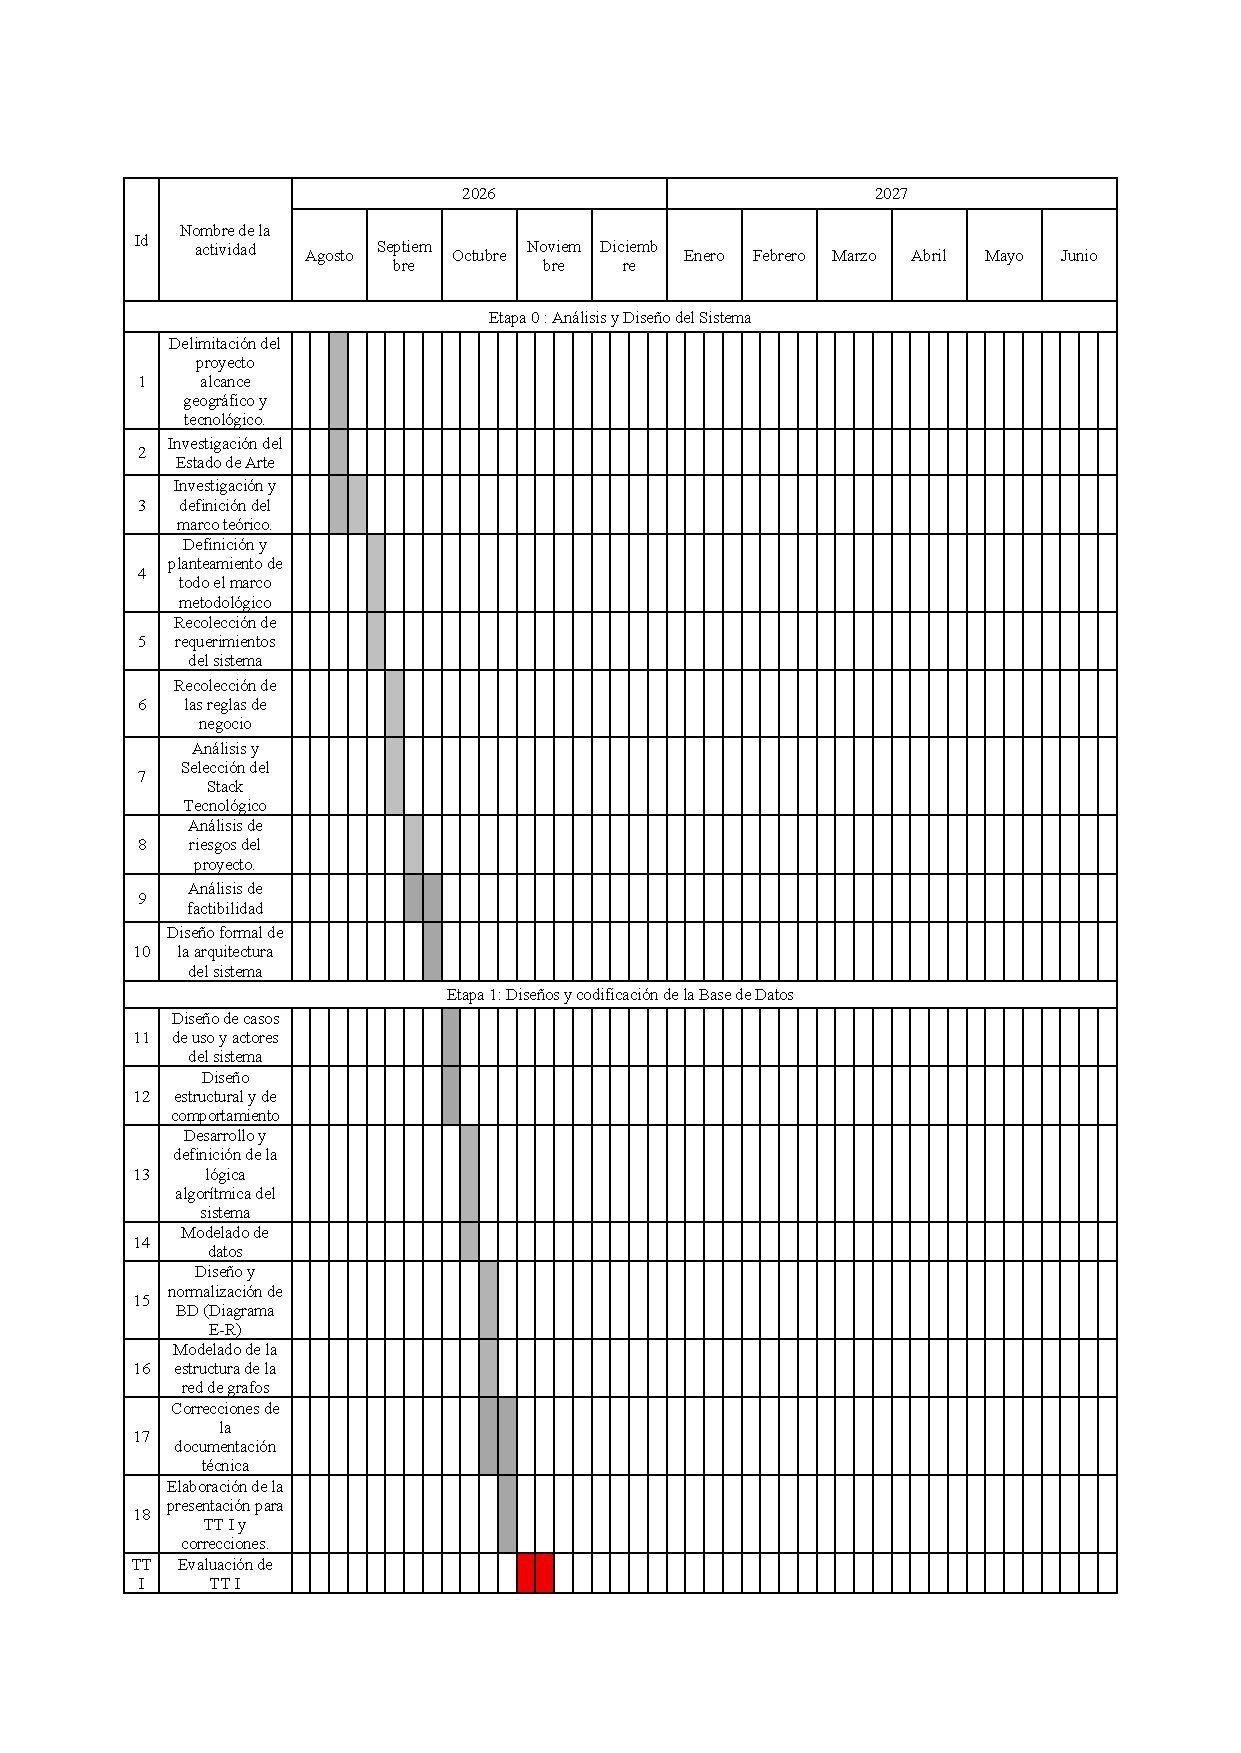
\includegraphics[width=\textwidth, trim={2cm 2cm 2cm 3cm}, clip]{figures/capitulo5_analisis_sistema/5.5_Analisis_de_Factibilidad/Cronograma_2027_TT1.pdf} 
    \caption{Diagrama de Gantt general de actividades del Trabajo Terminal}
    \label{fig:cronograma_actividades}
\end{figure}

\begin{figure}[H]
    \centering
    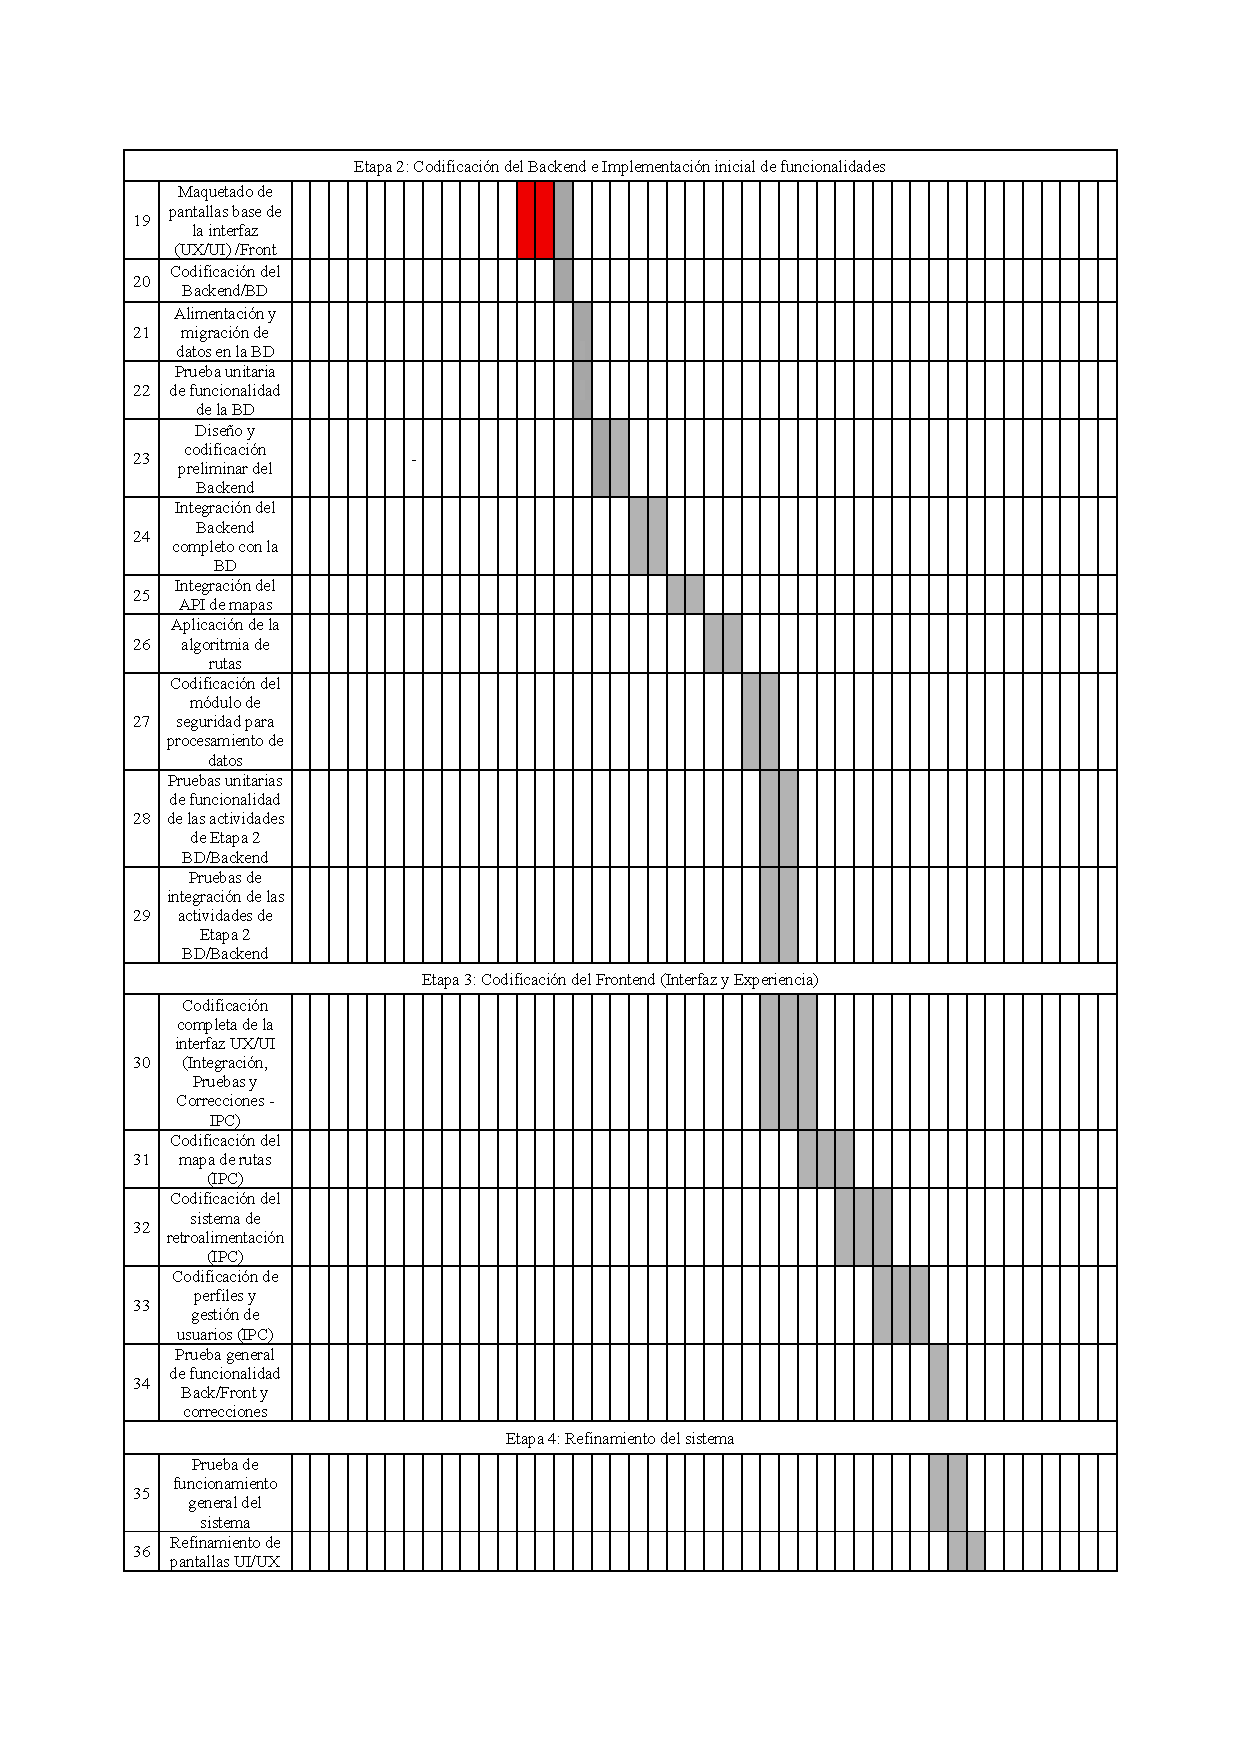
\includegraphics[width=\textwidth, trim={2cm 2cm 2cm 3cm}, clip]{figures/capitulo5_analisis_sistema/5.5_Analisis_de_Factibilidad/Cronograma_2027_TT1-1-2-2.pdf} 
    \caption*{Continuación del diagrama \ref{fig:cronograma_actividades}}
\end{figure}

\begin{figure}[H]
    \centering
    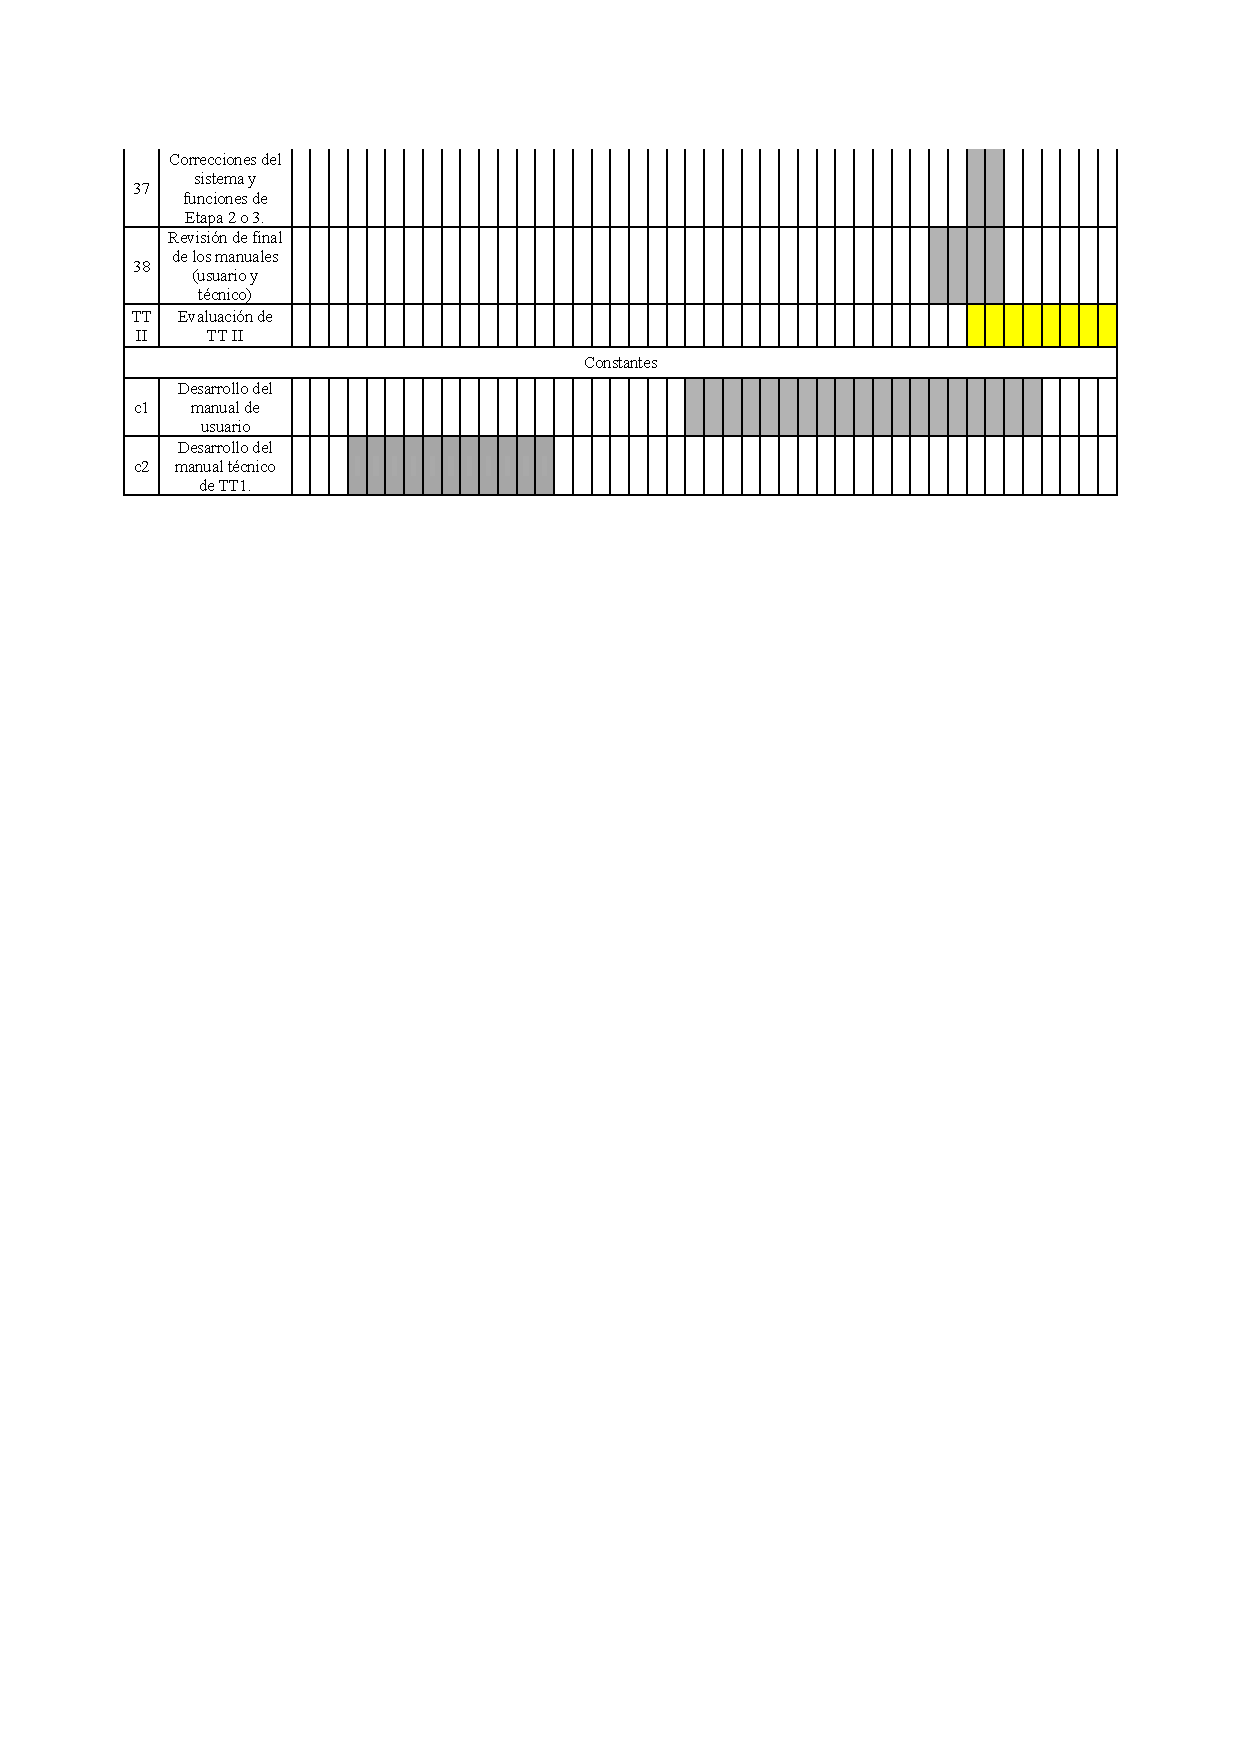
\includegraphics[width=\textwidth, trim={2cm 21cm 2cm 2cm}, clip]{figures/capitulo5_analisis_sistema/5.5_Analisis_de_Factibilidad/Cronograma_2027_TT1-3.pdf} 
    \caption*{Continuación del diagrama \ref{fig:cronograma_actividades}}
\end{figure}

Es necesario realizar la comparación entre el diagrama de Gantt (plazos definidos) contra el tiempo real requerido para el proyecto, de esta forma se observa si realmente el sistema es factible dentro de los intervalos de tiempo establecidos.

En la tabla \ref{tab:resumen_dias} se calcula el tiempo de esfuerzo requerido en base a la cantidad de horas de trabajo que el equipo invierte en el sistema obteniendo la cantidad de días laborales (tomando en cuenta una jornada de tiempo completo; 8 horas) necesarios para el desarrollo dentro del intervalo general de tiempo. 

El plazo de trabajo parte en la tercera semana de Agosto de 2026 y finaliza hasta mediados de Mayo del 2027, considerando que las fechas de presentación de TT I-II se realizan aproximadamente un mes antes de la finalización del periodo escolar. 

\begin{table}[H]
\centering
\renewcommand{\arraystretch}{1.2}
\resizebox{\textwidth}{!}{
\begin{tabular}{l c c c c c c c}
\hline
\textbf{Mes} & \textbf{Días} & \textbf{\makecell{Fin de\\semana}} & \textbf{\makecell{Días no\\laborales}} & \textbf{\makecell{Días\\hábiles}} & \textbf{\makecell{Horas de\\trabajo\\por día\\(promedio)}} & \textbf{\makecell{Horas\\totales}} & \textbf{\makecell{Días\\laborales\\(8 horas\\al día)}} \\ \hline
\textbf{Agosto} & 15 & 4 & 0 & 11 & 4 & 44 & 5.5 \\ 
\textbf{Septiembre} & 30 & 8 & 1 & 21 & 4 & 84 & 10.5 \\ 
\textbf{Octubre} & 31 & 9 & 0 & 22 & 4 & 88 & 11 \\ 
\textbf{Noviembre} & 30 & 9 & 2 & 19 & 4 & 76 & 9.5 \\ 
\textbf{Diciembre} & 30 & 8 & 0 & 22 & 4 & 88 & 11 \\ 
\textbf{Enero} & 31 & 10 & 1 & 20 & 4 & 80 & 10 \\ 
\textbf{Febrero} & 28 & 8 & 1 & 19 & 4 & 76 & 9.5 \\ 
\textbf{Marzo} & 31 & 8 & 3 & 20 & 4 & 80 & 10 \\ 
\textbf{Abril} & 30 & 8 & 5 & 17 & 4 & 68 & 8.5 \\ 
\textbf{Mayo} & 31 & 10 & 2 & 19 & 4 & 76 & 9.5 \\ 
\textbf{Junio} & 7 & 2 & 0 & 5 & 4 & 20 & 2.5 \\ \hline
\textbf{Total} & \textbf{294} & \textbf{84} & \textbf{15} & \textbf{195} & & \textbf{780} & \textbf{97.5} \\ \hline
\end{tabular}
} 
\caption{Resumen de días para el desarrollo del proyecto (Agosto 2026 - Junio 2027) con base a los plazos establecidos en el Diagrama de Gantt \ref{fig:cronograma_actividades}.}
\label{tab:resumen_dias}
\end{table}

Como se aprecia en la tabla \ref{tab:resumen_dias} se cuentan con aproximadamente 98 días laborales para el desarrollo del trabajo terminal considerando una jornada laboral de 8 días, eliminando días festivos, fines de semana y periodos que no entran en el intervalo de tiempo.

%Pendiente por desarrollar el calculo del tiempo real con formulas matematicas de cada actividad para la estimacion real de esfuerzo en tiempo requerido y el contraste con los plazos ya definidos.                                                                                                                                                                                                                            




\subsection{Factibilidad económica}
\label{sec:factibilidad_economica}
A continuación se presenta el análisis de costos asociados al desarrollo del prototipo de aplicación móvil. Los costos de recursos humanos se calculan con base en tarifas de mercado vigentes para cada rol, con el fin de dimensionar el valor económico del trabajo invertido. Por otra parte, los recursos tecnológicos sí representan egresos reales derivados del uso de servicios externos necesarios para el preprocesamiento de datos del sistema. Todos los costos se expresan en pesos mexicanos (MXN) y se acompañan de la fuente y fecha de consulta correspondiente.

\paragraph{Recursos humanos}

Para la realización del proyecto se contempla la participación del equipo de trabajo terminal, compuesto por tres integrantes que colaboran de manera conjunta en todas las etapas del desarrollo, especializándose respectivamente en el diseño y construcción de la base de datos y la lógica algorítmica, el desarrollo de la aplicación móvil, y el análisis y tratamiento de los datos geoespaciales y delictivos. Dado que el proyecto se desarrolla bajo la metodología Scrumban, las funciones de coordinación del equipo son rotativas entre sus integrantes y se ejercen dentro del mismo horario de trabajo individual, por lo que no representan un costo adicional de recursos humanos.

Se considera una dedicación de 2 horas diarias por integrante a lo largo del periodo efectivo de desarrollo del proyecto, comprendido entre el 24 de agosto de 2026 y mediados de mayo de 2027 (aproximadamente 9 meses) conforme al cronograma de actividades. De acuerdo con el Calendario Escolar 2026-2027 del Instituto Politécnico Nacional \cite{ipn_calendario2026}, el cálculo de días hábiles efectivos se obtiene de la siguiente manera:

\begin{align*}
\text{Días hábiles totales (24 ago. 2026 -- 15 may. 2027)} &= 190 \\
(-)\ \text{Días festivos (descanso obligatorio y acuerdo sindical)} &= 12 \\
(-)\ \text{Periodos vacacionales (dic.--ene. y mar.--abr.)} &= 22 \\
\hline
\text{Días hábiles efectivos} &= 156
\end{align*}

\[
156 \text{ días} \times 2 \text{ horas/día} = 312 \text{ horas efectivas por integrante}
\]

La Tabla~\ref{tab:sueldos_mercado} presenta el sueldo mensual promedio en México para cada rol del equipo, obtenido de fuentes de empleo consultado el 6 de octubre del 2026.

\begin{table}[H]
    \centering
    \caption[Sueldo mensual promedio por rol]{Sueldo mensual promedio por rol, según datos de mercado.}
    \vspace{0.2cm}
    \resizebox{\textwidth}{!}{%
    \begin{tabular}{|l|l|c|}
        \hline
        \textbf{Cargo} & \textbf{Fuente} & \textbf{Sueldo mensual promedio} \\ \hline
        Backend Developer & Indeed México \cite{indeed_backend_developer} & \$ 19,210.00 \\ \hline
        Analista de Datos & Indeed México \cite{indeed_analistas_datos} & \$ 15,221.00 \\ \hline
        Desarrollador Móvil & Indeed México \cite{indeed_android_developer} & \$ 17,302.00 \\ \hline
    \end{tabular}%
    }
    \label{tab:sueldos_mercado}
\end{table}

El costo por hora de cada rol se obtiene dividiendo el sueldo mensual promedio entre 160 horas mensuales, correspondientes a una jornada estándar de 8 horas diarias durante 20 días hábiles al mes. Este costo por hora se multiplica por las 312 horas efectivas estimadas por integrante, obteniendo el costo total de recursos humanos mostrado en la Tabla~\ref{tab:recursos_humanos}.

\begin{table}[H]
    \centering
    \caption[Recursos humanos necesarios para realizar el proyecto]{Recursos humanos necesarios para realizar el proyecto. Elaboración propia.}
    \vspace{0.2cm}
    \resizebox{\textwidth}{!}{%
    \begin{tabular}{|l|c|c|c|}
        \hline
        \textbf{Cargo} & \textbf{Horas estimadas} & \textbf{Costo/hora} & \textbf{Costo total} \\ \hline
        Backend Developer & 312 & \$ 120.06 & \$ 37,458.72 \\ \hline
        Analista de Datos & 312 & \$ 95.13 & \$ 29,680.56 \\ \hline
        Desarrollador Móvil & 312 & \$ 108.14 & \$ 33,739.68 \\ \hline
        \multicolumn{3}{|r|}{\textbf{Total}} & \textbf{\$ 100,878.96} \\ \hline
    \end{tabular}%
    }
    \label{tab:recursos_humanos}
\end{table}


\paragraph{Recursos tecnológicos}

Para la realización del proyecto se contempla el uso de los siguientes recursos de hardware, software y servicios en la nube. El equipo de cómputo empleado es propiedad de los integrantes del equipo, por lo que no representa un costo de adquisición adicional para el proyecto. El consumo eléctrico y de internet asociado a su uso durante el desarrollo se contabiliza por separado en la sección de Recursos materiales. Para el desarrollo de la aplicación móvil se emplea el framework Flutter (Dart), mientras que para la gestión de la base de datos y el motor de ruteo geoespacial se utiliza Supabase (PostgreSQL con las extensiones PostGIS y pgRouting), justificado técnicamente en la sección~\ref{sec:factibilidad_técnica}.

El plan gratuito de Supabase ofrece 500 MB de base de datos, 500 MB de almacenamiento de archivos, 5 GB de transferencia de datos mensual y solicitudes de API ilimitadas \cite{supabase_pricing}. El polígono de estudio delimitado en la Figura~\ref{fig:mapa_zona_estudio} abarca una superficie de 26.31 km\textsuperscript{2} y su red vial comprende aproximadamente 11{,}700 segmentos de calle. Considerando un peso promedio de 1 a 3 KB por segmento, el volumen estimado de la base de datos se ubica entre 12 y 35 MB, muy por debajo del límite mencionado, por lo que se opta por el plan gratuito.

Para el preprocesamiento de la información se emplea la Street View Static API de Google Maps Platform, mediante la cual se obtendrán tres imágenes por cada segmento de calle, es decir, aproximadamente 35{,}100 solicitudes. Esta API ofrece una cuota gratuita de 10{,}000 solicitudes mensuales y cobra \$7.00 USD por cada 1{,}000 solicitudes adicionales \cite{google_maps_pricing}, por lo que se generarían 25{,}100 solicitudes facturables, equivalentes a \$175.70 USD (\$3,156.80 MXN). Posteriormente, las imágenes se analizan con el modelo Qwen3.7-Flash \cite{qwen_pricing}, cuyo costo para solicitudes de hasta 32{,}000 tokens es de \$0.03 USD por millón de tokens de entrada y \$0.13 USD por millón de tokens de salida. Considerando un consumo aproximado de 2{,}000 tokens de entrada y 500 de salida por imagen, el análisis de las 35{,}100 imágenes requiere 70.2 millones de tokens de entrada y 17.55 millones de salida, con un costo total de \$4.39 USD (\$78.83 MXN). Durante la operación de la aplicación se utiliza el SDK de Maps para dispositivos móviles, cuyo uso es ilimitado y sin costo, y Places API (New), cuyas SKU de Autocomplete y Place Details Essentials incluyen 10{,}000 solicitudes gratuitas mensuales cada una \cite{google_maps_pricing}. Los montos expresados en dólares estadounidenses se convirtieron a pesos mexicanos con el tipo de cambio FIX publicado por el Banco de México el 6 de octubre de 2026, equivalente a \$17.9670 MXN por dólar \cite{banxico_fix}.

Adicionalmente, el equipo utiliza dos servicios por suscripción mensual durante el desarrollo del proyecto: Overleaf, para la redacción del documento en LATEX, y Udemy, para la capacitación técnica de los integrantes. Considerando una duración de nueve meses, el costo de estos servicios se desglosa en la Tabla~\ref{tab:servicios_adicionales}.

El proyecto contempla como entregable un prototipo funcional de la aplicación móvil, cuya conclusión no depende de su publicación en una tienda de aplicaciones. No obstante, de presentarse la oportunidad, el prototipo podrá publicarse en Google Play Store, lo que requiere un pago único de registro de desarrollador de \$25.00 USD (\$449.18 MXN) \cite{google_play_console}. Al tratarse de un gasto opcional, no se incluye en el total del presupuesto.

\begin{table}[H]
    \centering
    \caption[Recursos tecnológicos necesarios para realizar el proyecto]{Recursos tecnológicos necesarios para realizar el proyecto. Elaboración propia.}
    \vspace{0.2cm}
    \resizebox{\textwidth}{!}{%
    \begin{tabular}{|l|l|c|}
        \hline
        \textbf{Cantidad} & \textbf{Descripción} & \textbf{Costo} \\ \hline
        \multicolumn{3}{|l|}{\textit{Hardware}} \\ \hline
        3 & Equipo de cómputo propio del equipo & \$ 0.00 \\ \hline
        \multicolumn{3}{|l|}{\textit{Software y servicios en la nube}} \\ \hline
        1 & Flutter / Dart (código abierto) & \$ 0.00 \\ \hline
        1 & Supabase -- plan gratuito (PostgreSQL, PostGIS, pgRouting) & \$ 0.00 \\ \hline
        1 & Git / GitHub (plan gratuito) & \$ 0.00 \\ \hline
        1 & Google Meet (plan gratuito) & \$ 0.00 \\ \hline
        1 & Notion (plan estudiante, gratuito) & \$ 0.00 \\ \hline
        \multicolumn{3}{|l|}{\textit{APIs de preprocesamiento (35{,}100 imágenes: 11{,}700 segmentos $\times$ 3)}} \\ \hline
        35{,}100 & Google Street View Static API (10{,}000 gratuitas; 25{,}100 a \$7.00 USD/1{,}000) & \$ 3,156.80 \\ \hline
        35{,}100 & Qwen3.7-Flash, análisis de imágenes (70.2 M tokens de entrada y 17.55 M de salida) & \$ 78.83 \\ \hline
        \multicolumn{3}{|l|}{\textit{APIs de operación de la aplicación}} \\ \hline
        1 & Maps SDK para móvil (uso ilimitado sin costo) & \$ 0.00 \\ \hline
        1 & Places API (New), dentro de la cuota gratuita & \$ 0.00 \\ \hline
        \multicolumn{3}{|l|}{\textit{Opcional (no incluido en el total)}} \\ \hline
        1 & Registro de desarrollador Google Play (pago único) & \$ 449.18 \\ \hline
        \multicolumn{2}{|r|}{\textbf{Total}} & \textbf{\$ 3,235.63} \\ \hline
    \end{tabular}%
    }
    \label{tab:recursos_tecnologicos}
\end{table}

\begin{table}[H]
    \centering
    \caption[Servicios adicionales por suscripción mensual]{Servicios adicionales por suscripción mensual. Elaboración propia.}
    \vspace{0.2cm}
    \resizebox{\textwidth}{!}{%
    \begin{tabular}{|c|l|c|c|}
        \hline
        \textbf{Meses} & \textbf{Descripción} & \textbf{Costo mensual} & \textbf{Costo total} \\ \hline
        9 & Overleaf (suscripción mensual) & \$ 99.00 & \$ 891.00 \\ \hline
        9 & Udemy (suscripción mensual) & \$ 209.00 & \$ 1,881.00 \\ \hline
        \multicolumn{3}{|r|}{\textbf{Total}} & \textbf{\$ 2,772.00} \\ \hline
    \end{tabular}%
    }
    \label{tab:servicios_adicionales}
\end{table}

\paragraph{Recursos materiales}

Para la realización del proyecto se contemplan los siguientes recursos materiales asociados a la operación básica del equipo de trabajo. El costo de la energía eléctrica se estima a partir del consumo de los equipos de cómputo durante las horas efectivas de trabajo. Considerando las 312 horas efectivas por integrante calculadas en la sección de recursos humanos, y una potencia aproximada de 65 W por equipo, el consumo se obtiene de la siguiente manera:

\begin{align*}
\text{Horas de uso} &= 312 \text{ h} \times 3 \text{ integrantes} = 936 \text{ h} \\
\text{Consumo} &= 936 \text{ h} \times 0.065 \text{ kW} = 60.84 \text{ kWh} \approx 61 \text{ kWh}
\end{align*}

Dicho consumo se valora con la cuota del consumo excedente de la Tarifa 1 de la Comisión Federal de Electricidad para octubre de 2026, equivalente a \$4.054 por kilowatt-hora \cite{cfe_tarifa1}, considerada como valor conservador. Respecto al servicio de internet, cada integrante cuenta con un paquete residencial de 100 Mbps con costo mensual de \$390.00 \cite{totalplay_paquetes}, el cual se contabiliza durante los 9 meses de desarrollo del proyecto.

\begin{table}[H]
    \centering
    \caption[Recursos materiales necesarios para realizar el proyecto]{Recursos materiales necesarios para realizar el proyecto. Elaboración propia.}
    \vspace{0.2cm}
    \resizebox{\textwidth}{!}{%
    \begin{tabular}{|l|l|c|c|}
        \hline
        \textbf{Cantidad} & \textbf{Descripción} & \textbf{Costo} & \textbf{Total} \\ \hline
        61 & Energía eléctrica, Tarifa 1 CFE (kWh) & \$ 4.054 & \$ 247.29 \\ \hline
        27 & Internet residencial 100 Mbps (3 integrantes $\times$ 9 meses) & \$ 390.00 & \$ 10,530.00 \\ \hline
        \multicolumn{3}{|r|}{\textbf{Total}} & \textbf{\$ 10,777.29} \\ \hline
    \end{tabular}%
    }
    \label{tab:recursos_materiales}
\end{table}


\paragraph{Flujo de pago}

El costo total estimado del proyecto se resume en la Tabla~\ref{tab:flujo_pago} y asciende a \$129,430.27 MXN, que resulta de sumar los recursos humanos, tecnológicos y materiales (\$117,663.88 MXN) y un 10\% de imprevistos calculado sobre dicho subtotal (\$11,766.39 MXN). No se considera el pago opcional de registro en Google Play Store. De este monto, \$100,878.96 corresponden al valor de mercado del trabajo del equipo, el cual, al ser realizado directamente por los integrantes del trabajo terminal sin una relación de contratación formal, no representa un desembolso. De igual forma, los recursos materiales (energía eléctrica e internet) corresponden a servicios que los integrantes ya tienen contratados, por lo que se contabilizan para dimensionar el costo real del proyecto sin implicar un gasto adicional. En consecuencia, el egreso efectivo se limita a los recursos tecnológicos, por un monto de \$6,007.63 MXN, equivalente a aproximadamente \$2,002.54 MXN por integrante a lo largo de los nueve meses de desarrollo (\$222.50 MXN mensuales).

Con base en lo anterior, el proyecto se considera económicamente viable: el gasto efectivo es reducido y proviene principalmente de servicios de preprocesamiento de uso único y de suscripciones mensuales, mientras que el resto de los costos corresponde a trabajo y recursos que el equipo ya posee o tiene contratados.

\begin{table}[H]
    \centering
    \caption[Resumen de costos totales del proyecto]{Resumen de costos totales del proyecto. Elaboración propia.}
    \vspace{0.2cm}
    \begin{tabular}{|l|c|}
        \hline
        \textbf{Recursos} & \textbf{Costo} \\ \hline
        Recursos Humanos & \$ 100,878.96 \\ \hline
        Recursos Tecnológicos & \$ 6,007.63 \\ \hline
        Recursos Materiales & \$ 10,777.29 \\ \hline
        Subtotal & \$ 117,663.88 \\ \hline
        Imprevistos (10\%) & \$ 11,766.39 \\ \hline
        \textbf{Total} & \textbf{\$ 129,430.27} \\ \hline
    \end{tabular}
    \label{tab:flujo_pago}
\end{table}

\subsection{Factibilidad legal}
\label{sec:factibilidad_legal}
En este apartado se analiza la factibilidad legal del proyecto, donde se verifica el cumplimiento de los requisitos jurídicos y si esta dentro de las leyes, normas y reglamentos vigentes del marco jurídico sin llegar a infringir leyes, derechos de autor o licencias de terceros.  



\subsection{Factibilidad de recursos}
\label{sec:factibilidad_recursos}
\input{documents/capitulo5_analisis_sistema/5.5_Analisis_de_Factibilidad/5.5.5_Factibilidad_recursos/seccion5_5_5}






% =========================================================
% CAPÍTULO 6: DISEÑO DEL SISTEMA
% =========================================================
\chapter{Diseño del sistema}
\label{cap:diseno_sistema}
% =========================================================
% ARQUITECTURA DEL SISTEMA Y TECNOLOGÍAS
% =========================================================
\section{Arquitectura del sistema}
\subsection{Diagrama de contexto}
\subsection{Diagrama de contenedores}
\subsection{Diagrama de componentes}

% =========================================================
% CASOS DE USO
% =========================================================
\section{Casos de uso}
\subsection{Diagrama de casos de uso}
\subsection{Actores}
\subsubsection{Especificación de Casos de Uso}

% =========================================================
% MODELADO ESTRUCTURAL Y DE COMPORTAMIENTO
% =========================================================
\section{Diseño estructural y de comportamiento}
\subsection{Diagramas de secuencia}
\subsection{Diagramas de código}
\subsection{Diagrama de clases}
\subsection{Diagramas de actividades}

% =========================================================
% DISEÑO DE DATOS Y MODELO GEOESPACIAL
% =========================================================
\section{Diseño de base de datos}
\subsection{Modelo entidad-relación}
\subsection{Estructura y persistencia de la red de grafos}


% =========================================================
% LÓGICA ALGORÍTMICA
% =========================================================
\section{Lógica algorítmica y procesamiento geoespacial}
\subsection{Diseño del algoritmo de asignación de costos}
\subsection{Diseño del motor de ruteo (\texorpdfstring{$A^*$}{A*})}

% =========================================================
% INTERFACES DE USUARIO
% =========================================================
\section{Diseño de interfaces de usuario (UI/UX)}




% *************************************************
% SECCIONES PARA TT 2

% =========================================================
% CAPÍTULO 7: DESARROLLO E IMPLEMENTACIÓN 
% =========================================================
\chapter{Desarrollo e Implementación}
\label{cap:desarrollo_implementacion}
% =========================================================
% CAPÍTULO 7: DESARROLLO E IMPLEMENTACIÓN
% Cada sección vive en su carpeta 7.X_<nombre>/ con su
% seccion7_X.tex (contenido) y seccion7_X.bib (referencias).
% =========================================================

% =========================================================
% 7.1 PREPROCESAMIENTO DE DATOS Y MODELO DE RIESGO
% =========================================================
\section{Preprocesamiento de datos y modelo de riesgo}
\label{sec:impl_modelo_riesgo}
% =========================================================
% 7.1 PREPROCESAMIENTO DE DATOS Y MODELO DE RIESGO
% El \section{} de esta sección está en el chapter.tex del capítulo;
% sus referencias van en seccion7_1.bib (misma carpeta).
% =========================================================

% Contenido pendiente.


% =========================================================
% 7.2 BASE DE DATOS Y RED DE GRAFOS
% =========================================================
\section{Base de datos y red de grafos}
\label{sec:impl_base_datos}
% =========================================================
% 7.2 BASE DE DATOS Y RED DE GRAFOS
% El \section{} de esta sección está en el chapter.tex del capítulo;
% sus referencias van en seccion7_2.bib (misma carpeta).
% =========================================================

% Contenido pendiente.


% =========================================================
% 7.3 MOTOR DE RUTEO
% =========================================================
\section{Motor de ruteo}
\label{sec:impl_motor_ruteo}
% =========================================================
% 7.3 MOTOR DE RUTEO
% El \section{} de esta sección está en el chapter.tex del capítulo;
% sus referencias van en seccion7_3.bib (misma carpeta).
% =========================================================

% Contenido pendiente.


% =========================================================
% 7.4 APLICACIÓN MÓVIL
% =========================================================
\section{Aplicación móvil}
\label{sec:impl_aplicacion_movil}
% =========================================================
% 7.4 APLICACIÓN MÓVIL
% El \section{} de esta sección está en el chapter.tex del capítulo;
% sus referencias van en seccion7_4.bib (misma carpeta).
% =========================================================

% Contenido pendiente.




% =========================================================
% CAPÍTULO 8: PRUEBAS
% =========================================================
\chapter{Pruebas}
\label{cap:pruebas}
% =========================================================
% CAPÍTULO 8: PRUEBAS
% Cada sección vive en su carpeta 8.X_<nombre>/ con su
% seccion8_X.tex (contenido) y seccion8_X.bib (referencias).
% =========================================================

% =========================================================
% 8.1 VALIDACIÓN DEL MODELO DE RIESGO
% =========================================================
\section{Validación del modelo de riesgo}
\label{sec:validacion_modelo_riesgo}
% =========================================================
% 8.1 VALIDACIÓN DEL MODELO DE RIESGO
% El \section{} de esta sección está en el chapter.tex del capítulo;
% sus referencias van en seccion8_1.bib (misma carpeta).
% =========================================================

% Contenido pendiente.


% =========================================================
% 8.2 PRUEBAS UNITARIAS
% =========================================================
\section{Pruebas unitarias}
\label{sec:pruebas_unitarias}
% =========================================================
% 8.2 PRUEBAS UNITARIAS
% El \section{} de esta sección está en el chapter.tex del capítulo;
% sus referencias van en seccion8_2.bib (misma carpeta).
% =========================================================

% Contenido pendiente.


% =========================================================
% 8.3 PRUEBAS FUNCIONALES
% =========================================================
\section{Pruebas funcionales}
\label{sec:pruebas_funcionales}
% =========================================================
% 8.3 PRUEBAS FUNCIONALES
% El \section{} de esta sección está en el chapter.tex del capítulo;
% sus referencias van en seccion8_3.bib (misma carpeta).
% =========================================================

% Contenido pendiente.


% =========================================================
% 8.4 COMPARACIÓN DE LA EXPOSICIÓN AL RIESGO
% =========================================================
\section{Comparación de la exposición al riesgo}
\label{sec:comparacion_exposicion}
% =========================================================
% 8.4 COMPARACIÓN DE LA EXPOSICIÓN AL RIESGO
% El \section{} de esta sección está en el chapter.tex del capítulo;
% sus referencias van en seccion8_4.bib (misma carpeta).
% =========================================================

% Contenido pendiente.



% *************************************************

% =========================================================
% CAPÍTULO 9: CONCLUSIONES Y TRABAJO FUTURO
% =========================================================
\chapter{Conclusiones y trabajo futuro}
\label{cap:conclusiones}
% =========================================================
% CAPÍTULO 9: CONCLUSIONES Y TRABAJO FUTURO
% Cada sección vive en su carpeta 9.X_<nombre>/ con su
% seccion9_X.tex (contenido) y seccion9_X.bib (referencias).
% =========================================================

% =========================================================
% 9.1 CONCLUSIONES
% =========================================================
\section{Conclusiones}
\label{sec:conclusiones}
% =========================================================
% 9.1 CONCLUSIONES
% El \section{} de esta sección está en el chapter.tex del capítulo;
% sus referencias van en seccion9_1.bib (misma carpeta).
% =========================================================

% Contenido pendiente.


% =========================================================
% 9.2 TRABAJO FUTURO
% =========================================================
\section{Trabajo futuro}
\label{sec:trabajo_futuro}
% =========================================================
% 9.2 TRABAJO FUTURO
% El \section{} de esta sección está en el chapter.tex del capítulo;
% sus referencias van en seccion9_2.bib (misma carpeta).
% =========================================================

% Contenido pendiente.



% =========================================================
% REFERENCIAS / BIBLIOGRAFÍA
% =========================================================
\renewcommand{\bibname}{Referencias}
\addcontentsline{toc}{chapter}{Referencias}

\bibliographystyle{IEEEtran}
\bibliography{
% Capítulo 1
documents/capitulo1_antecedentes/chapter,
% Capítulo 2
documents/capitulo2_estado_arte/chapter,
% Capítulo 3
documents/capitulo3_marco_teorico/3.1_criminologia_ambiental/seccion3_1,
documents/capitulo3_marco_teorico/3.2_contexto_geografico/seccion3_2,
documents/capitulo3_marco_teorico/3.5_teoria_de_grafos/seccion3_5,
% Capítulo 4
documents/capitulo4_marco_metodologico/chapter,
% Capítulo 5
documents/capitulo5_analisis_sistema/5.1_Requerimientos/seccion5_1,
documents/capitulo5_analisis_sistema/5.2_Reglas_negocio/seccion5_2,
documents/capitulo5_analisis_sistema/5.3_Analisis_de_herramientas_a_utilizar/seccion5_3,
documents/capitulo5_analisis_sistema/5.4_Analisis_de_riesgos/seccion5_4,
documents/capitulo5_analisis_sistema/5.5_Analisis_de_Factibilidad/seccion5_5
}

\end{document}